\documentclass[	pdftex, 
								a4paper,
								11pt, DIV11, BCOR5mm,
								parskip,
								%openany,
								]{scrreprt}
\usepackage[utf8]{inputenc}
\usepackage[T1]{fontenc}

\usepackage[colorlinks=true,linkcolor=blue,citecolor=blue]{hyperref}
\usepackage{comment}
\usepackage[english]{babel}
\usepackage[nonumberlist,toc,acronym]{glossaries}

\usepackage{fancyhdr}
\usepackage[section]{placeins}
\usepackage{graphicx}
\usepackage{listings}
\usepackage[german]{babelbib}
\usepackage{array}
\usepackage{wrapfig}
\usepackage{varwidth}
\usepackage{float}
\usepackage{dirtree}
\usepackage{epstopdf}
\usepackage{textpos}
\usepackage{changepage}
\usepackage{theorem}
\usepackage{caption}
\usepackage{framed}
\usepackage{booktabs}
\usepackage{tikz}
\usetikzlibrary{decorations.markings,arrows,positioning,trees,calc,fit,shapes}
\usepackage[noend]{algorithmic}
\usepackage{amsmath}
\usepackage{algorithm}
\usepackage{environ}
\usepackage{ulem}

%Kopfzeile hinzufuegen
\renewcommand{\sectionmark}[1]{\markboth{#1}{}} % set the \leftmark

\fancypagestyle{plain}{
    
    \fancyhead[R]{\leftmark}
    
    \renewcommand{\headrulewidth}{1pt}
    %\fancyfoot[R]{\thepage}
}

\pagestyle{fancy}

%Literaturverzeichnis hinzufuegen
\bibliographystyle{babplain}

% Glossar hinzufuegen
\makeglossaries
\newacronym{usda} {USDA}{US Department of Agriculture}
\newacronym{fdc}{FDC}{FoodData Central}
\newacronym{rest}{REST}{Representational state transfer}
\newacronym{dge}{DGE}{Deutsche Gesellschaft für Ernährung}
\newacronym{pal}{PAL-Value}{physical activity level-Value}
\newacronym{json}{JSON}{JavaScript Object Notation}
\newacronym{iri}{IRI}{International Resource Identifier}
\newacronym{http}{HTTP}{HyperText Transfer Protocol}
\newacronym{xml}{XML}{Extensible Markup Language}
\newacronym{cdno}{CDNO}{Compositional Dietary Nutrition Ontology}
\newacronym{obo}{OBO}{Open Biological and Biomedical Ontology}
\newacronym{sparql}{SPARQL}{SPARQL Protocol And RDF Query Language}
\newacronym{sql}{SQL}{Structured Query Language}
\newacronym{uri}{URI}{Uniform Resource Identifier}
\newacronym{gi}{GI}{Glykämischer Index}
\newacronym{bmi}{BMI}{Body-Mass-Index}



\begin{document}
\setcounter{page}{-2}
\pagestyle{empty}
\pagenumbering{none}
\newcommand{\firstreviewer}{Prof. Michael Beetz PhD}
\newcommand{\secondreviewer}{Prof. Dr. Nico Hochgeschwender}
\newcommand{\supervisor}{Dr. Michaela Kümpel, Vanessa Hassouna}
\newcommand{\thesistype}{Master Thesis}
\newcommand{\myauthor}{Naser Azizi, Sorin Arion}
\newcommand{\mymaintitle}{A Knowledge Base with which You Can Parameterize Robot Plans for Multiple Mixing Actions}
\newcommand{\mytitle}{\centering {\Huge \mymaintitle}\\[.3in] 
    {\Large \mysubtitle}}
\newcommand{\pdftitle}{\mymaintitle - \mysubtitle}
\newcommand{\formattedfronttitle}{{\mytitle}}
\newcommand{\formattedinnertitle}{{\mytitle}}

\begin{titlepage}
	\vspace*{-2.2cm}
	\begin{adjustwidth}{-0cm}{-2.3cm}
	\thispagestyle{empty}
        \begin{figure}
            \begin{minipage}{.4\linewidth}
	\begin{flushleft}
		
\includegraphics[height=1.5cm]{Graphics/unilogo-transp.pdf}
	\end{flushleft}
    \end{minipage}
    \hspace{.2\linewidth}
            \begin{minipage}{.4\linewidth}
	\begin{flushright}
		
\includegraphics[height=3.0cm]{Graphics/logo-ai-small.pdf}
	\end{flushright}
    \end{minipage}
\end{figure}
	  \vfill
	  %\scalebox{0.95}{
    	  %\begin{minipage}{1.2\textwidth}
    	  %{
    		%\formattedfronttitle 
    	  %}
    	  %\end{minipage}
	  %}
	\begin{center}
	  {\huge \mymaintitle}\\
	  
	  \vfill
	  {\Large \thesistype}\\[2.5ex]
	  {\Large\em \myauthor}
	  \vfill
	{  
      \renewcommand\arraystretch{1.5}
      \begin{tabular}{l@{\hspace{2em}}r@{\hspace{1ex}}p{7cm}}
     Pr\"ufer der \thesistype: & 1. & \firstreviewer\\
                                 & 2. & \secondreviewer\\
	Supervisor		    &   & \supervisor\\
   \end{tabular}
  }
	\end{center}
	\end{adjustwidth}
\end{titlepage}
	\pagenumbering{arabic}
	\setcounter{page}{1}
	\pagestyle{plain}
	%\addcontentsline{toc}{chapter}{Eidesstaatliche Erkl\"arung}
	\chapter*{Eidesstattliche Erkl\"arung}
	
	Hiermit erkl\"aren wir, dass die vorliegende Arbeit selbstst\"andig angefertigt,
	nicht anderweitig zu Pr\"ufungszwecken vorgelegt und keine anderen als die
	angegebenen Hilfsmittel verwendet habe. S\"amtliche wissentlich verwendete
	Textausschnitte, Zitate oder Inhalte anderer Verfasser wurden ausdr\"ucklich als
	solche gekennzeichnet.
	
	Bremen, den \makeatletter\@date\makeatother
	
	\vspace*{1em}
	\rule{15em}{0.16667pt}\\
	\author{Naser Azizi, Sorin Arion}
	\makeatletter\@author\makeatother
	
	
	\normalem
	%Abstrakt
	%\addcontentsline{toc}{chapter}{Abstract}


\chapter*{Motivation}

Although industrial robots have been considered standard for many years, 
the widespread adoption of AI-based autonomous household robots is still far from being anticipated in every household. 
Obstacles such as unfamiliar surroundings and a limited knowledge base can significantly hinder the ability of an autonomous robot to effectively respond in a given situation.
 Hence, the robot must precisely plan for every minor detail, even those that might appear trivial to us humans.

To achieve the defined objectives, a proficient and comprehensive robotic system including control, perception, navigation, and knowledge is necessary.
An illustrative goal could be cooking. To execute this task, the robot must possess various capabilities, including placing items, grasping objects, 
pouring liquids, cutting ingredients, and mixing components. These tasks seem trivial to us humans, but for robots, they require extensive implementation and information.

In this thesis, we aim to introduce an approach detailing how a robotic system can execute mixing actions effectively. 
The challenges arise from the diverse methods of mixing, which further vary based on the specific ingredients being combined. 
Additionally, the consideration of compatible mixing tools and mixing containers is crucial, as not every tool can be utilized with every container.

Through the incorporation of a knowledge graph containing rules related to various actions, 
we aim to empower the robotic system to make informed decisions on the appropriate motions to employ. 
This decision-making process will take into account the specific task at hand and the involved ingredients. 
By incorporating this knowledge graph, we aim to advance towards autonomous robots capable of engaging in cooking activities.

\tableofcontents
\chapter{Introduction}
This master's thesis addresses the issue of mixing and its variations in the context of cooking as high-level tasks, taking into account contextual knowledge, to derive statements about which mixing movements a robotic agent should perform using a knowledge base.

Before presenting the structure of the master's thesis, we address five essential aspects to provide readers with a better overview. The problem at hand involves various tasks in the world of cooking and baking. While humans learn over their lifetime how to prepare recipes and intuitively execute the necessary actions, a robot must have these required actions readily available. A robot's tasks in cooking can be diverse, such as cutting, pouring, or mixing. This thesis focuses on the task of mixing and examines the issue of different mixing actions and the context in which they are performed. 

The importance of considering various movements to achieve desired results in mixing is emphasized, as a single movement cannot suffice for different outcomes. Different movements must be taken into account to achieve the desired results of a mixing action. The difficulty arises from the lack of a systematic approach to determine which mixing movement should be performed under specific circumstances. A systematic approach, primarily utilizing video material, is necessary to identify the relationships between the actions performed by humans, the ingredients used, and the associated movements. The biggest challenge lies in deciding how to model this knowledge in a symbolic knowledge base so that the relevant knowledge is usable for the robot.

To solve this problem, the analysis of videos is employed to determine how general principles can be inferred from individual cases, especially regarding human actions during the mixing of ingredients. Both the nature of the ingredients and the movements executed are considered. The identified relationships are modeled in a knowledge base, allowing a robotic agent to derive possible movements with the necessary parameters for execution. The knowledge base is symbolically modeled, enabling theoretical support for execution by many robotic agents.

The knowledge base should be used by     to execute various motions accordingly, taking into account defined parameters that adapt to the geometric characteristics of the containers and tools. 
This involves extracting geometric information and defining specific action ranges for the motions.

This work contributes to research by enabling robotic agents to query the required knowledge for mixing actions. The implementation of our knowledge base aims at developing robots capable of performing non-trivial tasks autonomously in household settings without a predefined environment.


Our work is divided into multiple chapters that will cover every aspect of our research and practical work.
First, we intend to analyze existing research, particularly examining studies that delve into diverse mixing motions and exploring related systems that contain a queryable knowledge graph(\ref{chap:Related_work}).

In the following section, we will introduce the reader with the frameworks employed to accomplish our objectives (\ref{chap:libraries}).	
Subsequently, we will present our approach to data acquisition and data representation (\ref{chap:Data_acquisition}, \ref{chap:Data_representation}).
In this chapters, we aim to explain the mixing tasks under consideration and articulate our methodology for representing this data to enable effective querying.
In the subsequent section, we will illustrate the implementation of our rules, with the ultimate aim of determining the appropriate motion to be employed.

To validate our concept, we have opted to simulate various scenarios and assess their outcomes, demonstrating the efficacy of our implemented system (\ref{chap:Execution on the robot}).

Before we will delve into the discussion of our results and draw conclusions to wrap up our work, we want to present a newly implemented web framework for graph visualization (\ref{chap:OWLViz}).

The following graphic is intended to provide an overview and will be referenced in each chapter to indicate which part of the work the chapter is addressing.
\begin{figure}[H]
    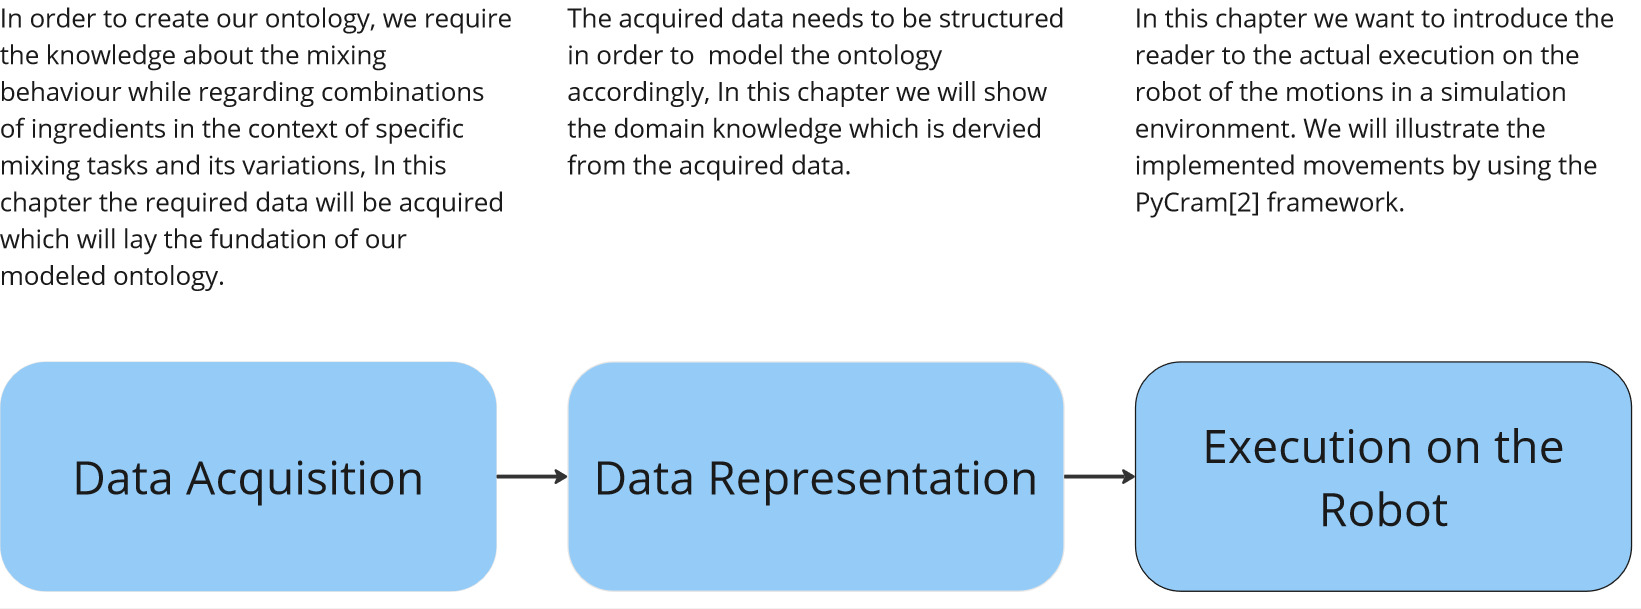
\includegraphics[scale=0.25]{Graphics/structure_overview.jpg}
    \caption{Structure overview}
\end{figure}	

\chapter*{Related Work}
\begin{itemize}
    \item \url{https://ieeexplore.ieee.org/stamp/stamp.jsp?tp=&arnumber=1641754}
    \item \url{https://ieeexplore.ieee.org/stamp/stamp.jsp?tp=&arnumber=8954776}
    \item \url{https://robomechjournal.springeropen.com/articles/10.1186/s40648-021-00204-6}
    \item \url{https://www.researchgate.net/profile/Daniela_Rus/publication/265243176_BakeBot_Baking_Cookies_with_the_PR2/links/56d043ad08aeb52500cd34a0.pdf}
    \item \url{https://ieeexplore.ieee.org/stamp/stamp.jsp?tp=&arnumber=9083695}
    \item \url{https://ieeexplore.ieee.org/stamp/stamp.jsp?tp=&arnumber=7301404}
    \item \url{https://ieeexplore.ieee.org/abstract/document/8460964}
    \item \url{https://ieeexplore.ieee.org/stamp/stamp.jsp?tp=&arnumber=9096241}
    \item \url{https://ieeexplore.ieee.org/stamp/stamp.jsp?tp=&arnumber=10004056}
    \item \url{https://robbreport.com/gear/electronics/moley-robotics-robot-kitchen-uk-for-sale-1234590791/}
    \item \url{https://ieeexplore.ieee.org/stamp/stamp.jsp?tp=&arnumber=8310925}
    \item \url{https://ieeexplore.ieee.org/stamp/stamp.jsp?tp=&arnumber=7523919}
    \item \url{https://ieeexplore.ieee.org/stamp/stamp.jsp?tp=&arnumber=7523919}
\end{itemize}

There are multiple approaches for mixing tasks in the kitchen domain. From high level symbolic to low level motions and 
learning approaches, these different approaches, tries to tackle the challenge of solving mixing in the kitchen environment.

FoodCutting aims to equip robotic agents with necessary information about how to 
execute  cutting tasks in unknown environments for the household domain. From high level plans FoodCutting breaks down 
the cutting task, part of some robot plan, into executable motions regarding cutting fruits and vegetables. These motions are parameterized 
by some technique and repetitions to achieve the agents objective. 
FoodCutting does not require fully available knowledge
about the agents environment, instead the robot should be capable of recognizing certain objects for cutting 
operations. 

BakeBot realised on the PR2 robotics platform attempts to achieve baking cookies. An implementation of locating relevant things for MixingTasks
like a bowl and ingredients has been realised for semi-structured environments. An algorithm to perform mixing motions has been implemented as well, to mix 
ingredients with different characteristics into an uniform dough. These motions are limited to a simple circular and linear mixing motion.
The authors follow an bottom-up approach which is inherently motion driven rather than a
symbolic one which attempts to break down high level tasks into executable low level motions. 

FluidLab is a simulation environment for different kinds of manipulation tasks regarding liquids. Its underlying engine uses differentiable physics 
enabling reinforcement learning and optimization techniques in manipulation to utilize the engine, to achieve several tasks 
including liquids and solids, like mixing tasks. 

Our mixing approach will be most similar to the FoodCutting approach, in which we model symbolic knowledge about how to perform
mixing tasks, which technique should be used and infering parameters for the execution of the underlying motion.



    \chapter{Introduction to Hardware and Software components}
    This chapter serves as an introduction to the frameworks, software, and libraries we use. The work we present can be simplified explained as a knowledge base containing parameters that a robot can use to perform specific actions.

    Firstly, we would like to introduce the robotic component, which acts as the interface between the knowledge base we have created and the robot, followed by an introduction to Ontologies and Knowledgebases.
    \section{Robotic section: ROS and PyCRAM}
    
    The main framework we use is \textit{PyCRAM} \cite{pycram}, which serves as an interface for various software components such as knowledge, perception, or manipulation. 
	This framework utilizes another framework, \textit{ROS} (Robotic Operating System) \cite{ros}, to communicate with the different robot components. These two frameworks are now introduced in the following.    
    \subsection{ROS}
	\label{sec:ROS}
    \begin{wrapfigure}{r}{0.5\textwidth}
        \centering
        
\includegraphics[width=0.48\textwidth]{Graphics/ROS.jpg}
    \end{wrapfigure}

    \textit{ROS}, which stands for Robot Operating System, is an open-source middleware framework designed to develop and control robots. Despite its name, \textit{ROS} is not a traditional operating system but rather a set of software libraries and tools that help in building and managing robot software. It provides a standardized and modular approach to developing robotic systems, allowing for easier collaboration and code reuse in the robotics community.
    Key features and components of \textit{ROS} include:
    \begin{itemize}
        \item \textbf{Nodes}: \textit{ROS} systems are organized into nodes, which are individual processes that perform specific tasks. Nodes communicate with each other by passing messages over topics, creating a decentralized and modular architecture.
        \item \textbf{Topics}: Nodes exchange data through topics, which are named buses over which messages are passed. This publish/subscribe communication model allows for asynchronous and loosely coupled interactions between nodes.
        \item \textbf{Launch files}: \textit{ROS} uses launch files to specify how to start multiple nodes and configure the system. This helps simplify the setup of complex robotic systems.
        \item \textbf{Master}: The ROS Master is responsible for managing the communication between nodes by keeping track of publishers, subscribers, and services. It facilitates the discovery and connection of nodes within a \textit{ROS} network.
    \end{itemize}

    \subsection{Pr2}
	\label{sec:pr2}
	Introduced in 2010 by Willow Garage, the \textit{PR2} \cite{pr2} stands as an advanced research robot. Boasting multiple joints and 20 degrees of freedom, this robot excels in autonomous navigation and the manipulation of a diverse array of objects, making it an ideal choice for our specific needs. Additionally, it is equipped with a HeadStereoCamera that can be used to perceive the surroundings.
	
    \begin{figure}[H]
    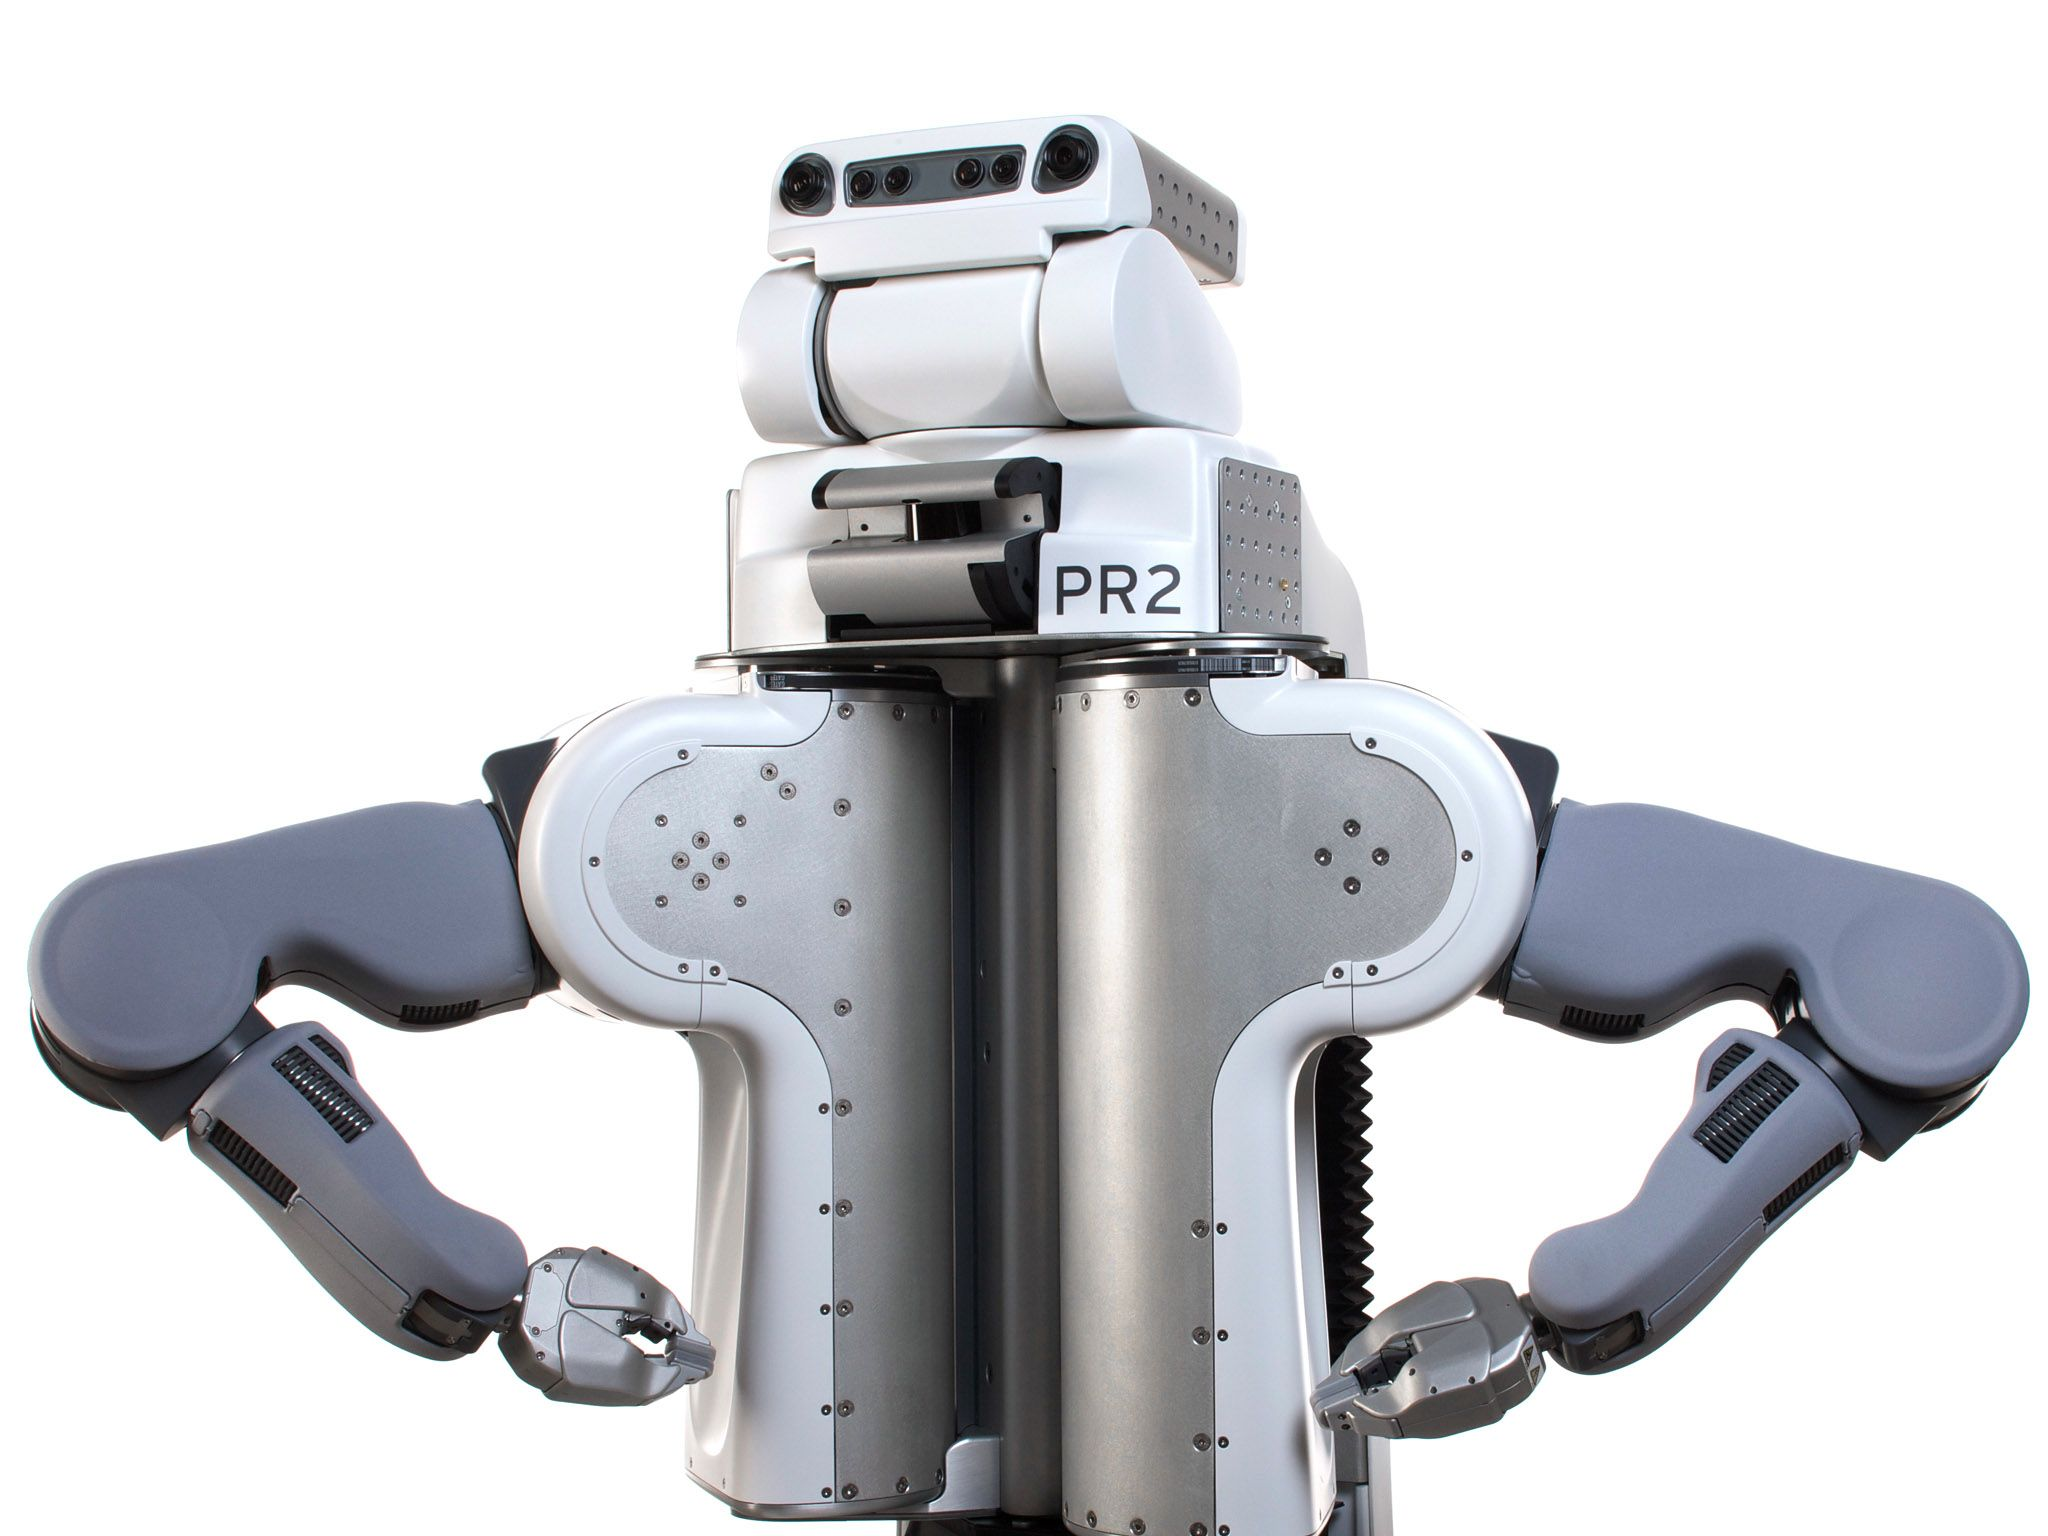
\includegraphics[scale=0.1]{Graphics/pr2.jpg}
    \end{figure}
    \subsection{PyCram}
	\label{sec:pycram}
	\textit{PyCRAM} is a toolbox for designing, implementing and deploying software on autonomous robots. The framework provides various tools and libraries for aiding in robot software development as well as geometric reasoning and fast simulation mechanisms to develop cognition-enabled control programs that achieve high levels of robot autonomy.
    \textit{PyCRAM} is developed in Python with support for the ROS middleware which is used for communication with different software components as well as the robot.
    
    \textit{CRAM} (Cognitive Robot Abstract Machine) \cite{beetz10cram} is a software toolbox for the design, the implementation, and the deployment of cognition-enabled autonomous robots performing everyday manipulation activities.
	\textit{CRAM} equips autonomous robots with lightweight reasoning mechanisms that can infer control decisions rather than requiring the decisions to be pre-programmed. 
	This way \textit{CRAM}-programmed autonomous robots are much more flexible, reliable, and general than control programs that lack such cognitive capabilities. 
	\textit{CRAM} does not require the whole domain to be stated explicitly in an abstract knowledge base. Rather, it grounds symbolic expressions in the knowledge representation into the perception and actuation routines and into the essential data structures of the control programs. 

    \begin{figure}[H]
    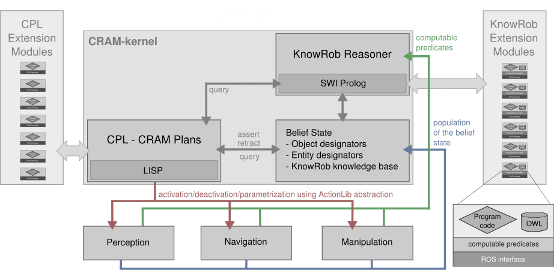
\includegraphics[scale=1.5]{Graphics/cram-language-architecture.png}
	\caption{\textit{CRAM} Language Architecture}
    \end{figure}

	\subsection{PyBullet}
	\label{sec:pybullet}
	\textit{PyBullet}\cite{coumans2021} is an open-source physics engine and 3D simulation library used for robotics, machine learning, and computer graphics research. 
	It offers accurate physics simulation, 3D rendering, robotics support, and seamless integration with machine learning frameworks. 
	With a \textit{Python} API and cross-platform compatibility, it's a versatile tool for simulating complex environments and interactions.
    \section{Knowledge Section: Ontologies and Rules}
    The parameters inferred for various robot actions come from a knowledge base. In the following, the principle of an ontology, as well as the concept of rules, which play a crucial role in parameter inference, will be introduced.
    \subsection{Ontology}
	Ontologies are structured frameworks that provide a formal representation of knowledge within a specific domain. They play a crucial role in knowledge representation, facilitating the organization and sharing of information in a way that is both machine-readable and understandable by humans. 

    \begin{figure}[H]
        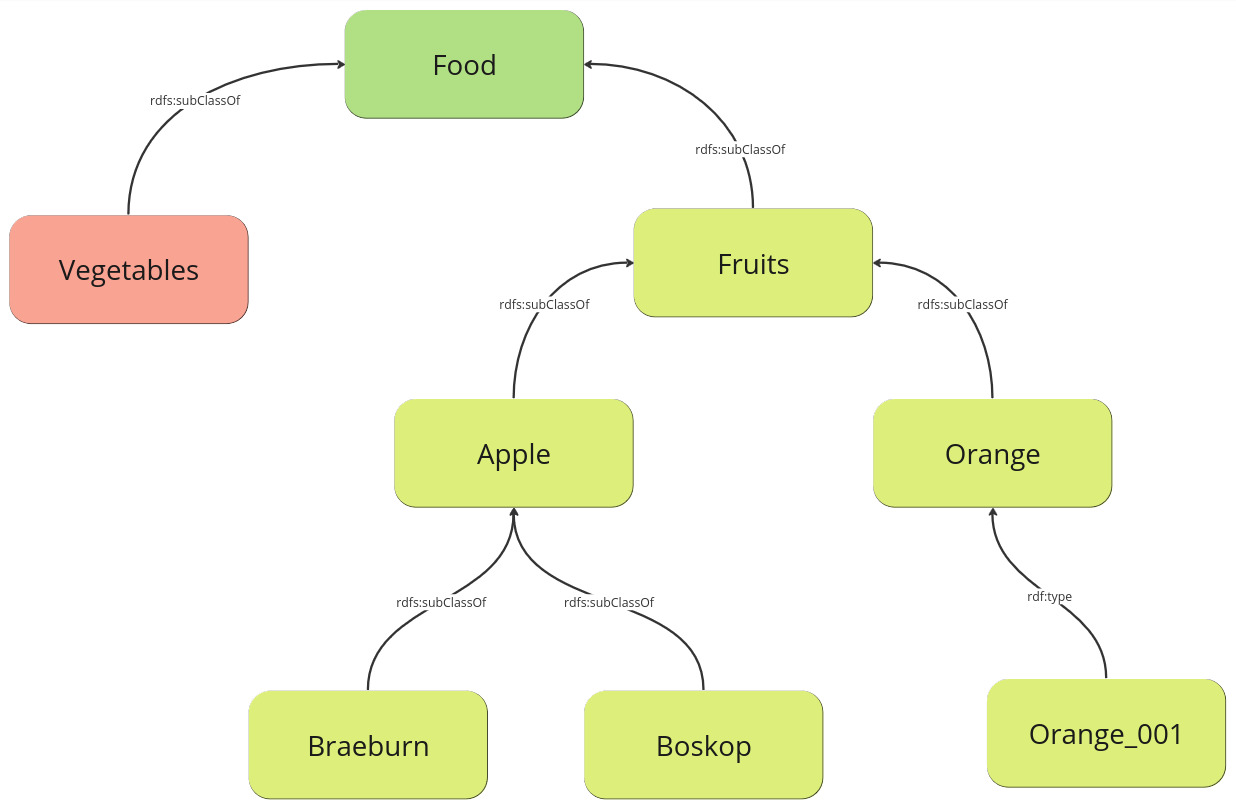
\includegraphics[scale=0.8]{Graphics/ontology.jpg}
		\caption{Ontology example \cite{ontologyexample}}
    \end{figure}
	Key components of ontologies include:

	\begin{itemize}
		\item \textbf{Concepts/Classes}: These represent abstract or concrete entities within a domain. For example, in a medical ontology, \textit{Patient} and \textit{Disease} might be classes.
		\item \textbf{Properties/Roles}: These define the relationships between concepts. For instance, in a social network ontology, \textit{FriendOf} could be a property connecting individuals.
		\item \textbf{Instances/Individuals}: These are specific members or examples of a class. In a geographical ontology, \textit{New York City} and \textit{Paris} could be instances of the class \textit{City}.
		\item \textbf{Axioms}: These are statements that describe the properties and relationships of the entities within the ontology. Axioms help define the logic and rules governing the domain.
		\item \textbf{Hierarchy}: Ontologies often organize concepts into a hierarchy, with more general concepts at the top and more specific ones below. This hierarchical structure aids in categorization and understanding.
		\item \textbf{Inference Rules}: These rules define how new information can be derived from existing information in the ontology. Inferences help systems reason and make deductions based on the knowledge encoded in the ontology.
	\end{itemize}
	We utilize ontologies in knowledge representation and reasoning systems to empower the robot with the ability to comprehend and handle information in a structured fashion for our specific objectives.

	\subsection{SWRL}
	\label{sec:SWRL}
	\textit{SWRL} \cite{Horrocks2004}, which stands for Semantic Web Rule Language, is a rule language that allows users to define rules about the relationships between classes and individuals in ontologies represented in the Web Ontology Language (\textit{OWL}). \textit{SWRL} is part of the W3C's Semantic Web technology stack and is designed to be used in conjunction with \textit{OWL} to express complex relationships and infer new information based on existing knowledge.

	\textit{SWRL} Rules have a specific syntax and consist of two main components:
	\begin{itemize}
		\item \textbf{Antecedent (Body)}: This part of the rule specifies the conditions or constraints that must be satisfied for the rule to be applicable. It describes the current state of the ontology that triggers the rule.
		\item \textbf{Consequent (Head)}: This part defines the actions or inferences that should be taken if the conditions specified in the antecedent are satisfied. It describes the changes or additional information that should be inferred when the rule is triggered.
	\end{itemize}
	\textit{SWRL} supports various built-in predicates and functions, and users can create their own custom rules to suit their specific ontology. Some common elements in \textit{SWRL} rules include:
	\begin{itemize}
		\item \textbf{Individuals}: Refers to specific instances of classes in the ontology.
		\item \textbf{Class and Property Relationships}: Describes relationships between classes and properties in the ontology.
		\item \textbf{Built-in Predicates and Functions:} Includes operations such as arithmetic, string manipulation, and comparison functions that can be used in the rule conditions.
	\end{itemize}
	Here's a simple example of a \textit{SWRL} rule:
	\newline
	$Person(?x) ^ hasChild(?x, ?y) -> Grandparent(?x, ?z) ^ hasChild(?y, ?z)$
	\newline
	In this example:

	If an individual (?x) is a Person and has a child (?y),
	
	Then, infer that the individual (?x) is a Grandparent of another individual (?z), and the child (?y) is the parent of (?z).
	
	\textit{SWRL} rules are useful for expressing complex relationships and constraints within ontologies, enabling automated reasoning systems to make inferences and derive new knowledge from existing data.
	\section{Libraries}
	\label{sec:Libraries}
\subsection{RDFLib}
\label{sec:RDFLib}
\textit{RDFLib} \cite{Krech_RDFLib_2023} is a Python package designed to work with \textit{Resource Description Framework (RDF)} data. RDF is a standard model for data interchange on the web and is used to represent information in the form of subject-predicate-object triples. Key features of the library are:

\begin{itemize}
    \item \textbf{Parsing RDF Data}: \textit{RDFLib} can parse RDF data in various formats such as RDF/XML, N-Triples, Turtle, and more.
    
    \item \textbf{Creating and Modifying RDF Graphs}: It allows you to create and manipulate RDF graphs, which consist of a collection of RDF triples. You can add, remove, or modify triples in the graph.
    
    \item \textbf{Querying RDF Data}: \textit{RDFLib} provides a \textit{SPARQL} query engine, allowing you to perform queries on RDF graphs using the \textit{SPARQL} query language.
    
    \item \textbf{Serializing RDF Data}: You can serialize RDF graphs back into different RDF formats using \textit{RDFLib}, making it easy to store or share RDF data.
    
    \item \textbf{Working with Ontologies}: It supports working with RDF vocabularies and ontologies, enabling the use of predefined classes and properties from existing ontologies like RDF Schema (\textit{RDFS}) or the Web Ontology Language (\textit{OWL}).
    
    \item \textbf{Integration with Semantic Web Tools}: \textit{RDFLib} can be integrated with other Semantic Web tools and frameworks, allowing you to build applications that leverage Semantic Web technologies.
\end{itemize}


	\subsection{Owlready}
	\label{sec:OWLReady}
	One important library used for our implementation is \textit{Owlready} \cite{LAMY201711}. \textit{Owlready} is a \textit{Python} library designed for ontology-oriented programming. It facilitates the development, manipulation, and querying of ontologies using the Web Ontology Language (\textit{OWL}), a standard for representing knowledge in a machine-readable format. \textit{Owlready} simplifies ontology-related tasks by providing a convenient and object-oriented interface for working with \textit{OWL} ontologies in \textit{Python}.

	Key features of the \textit{Owlready} library include:

	\begin{itemize}
		\item \textbf{Object-Oriented Programming (OOP)}: \textit{Owlready} adopts an object-oriented approach, allowing users to interact with ontology entities as Python-objects. This makes it more intuitive for developers familiar with Python's OOP principles.
		\item \textbf{Ontology Loading and Parsing}: The library supports the loading and parsing of \textit{OWL} ontologies, making it easy to access and manipulate ontology data within Python-scripts or applications.
		\item \textbf{Class and Individual Manipulation}: \textit{Owlready} provides functionality for creating, modifying, and querying classes and individuals within an ontology. This allows for dynamic and programmatic management of ontology content.
		\item \textbf{Reasoning Support}: Depending on the version and features, \textit{Owlready} may offer support for reasoning tasks. Reasoning involves deducing implicit information based on the logical relationships defined in the ontology.
		\item \textbf{Integration with \textit{RDFLib}}: \textit{Owlready} may integrate with \textit{RDFLib}, another Python-library commonly used for working with Resource Description Framework (\textit{RDF}) data. This integration enhances the capabilities of handling semantic data.
	\end{itemize}

	\subsection{WikiHow-Instruction-Extraction}
	\label{sec:WikiHow}
	
	\begin{wrapfigure}{r}{0.5\textwidth}
        \centering
        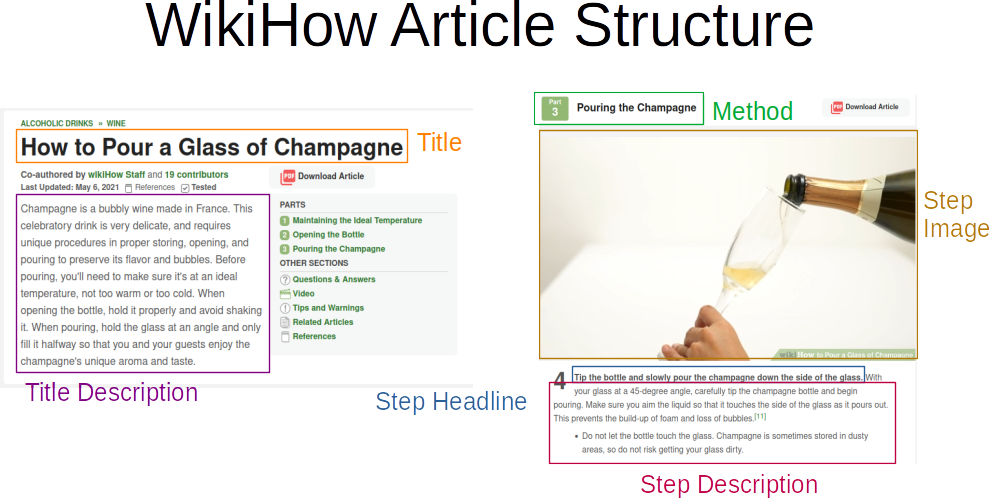
\includegraphics[width=0.48\textwidth]{Graphics/WikiHow Article Structure.png}
    \end{wrapfigure}
	\textit{WikiHow-Instruction-Extraction} \cite{wikihow-extraction}  is an extraction tool, that can collect informations from the WikiHow Corpus. 
	The goal of this tool is to analyse a WikiHow corpus using basic \textit{NLP} techniques to gather information about Everyday tasks like \textit{Pouring}, \textit{Cutting} or \textit{Discarding}. 
	These information should support cognitive robots in understanding and parameterizing these tasks to better handle unknown tasks, working in underspecified environments and handling common task-object combinations.
	Every verb has its own class, in which the verb and the additionally desired hyponyms/synonyms are defined. These verbs serve as keywords for the search in the WikiHow articles. Additionally, various parameters can be set, such as excluding different categories that are not relevant for the search.

\chapter*{Data acquisition}
ToDo:
\begin{itemize}
  \item Aus deutsch ins englische übersetzen.
  \item Beim vorletzten Punkt, die Zutaten Tools und Container besser beschreiben.
  \item Tabelle der Videos vervollständigen.
  \item Code Bild um Stir vervollständigen. 
\end{itemize}
A part of this master's thesis involves creating a knowledge base that includes certain queryable parameters, allowing the robot to perform specific actions. The initial step in building the knowledge base is to gather data. In this chapter, we elaborate on our data acquisition strategy.
\section*{Task variations}
	As our main focus is to represent the knowledge about mixing, first we had to acquire the different types and variations of mixing in order to create a complete Knowldegerepresentation. The first step in acquiring the needed data, was to acknowledge which task varations of mixing are actually important. 
  So we had to analyze the word \textit{Mixing} and its hyponyms. But first we have to ask ourselves What is Mixing?
  \subsection*{What is Mixing?}
  The definition provided by the Oxford Dictionary is as follows: To put together or combine (two or more substances or things) so that the constituents or particles of each are interspersed or diffused more or less evenly among those of the rest; to unite (one or more substances or things) in this manner with another or others; to make a mixture of, to mingle, blend.
  Ultimately, this definition conveys that mixing requires at least two elements or substances, which are then combined (evenly) with each other, resulting in a (new) substance.
  This definition is general and can be applied to various contexts. For our work, the aspect of cooking or mixing different (cooking) ingredients is important. Therefore, we consider some hyponyms of the verb "mixing" irrelevant for our cause and do not take them into account.
  An adapted definition for our work could be: Mixing is the combination of various (cooking) ingredients through different motions in a container.
  
  \subsection*{Mixing hyponyms analysis} 
	Hyponyms are subordered words of a given word, for example one hyponym of mixing could be beating. 
  To conduct this analysis, one can utilize tools from various websites, such as FrameNet and WordNet. These platforms provide users with the ability to search for specific words and obtain various associations for those words, including synonyms, acronyms, or, crucial for our case, hyponyms.	
  \subsubsection*{WikiHow extraction}
  For all those hyponyms, we delegated a WikiHow extraction search which should show us, how many times one of these words occur, in the context of cooking.
	Damit wir die Suche ausführen können definieren wir eine neue Klasse "MixingVerb", welche das Verb Mix, sowie die von uns gefundenen hyponyme und Synonyme enthält.
  \begin{figure}[H]
    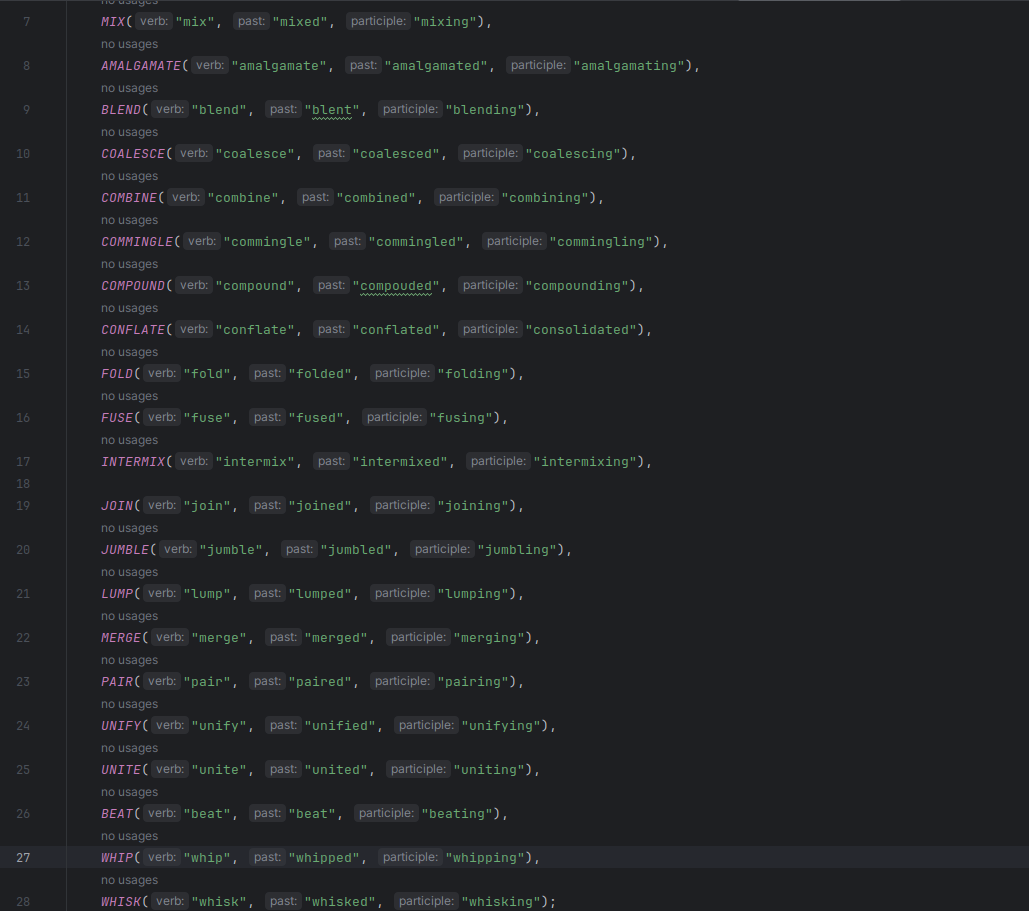
\includegraphics[scale=0.3]{Graphics/MixingVerbClass.png}
    \end{figure}
    IN DEM BILD FEHLT STIRRING
    Since we have now defined the desired verbs that we ultimately want to search for, let's adjust some search parameters. The crucial parameters involve filtering the categories; in our case, we want to focus on mixing in the cooking domain. Therefore, we filter out all articles that do not exist in the Food and Entertaining category.
    \subsubsection*{Hyponyms occurance}
    For each defined verb, a search is initiated to determine how often this verb appears in the WikiHow articles. This is done to ascertain which verbs are ultimately relevant for our implementation and which ones we can exclude, as they are infrequently used in everyday language.
    In the table below the results can be seen.
    \begin{table}[H]
        \centering
        \begin{tabular}{|c|c|}
          \hline
          \textbf{Hyponym} & \textbf{Occurance}  \\
          \hline
          Mix & 5300 \\
          \hline
          Amalgamate & 0 \\
          \hline
          Beat & 956 \\
          \hline
          Blend & 1041 \\
          \hline
          Coalesce & 1 \\
          \hline
          Combining & 3591  \\
          \hline
          Coommingle & 0 \\
          \hline
          Compound & 0 \\
          \hline
          Conflate & 0 \\
          \hline
          Folding & 821 \\
          \hline
          Fuse & 17 \\
          \hline
          Intermix & 0 \\
          \hline
          Join & 53 \\
          \hline
          Jumble & 0 \\
          \hline
          Lump & 7 \\
          \hline
          Merge & 6 \\
          \hline
          Pair & 352 \\
          \hline
          Stir & 6027 \\
          \hline
          Unify & 2 \\
          \hline
          Unite & 2 \\
          \hline
          Whip & 863 \\
          \hline
          Whisk & 2267 \\
          \hline
          
    
        \end{tabular}
        \caption{Mix synoyms/hyponyms occurance}
        \label{tab:example}
      \end{table}
      
  \subsubsection*{Further examination and conclusion}
  This search is ultimately intended to provide us with information on which tasks we want to represent in the knowledge base. Therefore, we decide on certain tasks based on two conditions: frequency and executability. The first condition is easy to understand; tasks that do not occur or occur very rarely are not considered. The second condition relates to the executability of the task in the context of robot movements. Additionally, some tasks with relatively high frequency are also examined more closely, as in English, the past tense is used as an adjective under certain circumstances.

Taking into account the first condition, the following tasks are not considered: Amalgamate, Coalesce, Comingle, Compound, Conflate, Fuse, Intermix, Join, Jumble, Lump, Merge, Unify, and Unite.

The second condition excludes another task: Blend. Blend is mostly used in the context of a blending machine, which is not handled by the robot. Without this machine, the blending execution cannot be performed correctly, so this task is excluded for us.

Upon closer examination, we will also not consider the verb Whip because it is mostly used as an adjective for ingredients, such as whipped cream. This highlights that only the verb Whip has relatively low frequency. The same applies to pair, where the past tense is used to describe a combination of different ingredients, such as wine paired with cheese.

Thus, the tasks we consider are: Mix, Combine, Beat, Fold, Stir, and Whisk.

  \section*{Task analysis and defintion}
  Now that we have selected the tasks, they need to be analyzed to understand the context in which they are ultimately used. Our goal is for the robot to perform these tasks in a manner similar to how a human would. To achieve this, in the next step, we need to closely examine these tasks. It is recommended to analyze videos on WikiHow or other sources where these tasks are presented as activities. The analysis involves observing the movements associated with each task. We present these analyses in tabular form below. The examination includes the task itself, the respective ingredients being processed, the tools used for it, and the container in which the task is carried out.
    \begin{table}[H]
    \centering
    \begin{tabular}{|c|c|c|p{4,5cm}|p{4,5cm}|}
        \hline
        \textbf{Task} & \textbf{Tool} & \textbf{Container} & \textbf{Ingredients} & \textbf{Description} \\
        \hline
        Beating & Whisk & Bowl & Egg yolk (Wet ingredient) & circular, swirling wildly around the bowl \\
        \hline
        Stirring & Whisk & Bowl & Beaten Egg Yolk (Wet), Parmesan(Powder) and Pepper (Powder) & Circular, from the inside to the outside. \\
        \hline
        Stirring & Tongs & Pan & Wet Mixture, Pasta (Solid) and Bacon (Solid) & Diving motions, circular but also straight lines. \\
        \hline
        Whisk & Fork & Bowl & Eggs (Wet) & Circular but also straight, wildly motion. \\
        \hline
        Mixing & Spatula & Pan & Eggs, melted butter (Wet) & Circular, from the inside to the outside, also diving. \\
        \hline
        Folding & Spatula & Pan & cooked eggs in melted butter (Wet) & Gently motion from the outisde to the inside straight, then moving about 90 degree before going to the inside again. \\
        \hline
        Mixing & Spoon & Cup & Dry yeast(Powder), Water (Liquid) & Circular \\
        \hline
        Mixing & Spoon & Bowl & Dry yeast, Water, Flour (Powder), Salt(Powder) & Whirlstorm-like motion. \\
        \hline 
    \end{tabular}
    \caption{Video analysis}
    \label{tab:example}
  \end{table}
NOCH UNVOLLSTÄDNIG

After a thorough analysis of the videos and the information provided in them, we conclude that the executed movement is not only related to the task but also influenced by the ingredients used. However, some tasks are deterministic in the sense that the movement is performed regardless of the specific ingredients.

In the following, we aim to structure the extracted information from the videos and present our findings.

\subsection*{Video analysis conclusion and results}

Based on the extracted information, we conclude that for our goals, the following aspects, in addition to the task, are important and will be further considered:
\begin{itemize}
  \item Ingredients: The ingredients play a crucial role in the movement decision associated with the tasks and will be defined more precisely.
  \item Tools: The tools used may not be decisive in the movement decision, but they are important for the parameters of the robot.????
  \item Container: Das selbe wie oben.
  \item Motions: The motions ultimately represent the movement of the robot for our implementation. These movements are extracted from the videos and defined in alignment with robot motions.
\end{itemize}

\subsubsection*{Ingredients}
Quellen:
\begin{itemize}
  \item https://ceur-ws.org/Vol-2028/paper28.pdf
  \item https://www.freshfarm.org/app/uploads/2020/05/Mixing-Measuring-Wet-and-Dry-Ingredients.pdf
  \item https://www.cookingforengineers.com/article/280/Analyzing-a-Baking-Recipe/print
\end{itemize}
Through the video analysis, we come to the conclusion that the nature of ingredients is important. Primarily, ingredients can be divided into two main categories: Dry and Wet. This division becomes crucial, especially regarding the measurement of quantities for each type of ingredient.

For our case, a somewhat finer categorization of ingredients is necessary to map the various movements sensibly to the given types. In addition to Wet Ingredients, we introduce a new category: Liquid. This corresponds to ingredients falling under Wet Ingredients but with a liquid state, such as milk, water, and oil. This is significant because some movements differ when the given ingredients are Wet or Liquid.

Another category we include is the Solid category. This differs from the Dry category in that it consists of solid components, while we define the Dry category to include powdery substances. The Solid category encompasses foods like vegetables, fruits, and meats. Through these distinctions, we can create a definition refining the ingredient categories.

\textbf{Definition:}
Ingredients are primarily divided into 'Dry' and 'Wet,' with a need for finer differentiation. An abstracted category called 'Liquid' is introduced to encompass liquid states such as milk and water. An additional category, 'Solid,' distinguishes itself from 'Dry' by including solid components like vegetables and meat. These distinctions allow for a precise definition of ingredients, enhancing the analysis of mixing motions in the context of cooking/baking and their representation."
In the initial version, the ingredients we defined are:
\begin{itemize}
  \item Liquid: Milk, Oil, Water, Vinegar, Vanilla Extract, Sauces.
  \item Wet: Egg White, Egg yolk, Butter, Whipped Cream, (mashed fruits?).
  \item Dry: Flour, Salt, Sugar, Baking Soda, Cocoa Powder.
  \item Solid: Onions, Pork, Chicken, Minced meat, Bacon.
\end{itemize}

Hier eventuell nochmal begründen wieso wir die nehmen??.

1. Ansatz: Zutaten aus den Videoanylysen.

2. Ansatz WikiHowExtraction.

\subsubsection*{Tools and Container}
Das kommt von Soma, muss man schauen wie man das beschreiben möchten

\subsubsection*{Motions}
	From this videos we extracted informations about the executed motions. The following motions can be defined:
	\begin{itemize}
		\item \textbf{Circular}: Moving the tool in a defined circular movement in the container, not changing the radius during execution
		\item \textbf{Whirlstorm}: Moving from the inside to the outside of the container with the tool, by circulating in an incremented radius.
		\item \textbf{Folding}: Gently motion, where you start from the outside, moving one straight line to the inner side, then picking the tool up and going to the initial state before moving the tool for about 90 degrees, then going back in a straight line to the inner side of the container again.
		\item \textbf{VerticalCircular}: Imagine a line which can be seen as the diameter of the container, from this line one can define certain regions on which you move the tool circular from side to side. This motion is used by the beating task.
		\item \textbf{CircularDivingToInner}: Starting from the outerside, moving the tool in the container arround its edge for about 270 degrees, before diving to the middle of the container. This motion is used by Tasks where is required to turn the Ingredients over.
	\end{itemize}

\section*{Data Acquision Conclusion}

In the data acquisition phase, our focus was on creating a foundation of the necessary data and information required for a robot to perform various mixing tasks. After identifying the tasks, we were able to analyze videos to examine the movements associated with each task. We concluded that not only the task itself but also the selection of ingredients is crucial for determining the movement.

The ingredients are divided into four different categories, and we were able to define five motions that the robot should perform in a manner consistent with everyday use. In the next chapter, we will present how we intend to represent this knowledge and create a system that enables the robot to know which movement to execute based on a given task and set of ingredients.
\newpage

\chapter{Data Representation}
\label{chap:Data_representation}

In this chapter we are going to introduce our modeled knowledge graph which serves as our \textit{OWL} databasis. We modeled several aspects from the acquired data to cover up the full \textit{Mixing} domain. In other words we definde domain knowledge.

Our main goal is to determine different mixing motions from asserted knowledge, like the given task, the set of ingredients used for mixing and additional knowledge like, which container and which tools are used.
Our knowledge base is not overly abstract but not overly simplified either, the robot doesn't learn how to execute motions, but rather it infers motions and its parameters with asserted knowledge, where the inference rules are kept simple.
By simplyfing the knowledgebase, the robot relies on less asserted knowledge, which can result in a higher success rate.

\section{The Knowledgebase}
We designed a Ontology in which we illustrated our needed classes. 
The Knowledgebase is divided upon the superclasses \textit{Ingredient, DesignedTool, Tasks and Motions }
\begin{figure}[H]
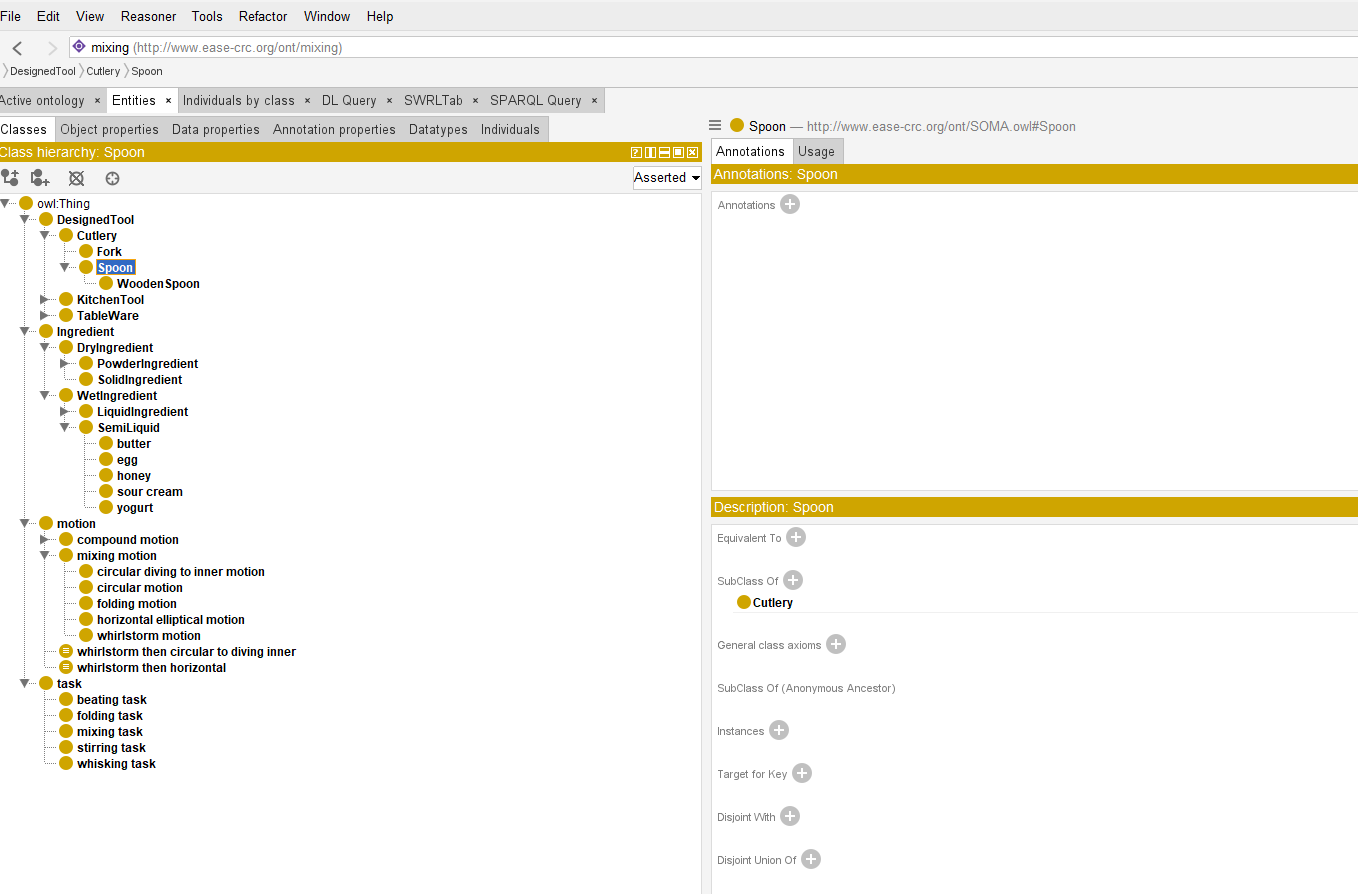
\includegraphics[scale=0.32]{Graphics/ontology05.png}
\caption{modeled Knowledgebase}
\end{figure}

\subsection{Ingredients (outdated)}

\textbf{Definition:}
Ingredients are primarily divided into \textit{Dry} and \textit{Wet}, with a need for finer differentiation. More abstracted categories called \textit{Liquid} and \textit{Semi-Liquid} are introduced to encompass finer states such as milk, egg, butter and water. Also additional categories, \textit{Solid} and \textit{Powder}, distinguishes itself from each other by including solid components like vegetables and meat. These distinctions allow for a precise definition of ingredients, enhancing the analysis of mixing motions in the context of cooking/baking and their representation.

\begin{itemize}
    \item \textit{Liquid: Milk, Oil, Water, Vinegar, Vanilla Extract, Sauces}.
    \item \textit{Semi-Liquid: Egg White, Egg yolk, Butter, Whipped Cream}.
    \item \textit{Powder: Flour, Salt, Sugar, Baking Soda, Cocoa Powder}.
    \item \textit{Solid: Onions, Pork, Chicken, Minced meat, Bacon}.
  \end{itemize}

These subsets are also considered the subclasses for the \textbf{Ingredient} superclass.

By importing the concepts from \textit{FoodOn} (CITE HERE), we not only incorporate the specific ingredient we aim to add to the knowledgebase but also automatically acquire all subclasses of those \textit{FoodOn} concepts, once the ontology is imported into ours. 

This approach applies similarly to \nameref{sec:toolsandcontainers} by leveraging \textit{SOMA}, and it can be extended to ingredients through integration with \textit{FoodOn}.


\subsection{Tools and containers}
\label{sec:toolsandcontainers}

By identifying common occuring containers and tools, 
a generalization can be made and this is where \textit{SOMA} helps. \textit{SOMA-Home} is a taxonomy modelling concepts for a kitchen environment.
Top level concepts from \textit{SOMA-Home} can help us identify specific tools and containers without going through dozens of videos. 
Another advantage is, when \textit{SOMA-Home} is extended with new concepts, those concepts can be easily included into the mixing task procedure. 

The tools can be also divided in multiple categories. \textit{Cutlery} consists of \textit{Fork} and \textit{Spoon}, while \textit{Spoon} also has subclasses like a \textit{Wooden Spoon and Tea Spoon}.
Then we have kitchen tools where we can find different types of \textit{mixers} and \textit{whisks}. Last we got the superclass \textit{Crockery} in which our containers we will be saved, like different \textit{Bowls, Pot and Mugs}.

\subsection{Tasks}
Different tasks will be saved under the \textit{Task} superclass. The tasks consists of \textit{Mixing}, which can be regarded as the umbrela term of all tasks, \textit{Stirring} which is mostly a task that includes a circular motion, \textit{Beating} will be mostly used in context with eggs and other wet ingredients, \textit{Folding} which represents a gentle type of mixing and the last task is \textit{Whisking} which is similar to the beating task.
While some of these tasks have only one motion that can be dervied, like the \textit{Folding} task, we discovered that the others tasks can have multiple motions associated to them. This decision is influenced by the set of ingredients on which the motion will be performed

\subsection{Motions (kein Feedback notwendig, muss grundartig geändert werden.)}
The motions are necessary for the robotic system to know what has to be done?. The motions are inferred from Rules that regards a task component, combined with ingredients.
The motion also contain parameters, which should determine the moving space available for the robotic system. As in the mixing world, most of the container have a circular formed base, our motions are defined with a radius.
The most important parameters are:
\begin{itemize}
    \item Radius Lower Bound: This parameter describes the smallest possible radius for a motion. For example if the used container is a bowl, that has a radius of 10 cm, a radius lower bound of 0.1 would imply that the smallest possible radius on which the robot can perform its motion is 1 cm.
    \item Radius Upper Bound: Similar to the radius lower bound, the upper bound determines the maximum radius on which the robot can execute motions.
\end{itemize}
Our implemented motions are:
\begin{itemize}
    \item Circular Motion: A circular motion is a motion defined on a circular with a constant radius. This motion has an equal lower und upper bound radius to keep the radius of the motion constant.  \newline HIER BILD
    \item Whirlstorm Motion: The Whirlstorm motion covers multiple parts of the container, the motion starts on the center of the container and increments its radius until it reaches the radius upper bound parameter, before turning back to the center. \newline HIER BILD
    \item Folding Motion: Folding is a special motion which is mostly used in the context of the folding task. The motion's goal is to mix the ingredients gently without overmixing the mixture. The motion starts on a point on the circle with the radius of the upper bound parameter, from there the motion draws a straight line to the middle point of the container, then getting back to the start point, next the tool will be moved 90 degrees on the defined circle and it moves back to the middle, this motion is repeteadet 4 times, and then you move the tool 20 degrees to cover all of the ingredients before starting the cycle again. \newline HIER BILD
    \item Vertical Circular Motion: The last motion can also be seen as the most difficult one. The main idea of this motion is to `wildly` mix the ingredients. Beschreibung fehlt, Bild hier rein.
\end{itemize}

\section{Rules}
In order to infer the right motion based on the ingredients and task input, rules have to be defined. This rules are \nameref{sec:SWRL}-rules.
In this section we want to illustrate the inference on a high level.
The rules can be thoguht as if conditions, which will then result in a motion, 
for example, if we regard the combination of the task \textit{Mixing} and the ingredient type \textit{Liquid}, we infer the motion \textit{Whirlstormmotion}. 
This can be done for every task and ingredient combination. 
The inference can be illustrated with decision trees which will be shown in the following section for every task and ingredient type combination available. 

\subsection{Mixing}
\begin{figure}[H]
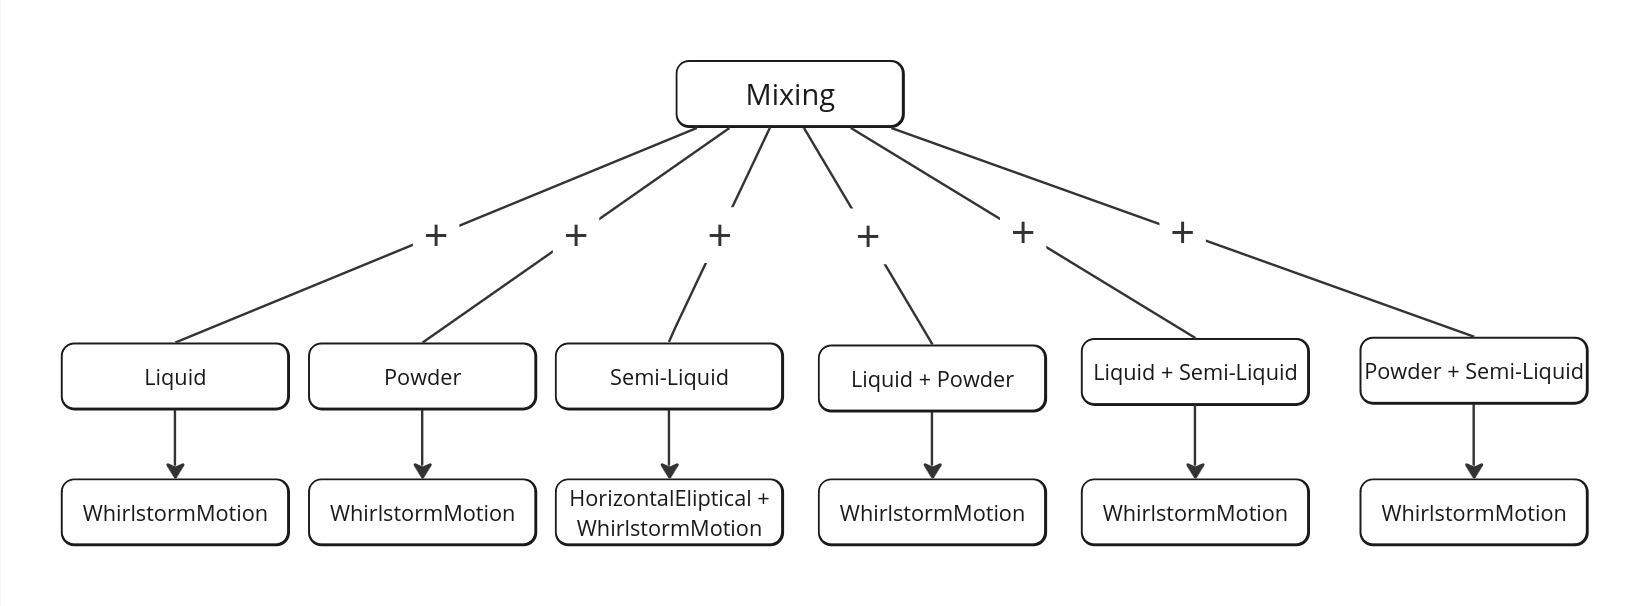
\includegraphics[scale=0.18]{Graphics/MixingDecisionTree.jpg}
\caption{Mixing decision tree}
\end{figure}
\textbf{Definition:} In the context of baking or cooking, a mixing task refers to the process of combining multiple ingredients thoroughly to create a homogeneous mixture. The goal is to distribute the ingredients evenly, ensuring that each component contributes to the overall texture, flavor, and consistency of the final dish or baked good. Mixing is a fundamental step in many recipes and is essential for achieving a balanced and cohesive result (Quelle).


As can be seen from the illustration, the mixing task can primarily be mapped to the Whirlstorm motion. This is not surprising when considering the definition, as this motion results in the uniform distribution of all ingredients in the container.
\subsection{Stirring}
\begin{figure}[H]
    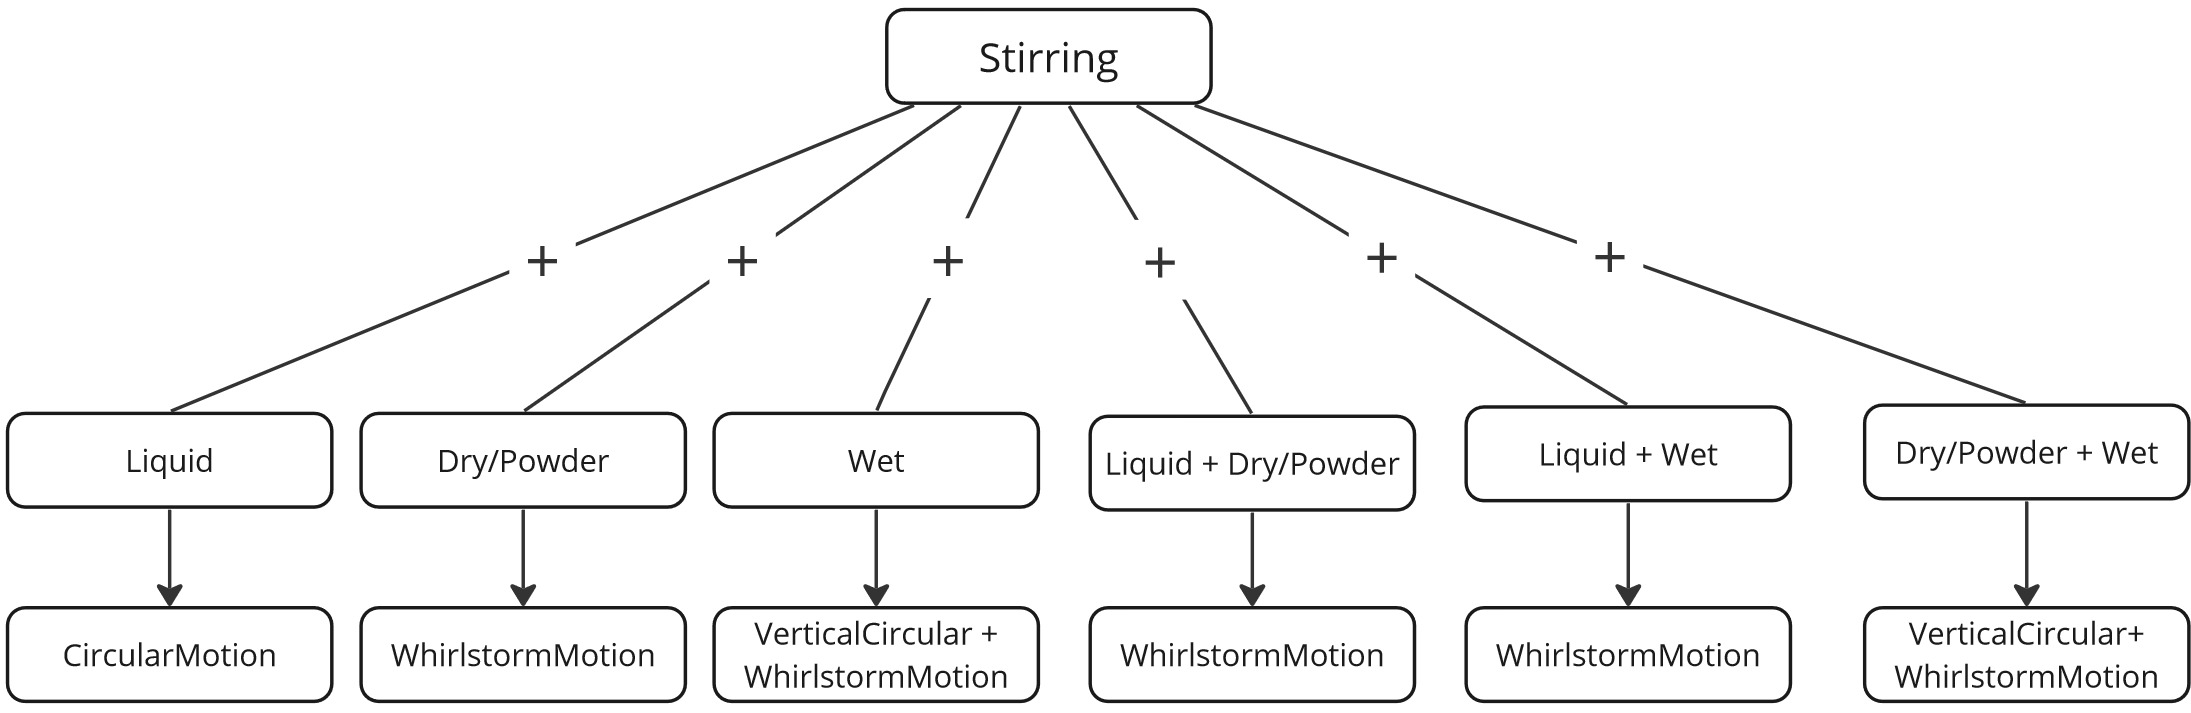
\includegraphics[scale=0.18]{Graphics/StirringDeisionTree.jpg}
    \end{figure}
\textbf{Definition:}
In the context of baking or cooking, a stirring task involves using a utensil, such as a spoon, spatula, or whisk, to agitate and circulate the ingredients within a mixture. The purpose of stirring is to achieve a uniform distribution of ingredients

In comparison to \textit{Mixing}, the \textit{Stirring} task, depending on the ingredients, maps to a broader range of motions. In addition to the \textit{WhirlstormMotion}, the \textit{Circular Motion} is used here for the first time. This is particularly important when considering the \textit{Stirring} task with the ingredient type \textit{Liquid}, as one does not want the ingredients to be whirled, as would be the case with the \textit{Whirlstorm Motion}, but rather just stirred.
\subsection{Beating}
\begin{figure}[H]
    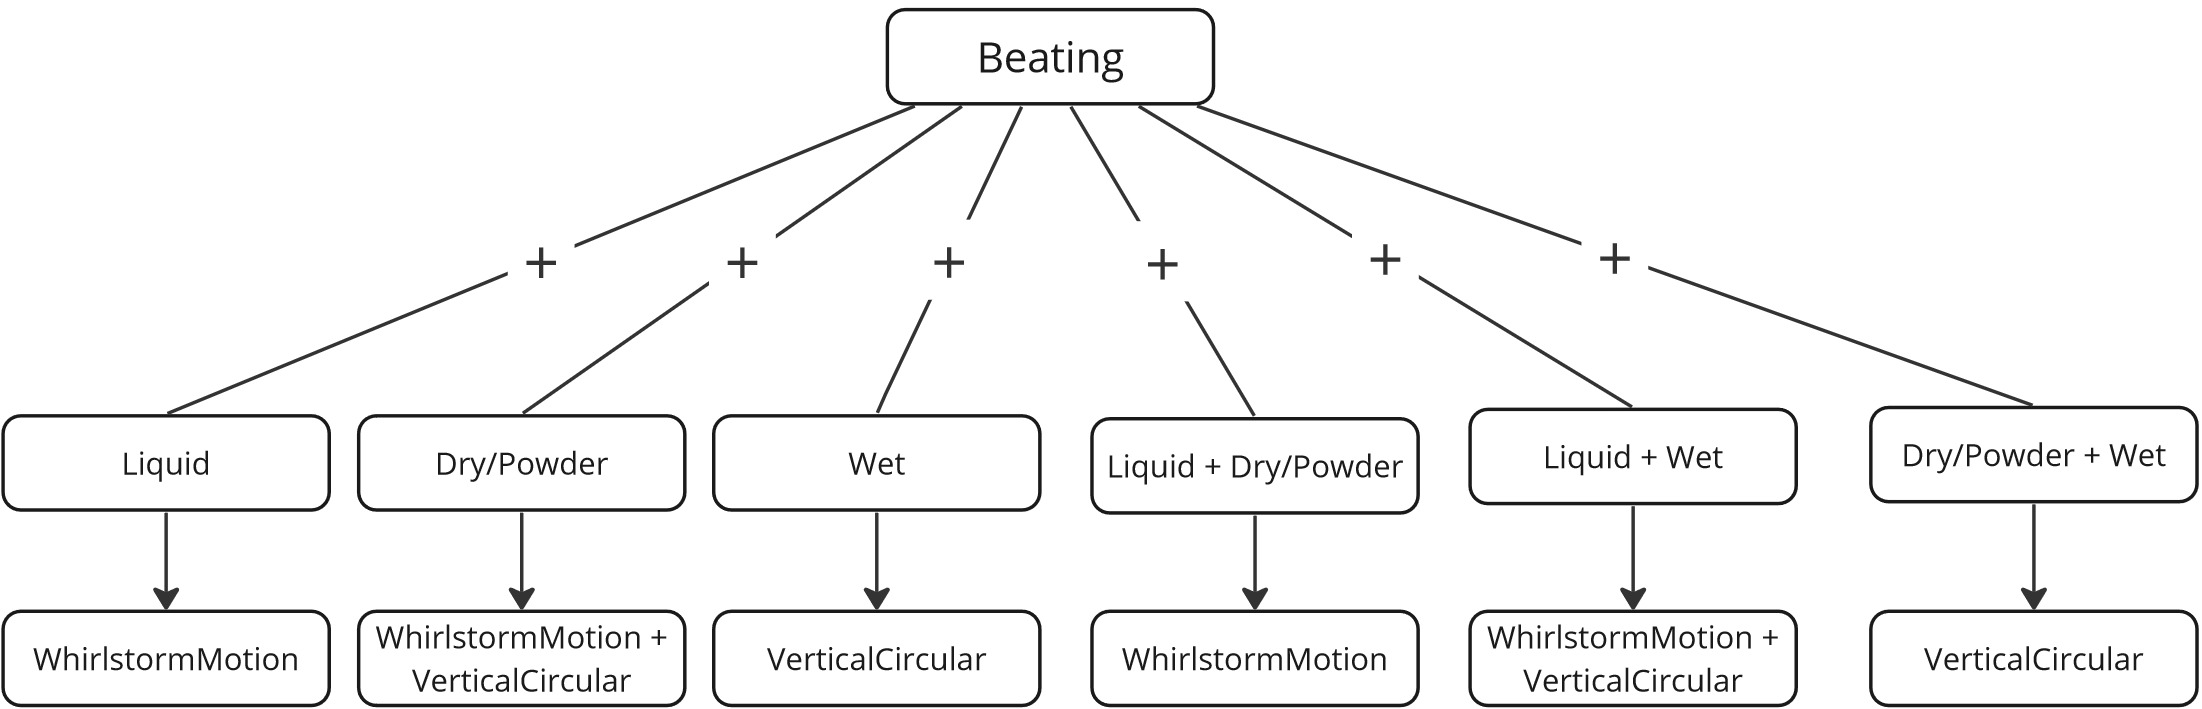
\includegraphics[scale=0.18]{Graphics/BeatingDecisionTree.jpg}
    \end{figure}
\textbf{Definition:}
In the context of baking and cooking, a "beating" task refers to the process of vigorously stirring or mixing ingredients to achieve a specific texture or consistency. Beating is often done to incorporate air into the mixture, create smooth and uniform blends, or alter the physical properties of certain ingredients.

In addition to the Whirlstorm Motion, the Horizontal Eliptic Motion also predominates here. This can be derived from the definition as well, as this motion requires a wild mixing style, to which the Horizontal Eliptic Motion aligns.
\subsection{Whisking}
\begin{figure}[H]
    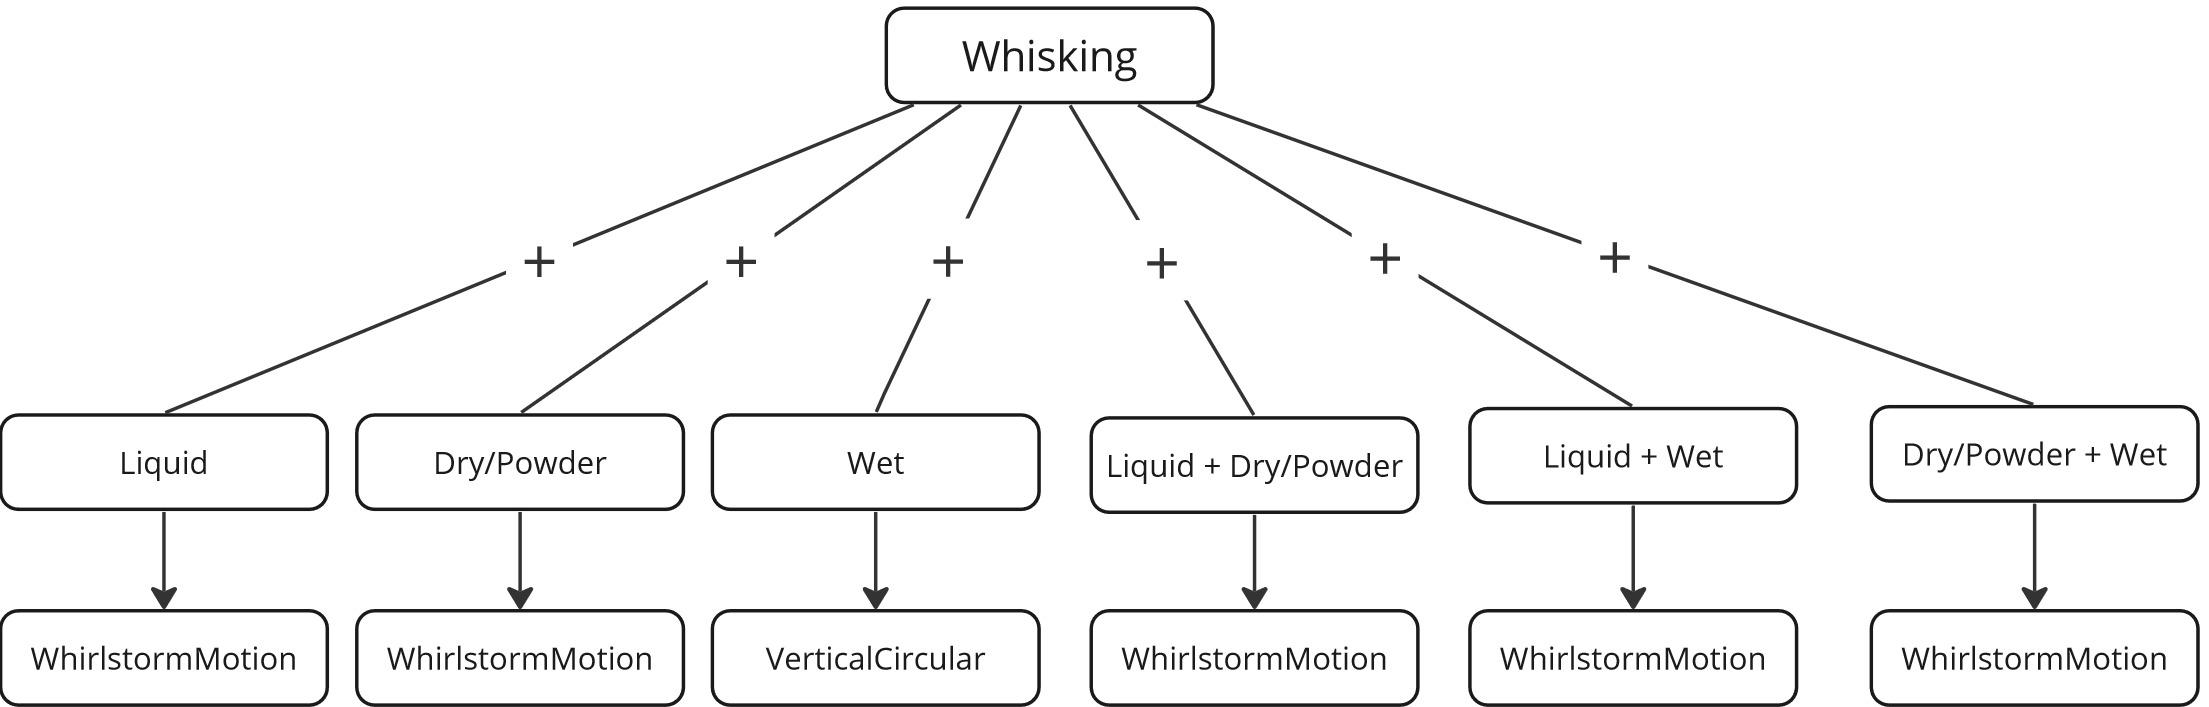
\includegraphics[scale=0.18]{Graphics/WhiskingDecisionTree.jpg}
    \end{figure}
\textbf{Definion:}In the context of baking and cooking, a "whisking" task involves using a kitchen utensil called a whisk to mix, blend, or beat ingredients. A whisk typically consists of wire loops or a coil attached to a handle, and it is designed to incorporate air into mixtures, break up clumps, and create a smooth and uniform texture.

\subsection{Folding}
\begin{figure}[H]
    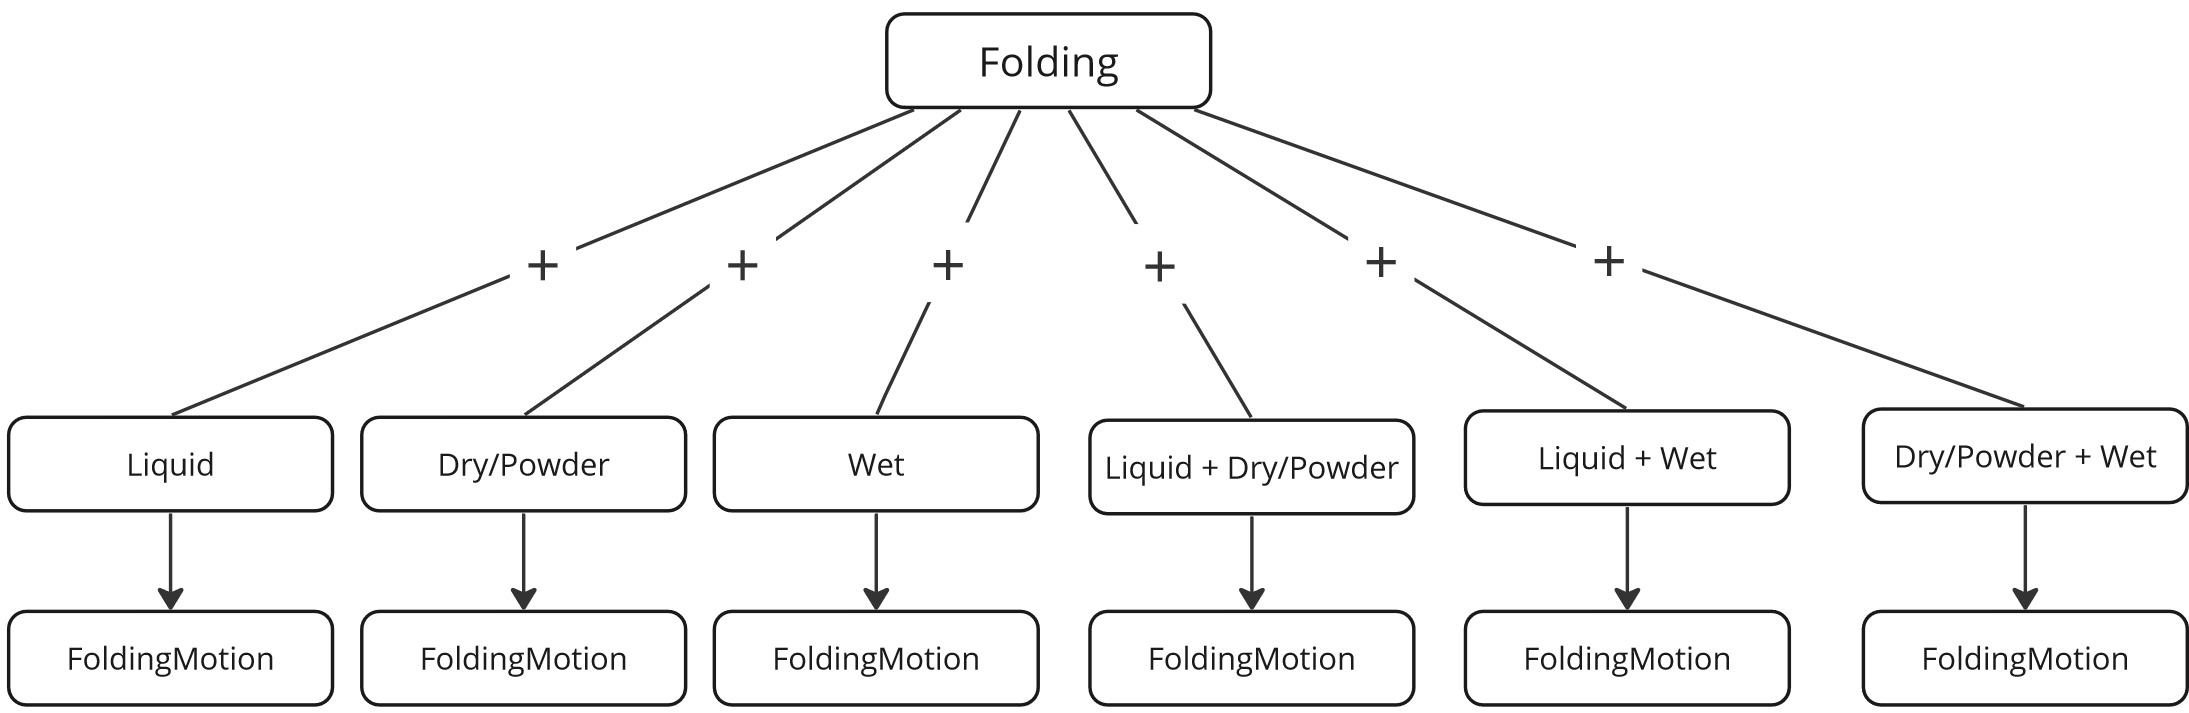
\includegraphics[scale=0.18]{Graphics/FoldingDecisionTree.jpg}
    \end{figure}
\textbf{Definition:}
In the context of baking and cooking, a "folding" task refers to a gentle mixing technique used to incorporate ingredients without deflating or destroying the air bubbles that have been created. Folding is often employed when combining a lighter mixture (such as whipped cream or beaten egg whites) with a denser one (such as a batter or a heavier mixture). The goal is to maintain the desired texture, lightness, or fluffiness in the final dish.

Theoretically, we wouldn't need to graphically represent the Folding Task since each task and ingredient combination maps to a single motion, the Folding Motion. The graphic was nevertheless included for completeness. The Folding Task requires a specific movement that does not remove the air in the mixture, and any other movement would fail.
\section{How to expand the Knowledgebase}

\chapter*{Simulation}

In diesem Kapitel stellen wir die Simulation vor, indem der Agent die definierten Motions ausführen kann und dadurch als Proof of Concept dient. 
Zunächst werden wir die Simulationsumgebung Bulletworld vorstellen, gefolgt von einigen Beispielsaktionen die dort ausgeführt werden können.
Anschließend zeigen wir, wie die Parameter über Queries inferriert werden und mit der Visulasierung der Motions zeigen wir, dass die von uns definierten Motions + Parameter vom Roboter in der Simulation ausgeführt werden können.

\section*{Simulation Environment}

Die Simulationsumgebung ist Bulletworld, welche als Simulationsumgebung für das Framework PyCram dient. Dies ist sehr günstig, denn somit können die in PyCram definierten Aktionen direkt simuliert werden und müssen nicht extra geportet werden. Als Schnittstelle zu den Roboter wird ROS1 genutzt, um mit den Joints zu kommunizieren. Dies geschieht über RosNodes, darüber kann man Informationen über den Zustand der Joints (oder andere Komponente) erhalten, sowie mit diesen Komponenten kommunizieren um Aktionen zu befehlen.

Der für unsere Zwecken genutzten Roboter ist der PR2, dieser ist als Modell schon in der Bulletworld implementiert und ist für unser Fall geeignet, da für die Motions, 2 Arme benötigt werden, eins um die jeweiligen Container zu halten und den anderen Arm, um das Tool, welches für die Aktionen genutzt wird, bewegt wird.

Die Umgebung, welche für unsere definierten Aktionen genutzt wird, ist eine Küche, die Möbel besteht aus einem Tisch, worauf die genutzten Container platziert werden und die Motions dementsprechend ausgeführt werden, sowie weitere Küchenmöbel, welche für unsere Fälle nicht relevant sind.
BILDER KÜCHESIMULATION

Die von uns genutzten Objekte sind:
\begin{itemize}
	\item Container: Bowl (klein und groß), Pfanne, Topf und Tasse. BILDER
	\item Tools: Whisk, Löffel (klein und groß), Holzlöffel. BILDER
\end{itemize}

PyCram bietet schon eine betrachtliche Anzahl an implementierten Aktionen, womit der Roboter manevriert werden kann. Unter diesen Aktionen befinden sich notwendige Navigationaktionen, sowie manipulative Aktionen wie Greifen und Platzieren. Außerdem bietet PyCram schon Schnittstellen bereit womit die Joints des Roboters bewegt werden können, diese Funktionen heißen dann zum Beispiel moveTorso().
BILDER CODE FUNKtIONEN

\section*{HIER STELLEN WIR UNSERE MOTIONS VOR}
Hier Vanessa fragen, wie wir ihre Motion referenzieren sollen, einfahc sagen es war vorhanden oder es detaillierten angeben?

\section*{Simulation to RealWorld gap}
\begin{itemize}
	\item Big Problem: Uncertaininty
	\item Perception Solution as first approach: RoboKudo
	\item Data acquisition: Blenderproc
	\item Model Training: YoloV8
	\item Results showing the real world Perception.
\end{itemize}

\section{Evaluation}
\label{sec:evaluation}
In this section, we aim to present our implemented/adapted motions as a proof of concept. We consider all possible combinations of tasks and ingredients applied to every possible combination of tools and containers. Each task will showcase only one example in this chapter, with the rest available and more detailed in the appendix. The respective task trees are located in Chapter \nameref{chap:Data_representation}, which illustrates which motions result from combinations of tasks and ingredients.

Through this evaluation, we aim to demonstrate that the knowledge base we have developed can aid in inferring dynamic motions along with parameters that adapt to both the tool and container. Our parameters are relative to the dimensions of the container, specifically the radius within which the motion is executed, as well as the dimensions of the tools used to execute the motion. It is crucial that the motion in the simulation does not exceed the predetermined dimensions, as this could have potentially serious consequences when applied in the real world.
\subsection*{Mixing Task}

\begin{table}[H]
    \centering
    \begin{tabular}{|c|c|c|c|c|}
      \hline
      \textbf{Nr.} & \textbf{Ingredients} & \textbf{Tool} & \textbf{Container} & \textbf{Inferred Motion}  \\
      \hline
      1 & Liquid & WoodenSpoon & Salad Bowl & Whirlstorm Motion \\
      \hline
      2 & Powder & WoodenSpoon & Salad Bowl & Whirlstorm Motion \\
      \hline
      3 & Liquid + Dry & WoodenSpoon & Salad Bowl & Whirlstorm Motion \\
      \hline
      4 & Liquid + SemiLiquid & WoodenSpoon & Salad Bowl & Whirlstorm Motion \\
      \hline
      5 & Powder + Wet & WoodenSpoon & Salad Bowl & Whirlstorm Motion \\
      \hline
      6 & SemiLiquid & WoodenSpoon & Salad Bowl & VerticalCircular + 
      \\ & & &  & Whirlstorm Motion \\
      \hline
    \end{tabular}
    \caption{Mixing Task}
    \label{tab:mixingtask}
  \end{table}

\begin{itemize}
  \item Inferred Parameters for \textbf{1-5}: 
   \begin{lstlisting}
    => radius_lower_bound_relative = 0.0, 
    radius_upper_bound_relative = 0.7
  \end{lstlisting}
  \item Inferred Parameters for \textbf{6}:
  \begin{lstlisting}
    => radius_lower_bound_relative = 0.0, 
    radius_upper_bound_relative = 0.7,
    ellipse_shift = 0.04
  \end{lstlisting}
\end{itemize}

\begin{figure}[H]
  \centering
  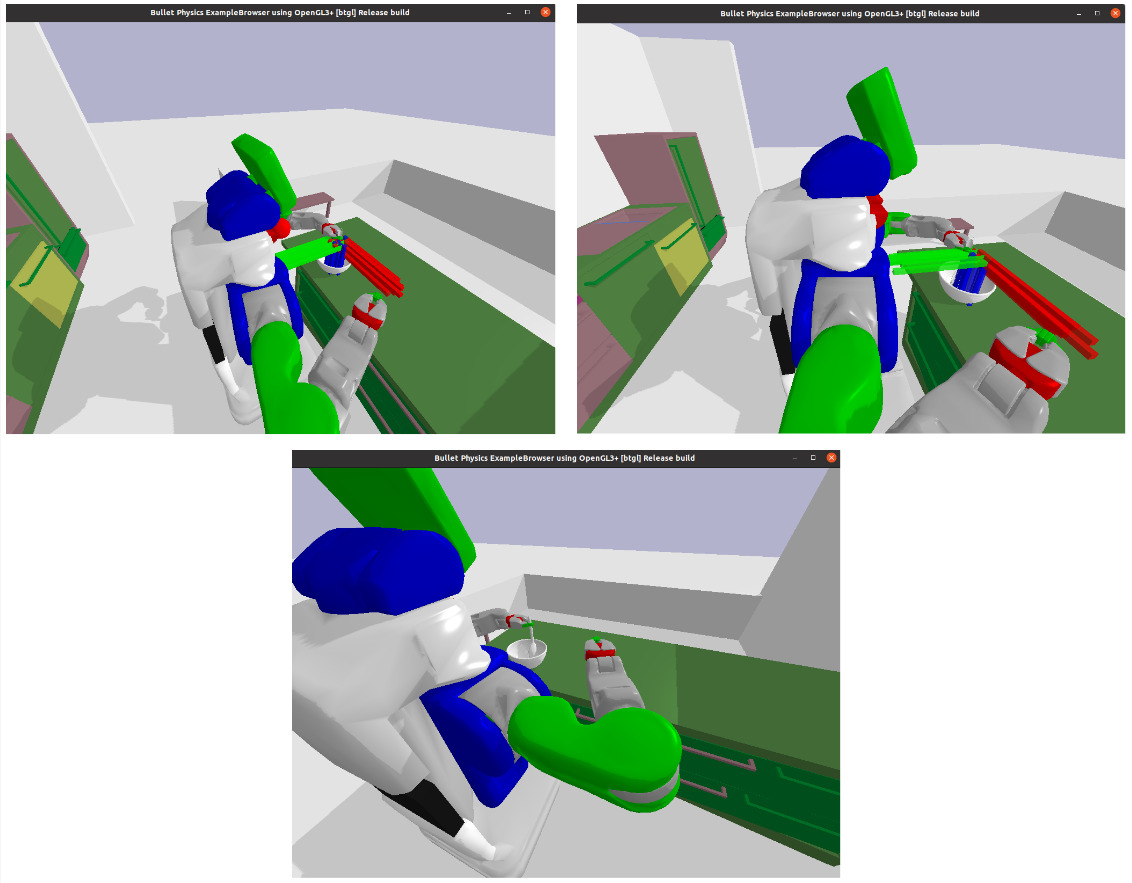
\includegraphics[scale=0.35]{Graphics/mixing_evaluation.jpg}
  \caption{Inferred \textit{Mixing} Motions}
  \label{fig:mixingverb WikiHow}
\end{figure}

\subsection*{Beating Task}

\begin{table}[H]
  \centering
  \begin{tabular}{|c|c|c|c|c|}
    \hline
    \textbf{Nr.} & \textbf{Ingredients} & \textbf{Tool} & \textbf{Container} & \textbf{Inferred Motion}  \\
    \hline
    1 & Liquid & Fork & Salad Bowl & Whirlstorm Motion \\
    \hline
    2 & Powder & Fork & Salad Bowl & Whirlstorm Motion +
    \\ & & &  & Horizontal Eliptical Motion \\
    \hline
    3 & Liquid + Powder & Fork & Salad Bowl & Whirlstorm Motion \\
    \hline
    4 & Liquid + SemiLiquid & Fork & Salad Bowl & Whirlstorm Motion +
    \\ & & &  & Horizontal Eliptical Motion \\
    \hline
    5 & Powder + SemiLiquid & Fork & Salad Bowl & Horizontal Eliptical 
    \\ & & &  & Motion \\
    
    \hline
    6 & SemiLiquid & Fork & Salad Bowl & Horizontal Eliptical 
    \\ & & &  & Motion \\
    \hline
  \end{tabular}
  \caption{Beating Task}
  \label{tab:mixingtask}
\end{table}

\begin{figure}[H]
  \centering
  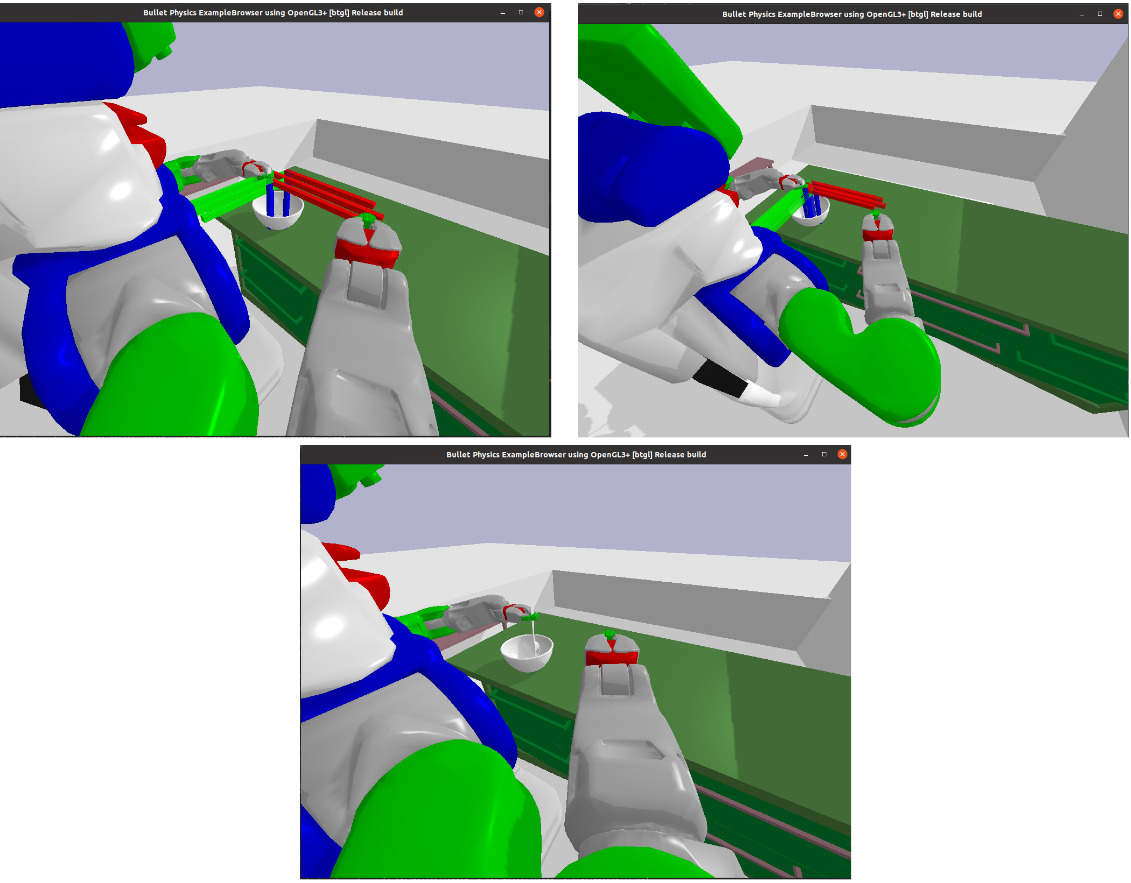
\includegraphics[scale=0.33]{Graphics/beating_evaluation.jpg}
  \caption{Inferred \textit{Beating} Motions}
  \label{fig:mixingverb WikiHow}
\end{figure}


\begin{itemize}
\item Inferred Parameters for \textbf{1,3}: 
 \begin{lstlisting}
  => radius_lower_bound_relative = 0.0, 
  radius_upper_bound_relative = 0.7
\end{lstlisting}
\item Inferred Parameters for \textbf{2,4,5,6}:
\begin{lstlisting}
  => radius_lower_bound_relative = 0.0, 
  radius_upper_bound_relative = 0.7,
  ellipse_shift = 0.04
\end{lstlisting}
\end{itemize}

\subsection*{Stirring Task}

\begin{table}[H]
  \centering
  \begin{tabular}{|c|c|c|c|c|}
    \hline
    \textbf{Nr.} & \textbf{Ingredients} & \textbf{Tool} & \textbf{Container} & \textbf{Inferred Motion}  \\
    \hline
    1 & Liquid & Wooden Spoon & Pot & Circular Motion \\
    \hline
    2 & Powder & Wooden Spoon & Pot & Whirlstorm Motion\\
    \hline
    3 & Liquid + Powder & Wooden Spoon & Pot & Whirlstorm Motion \\
    \hline
    4 & Liquid + Semi-Liquid & Wooden Spoon & Pot & Whirlstorm Motion \\
    \hline
    5 & Powder + Semi-Liquid & Wooden Spoon & Pot & Whirlstorm Motion +
    \\ & & &  &Horizontal Eliptical Motion \\
    \hline
    6 & Semi-Liquid & Wooden Spoon & Pot & Whirlstorm Motion +
    \\ & & &  &Horizontal Eliptical Motion \\
    \hline
  \end{tabular}
  \caption{Stirring Task}
  \label{tab:mixingtask}
\end{table}

\begin{figure}[H]
  \centering
  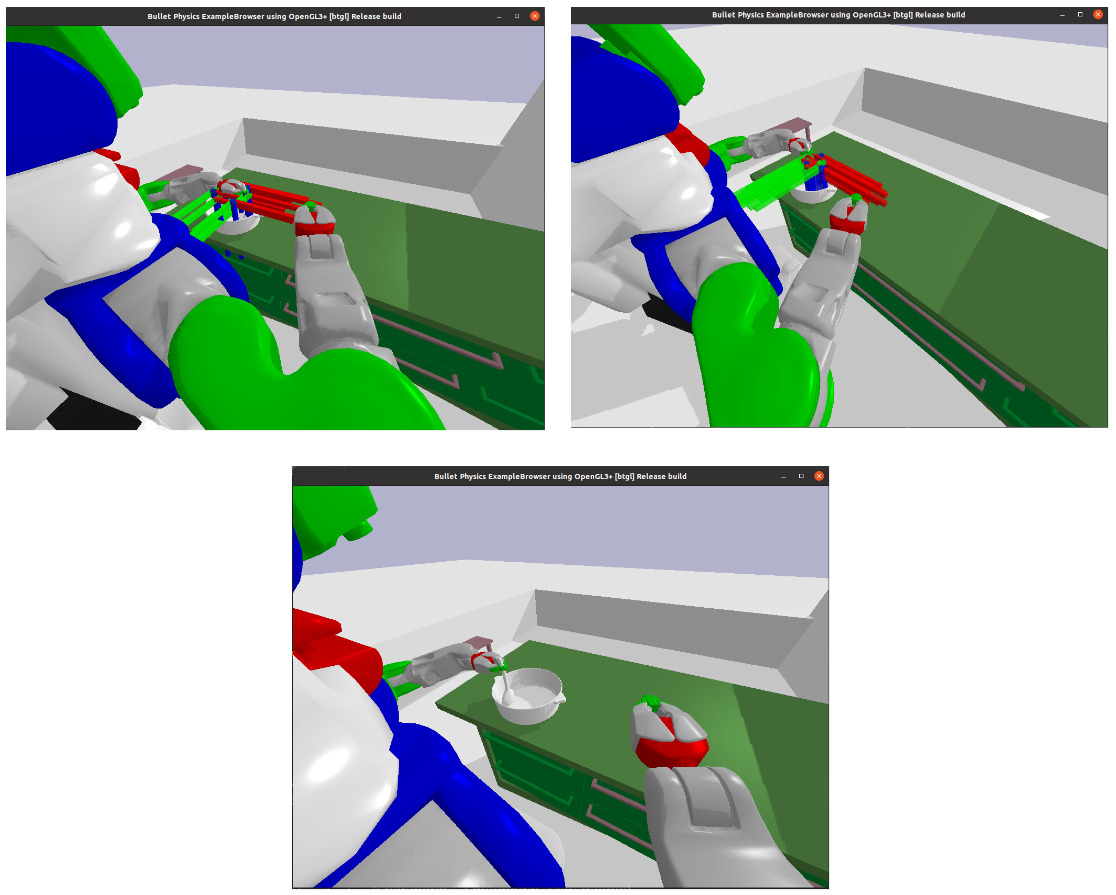
\includegraphics[scale=0.36]{Graphics/stirring_evaluation.jpg}
  \caption{Inferred \textit{Stirring} Motions}
  \label{fig:mixingverb WikiHow}
\end{figure}

\begin{itemize}
\item Inferred Parameters for \textbf{1}: 
 \begin{lstlisting}
  => radius_lower_bound_relative = 0.7, 
  radius_upper_bound_relative = 0.8
\end{lstlisting}
\item Inferred Parameters for \textbf{2,3,4}:
\begin{lstlisting}
  => radius_lower_bound_relative = 0.0, 
  radius_upper_bound_relative = 0.7,
  ellipse_shift = 0.04
\end{lstlisting}
\item Inferred Parameters for \textbf{5,6}:
\begin{lstlisting}
  => radius_lower_bound_relative = 0.0, 
  radius_upper_bound_relative = 0.7,
  ellipse_shift = 0.04
\end{lstlisting}
\end{itemize}

\subsection*{Whisking Task}

\begin{table}[H]
  \centering
  \begin{tabular}{|c|c|c|c|c|}
    \hline
    \textbf{Nr.} & \textbf{Ingredients} & \textbf{Tool} & \textbf{Container} & \textbf{Inferred Motion}  \\
    \hline
    1 & Liquid & Whisk & Bowl & Whirlstorm Motion \\
    \hline
    2 & Powder & Whisk & Bowl & Whirlstorm Motion\\
    \hline
    3 & Liquid + Powder & Whisk & Bowl & Whirlstorm Motion \\
    \hline
    4 & Liquid + Semi-Liquid & Whisk & Bowl & Whirlstorm Motion \\
    \hline
    5 & Powder + Semi-Liquid & Whisk & Bowl & Whirlstorm Motion \\
    \hline
    6 & Semi-Liquid & Whisk & Bowl & Horizontal
    \\ & & &  &Eliptical Motion \\
    \hline
  \end{tabular}
  \caption{Whisking Task}
  \label{tab:mixingtask}
\end{table}

\begin{figure}[H]
  \centering
  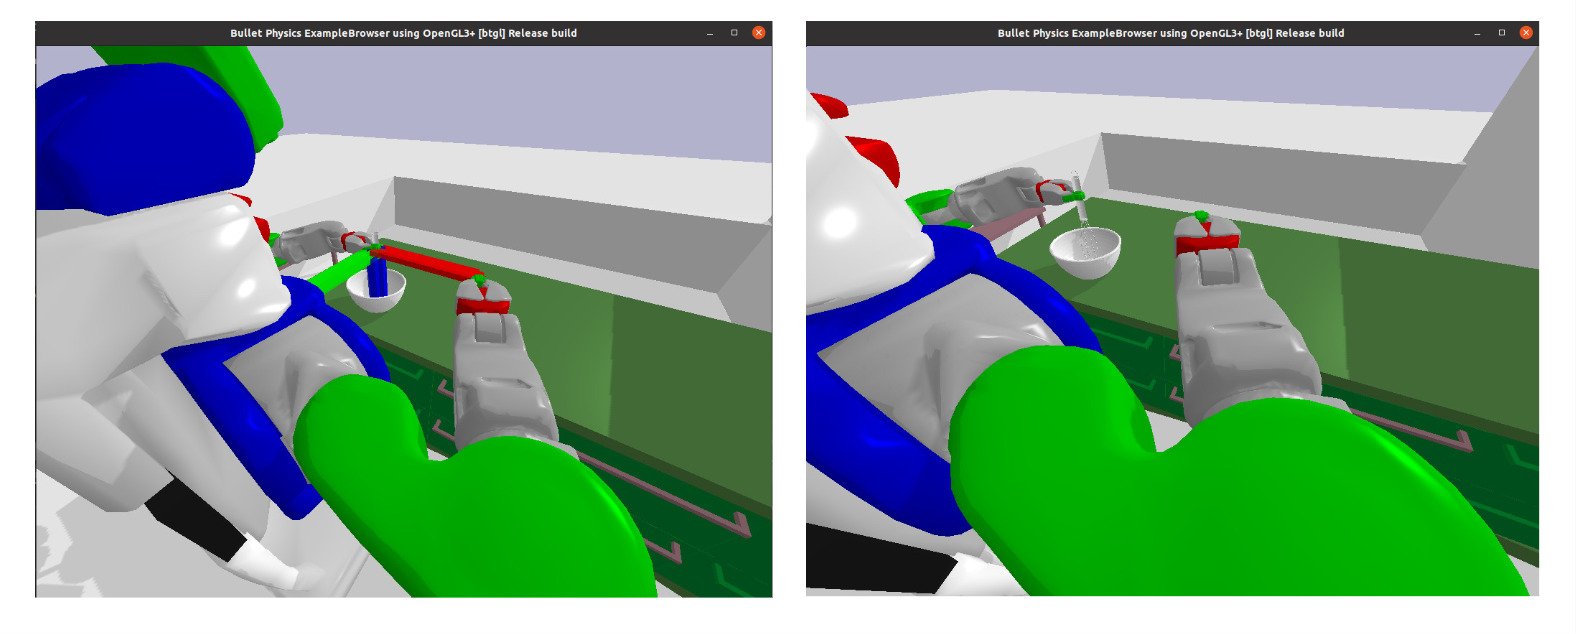
\includegraphics[scale=0.25]{Graphics/whisking_evaluation.jpg}
  \caption{Inferred \textit{Whisking} Motions}
  \label{fig:mixingverb WikiHow}
\end{figure}

\begin{itemize}
\item Inferred Parameters for \textbf{1,2,3,4,5}: 
 \begin{lstlisting}
  => radius_lower_bound_relative = 0.0, 
  radius_upper_bound_relative = 0.7
\end{lstlisting}
\item Inferred Parameters for \textbf{6}:
\begin{lstlisting}
  => radius_lower_bound_relative = 0.0, 
  radius_upper_bound_relative = 0.7,
  ellipse_shift = 0.04
\end{lstlisting}
\end{itemize}

\subsection*{Folding Task}
\begin{table}[H]
  \centering
  \begin{tabular}{|c|c|c|c|c|}
    \hline
    \textbf{Nr.} & \textbf{Ingredients} & \textbf{Tool} & \textbf{Container} & \textbf{Inferred Motion}  \\
    \hline
    1 & Liquid & Fork & Pot & Folding Motion \\
    \hline
    2 & Powder & Fork & Pot & Folding Motion \\
    \hline
    3 & Liquid + Powder & Fork & Pot & Folding Motion \\
    \hline
    4 & Liquid + Semi-Liquid & Fork & Pot & Folding Motion \\
    \hline
    5 & Powder + Semi-Liquid & Fork & Pot & Folding Motion \\
    \hline
    6 & Semi-Liquid & Fork & Pot & Folding Motion \\
    \hline
  \end{tabular}
  \caption{Folding Task}
  \label{tab:mixingtask}
\end{table}

\begin{figure}[H]
  \centering
  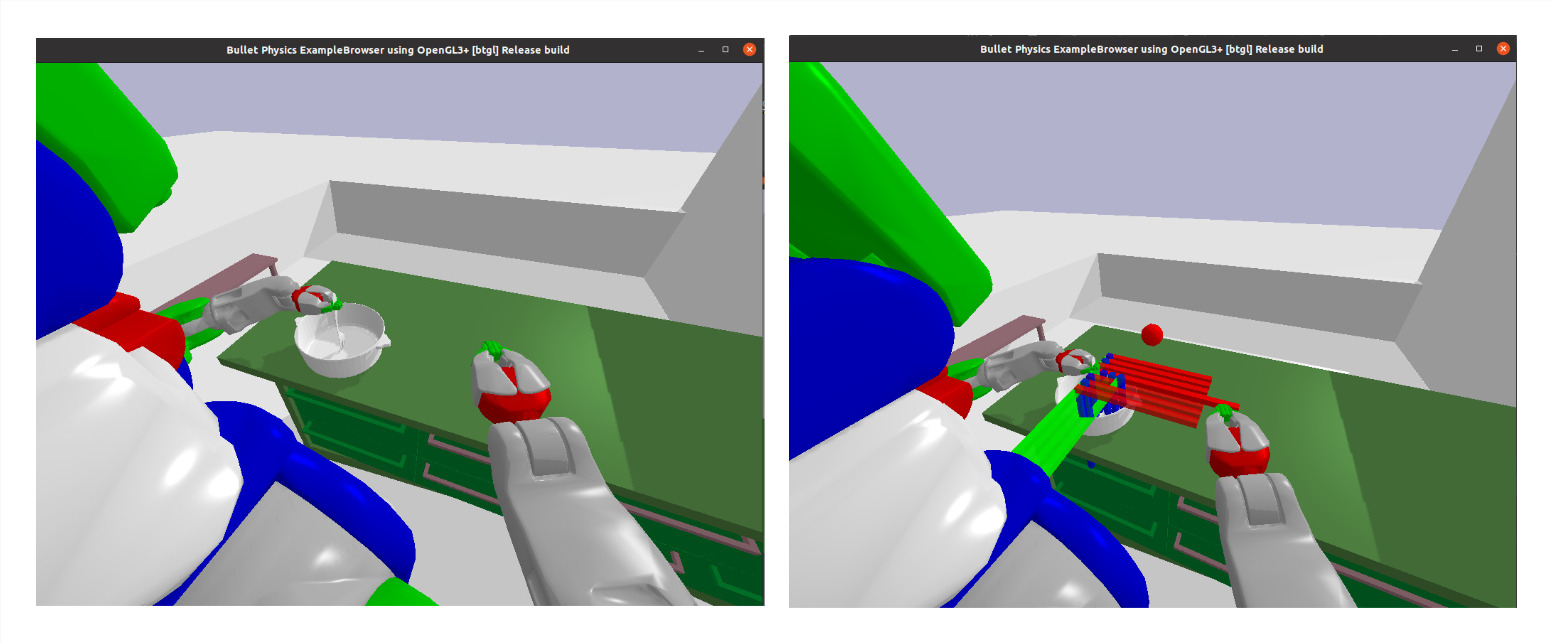
\includegraphics[scale=0.25]{Graphics/folding_evaluation.jpg}
  \caption{Inferred \textit{Folding} Motions}
  \label{fig:mixingverb WikiHow}
\end{figure}

\begin{itemize}
\item Inferred Parameters for \textbf{1-6}: 
 \begin{lstlisting}
  => radius_lower_bound_relative = 0.0, 
  radius_upper_bound_relative = 0.7,
  folding_rotation_shift = 90, 
  repetitive_folding_rotation_shift = 22.5,
\end{lstlisting}
\end{itemize}

\chapter{Knowledge Graph Visualization Tool}
During the process of working on the master's thesis, we were searching for a framework that could visually represent our implemented knowledge graph. Our aim was to clarify the connections and relationships between individual classes. In our search, we found several interesting frameworks that seemed suitable for our needs, which are also mentioned in the \nameref{chap:Related_work} chapter.

However, these solutions weren't entirely satisfactory for us because they lacked some features that we deemed important. Therefore, we decided to develop our own framwework, which should serve as a good visualization framework for our and similar use cases.

In this chapter, we present the framework we developed, from the initial idea to the implementation and the functionalities of our tool.

\section{Main concept}
\label{sec:MainConceps}

We decided on 3 main components that the new framework should include:
\begin{itemize}
    \item Clear Visualization: Our first goal was to facilitate navigation through the knowledge graph by highlighting the relations and classes of the graph as clearly as possible. This could be achieved, for example, by using different colors for different classes or by highlighting a class and its associated classes to which a relation exists. Additionally, we aim to make the graph as clear as possible and reduce the number of nodes to those that are ultimately essential for visualization.
    \item To clarify the relations between the queries, we implement a query builder that, given a class, can point to other classes through the relation, which in turn can point to further classes through another relation, as long as the user desires or there are no further relations. This should be done without having to use the SPARQL query language, making it much easier for the user. The Query Builder outputs a filtered graph with the selected triples.
    \item Inference Query: Since a part of our work relies on inferences, we want to implement an inference query that can indicate inferred parameters based on the input of certain classes. This use case is quite specific to our scenario, but it should also be able to map to other ontologies. The output should be an action tree with the inferred parameters and a visualized graph with the associated classes that play a role in the inference.
\end{itemize}

\section{Architecture}
\label{sec:Architecture}

The architecture consists of a full-stack framework, utilizing \textit{flask} as the web framework in the backend and \textit{HTML} and \textit{JavaScript} for the frontend. 
We use a modified version of \textit{bootstrap} for styling the \textit{HTML}-pages. Additionally, in the backend, we utilize the \textit{rdfLib}(section not yet written, 
\ref{sec:Libraries}) library to process data from the knowledge base. The \textit{JavaScript} functions are responsible for visualizing the graph, which is done using the \textit{vis.js}(section not yet written, 
\ref{sec:Libraries}) library. The following graphics are intended to visually represent a simple description of the architecture, as well as display the folder structure.
\begin{figure}[H]
    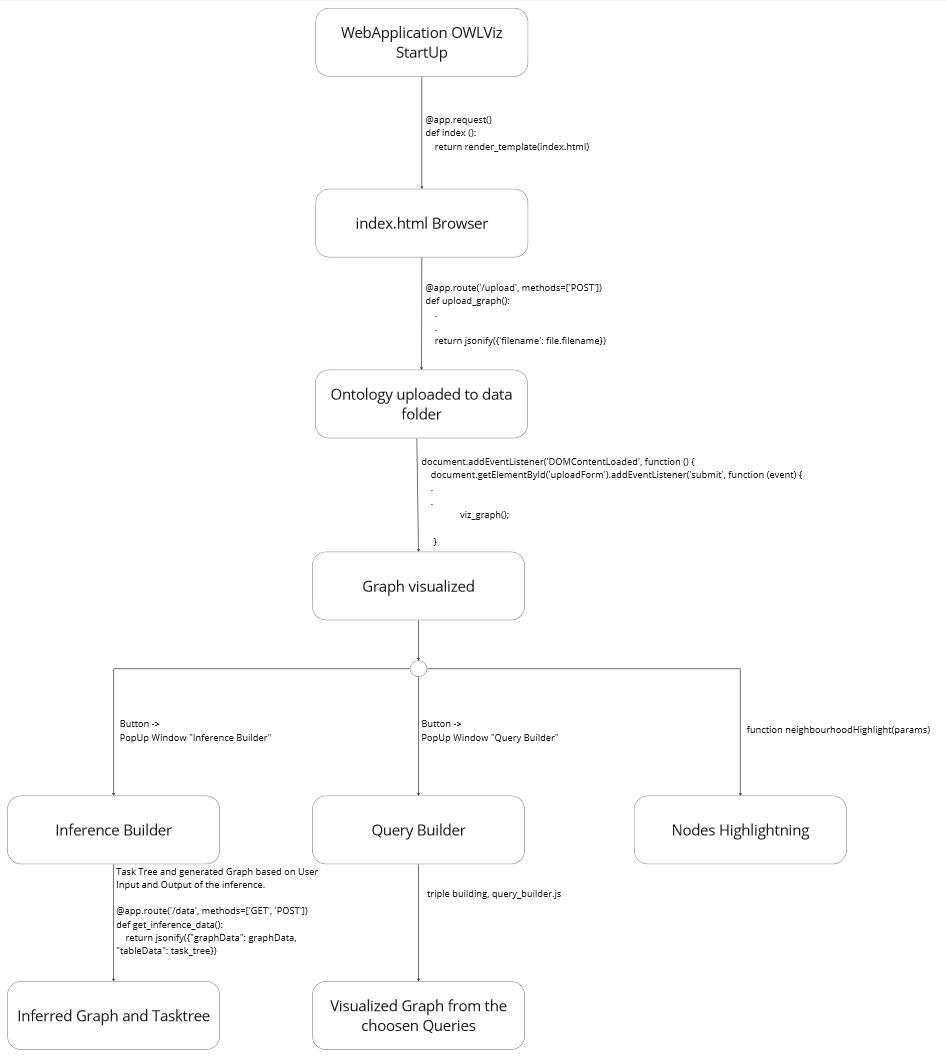
\includegraphics[scale=0.35]{Graphics/OWLViz_architecture.jpg}
    \label{fig:OWLViz_architecture}
    \caption{Architecture chart for the OWLVisualizer framework}
\end{figure}

\dirtree{%
.1 main.py.
.1 templates.
.2 index.html.
.1 data.
.1 static.
.2 graphviz.js.
.2 query\_builder.js.
.1 src.
.2 graph.
.3 graph.py.
.3 coloring.py.
.3 graph\_utility.py.
.2 inference\_builder.py.
.2 query\_builder.py.
}
Below, we want to take a closer look at the individual points of the architecture from a top-level perspective.

\subsubsection{WebApp StartUp} 

To start the application, the Python script \textit{main.py} has to be executed. This can be done using the following command, provided that the necessary libraries have been installed:
\textit{\$: python main.py}

This will start the \textit{flask} web application and open the homepage \textit{index.html}.
\begin{figure}[!ht]
    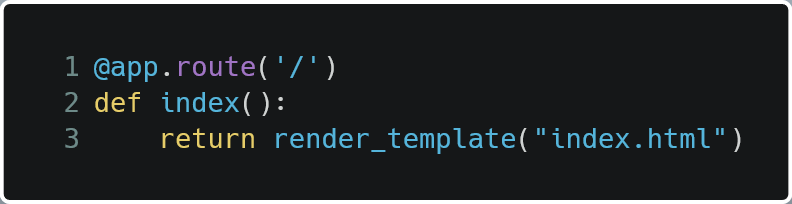
\includegraphics[scale=0.35]{Graphics/def_index.png}
    \caption{\textit{index()} - function.}
\end{figure}

\begin{itemize}
        \item \textit{@app.route("/")} indicates which function is executed first when the framework is started.
        \item \textit{render\_template("index.html")} indicates which \textit{HTML} page is being called, in this case, \textit{index.html}.
\end{itemize}

\subsubsection{Upload Ontology}

The web app initially starts with a (almost) blank \textit{HTML} page, which only contains a navigation bar. 
\begin{figure}[H]
    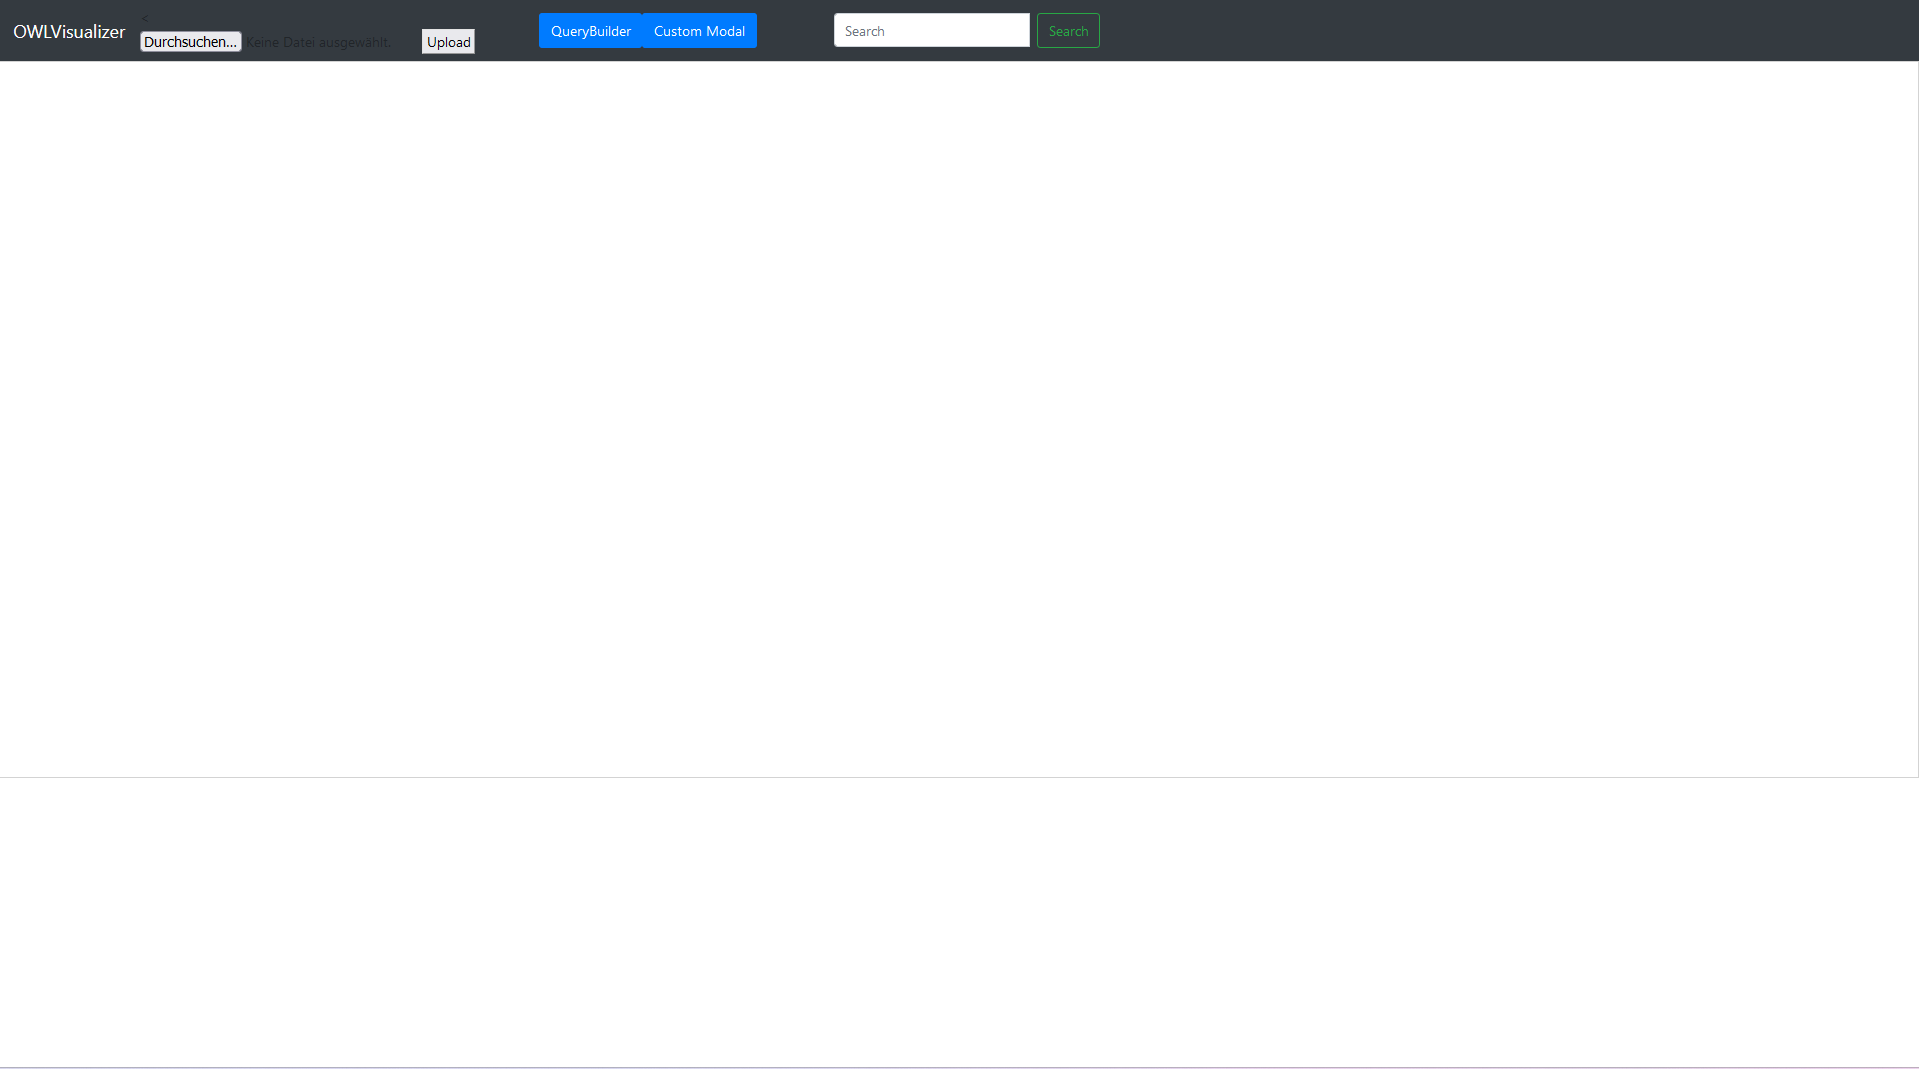
\includegraphics[scale=0.3]{Graphics/webapp_startupt_html.png}
    \caption{Startpage of the framework}
\end{figure}

Now, the user has the option to upload an ontology to work with. The function \textit{upload\_graph()} saves the ontology in the \textit{data} folder.

\begin{figure}[H]
    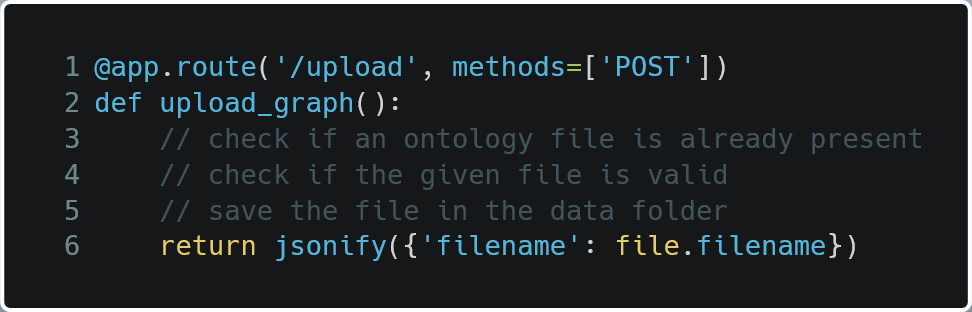
\includegraphics[scale=0.2]{Graphics/upload_graph.png}
    \caption{\textit{upload\_graph()} - function.}
\end{figure}

\subsubsection{Visualized Graph}
Once the ontology has been uploaded, the \textit{JavaScript} function \textit{viz\_graph()} is executed, 
which ultimately visualizes the graph. This function fetches the required sets of nodes and edges from the backend function \textit{get\_graph\_data()}.

\begin{figure}[H]
    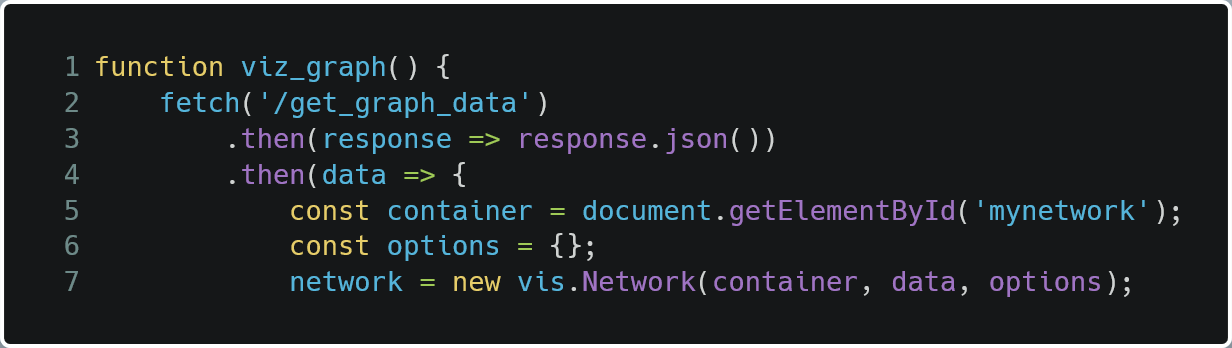
\includegraphics[scale=0.2]{Graphics/viz_graph_function().png}
    \caption{\textit{viz\_graph()} - function.}

\end{figure}

\begin{figure}[H]
    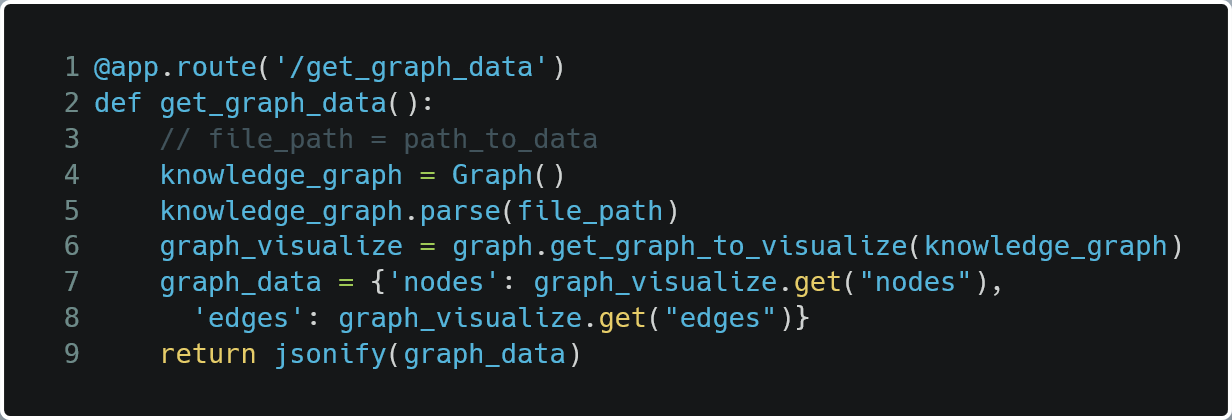
\includegraphics[scale=0.2]{Graphics/get_graph_data.png}
    \caption{\textit{get\_graph\_data()} - function.}

\end{figure}

The data processing is complex and will be further elaborated in the \nameref{sec:Implementation} section. 
Additionally, we have written a section intended to provide a simple introduction to our framework, which can be found in the section 
\nameref{sec:Introducing the framework with a trivial example} . This section aims to illustrate the functionality through a trivial example.
\subsubsection*{Nodes Highlightning}

For large graphs, it can become difficult to maintain an overview of the nodes and their associated relations. 
Therefore, we are implementing a function that highlights a node as well as its neighboring nodes. 
This is intended to make it easier to understand the relationships between a class and its associated nodes. 

The required function is a \textit{JavaScript} function that takes a clicked node as a parameter and calculates its neighboring nodes based on that. 
Subsequently, all nodes are grayed out, and the selected node and its neighbors are restored to their original color. This makes the selected nodes appear "highlighted".

\begin{figure}[H]
    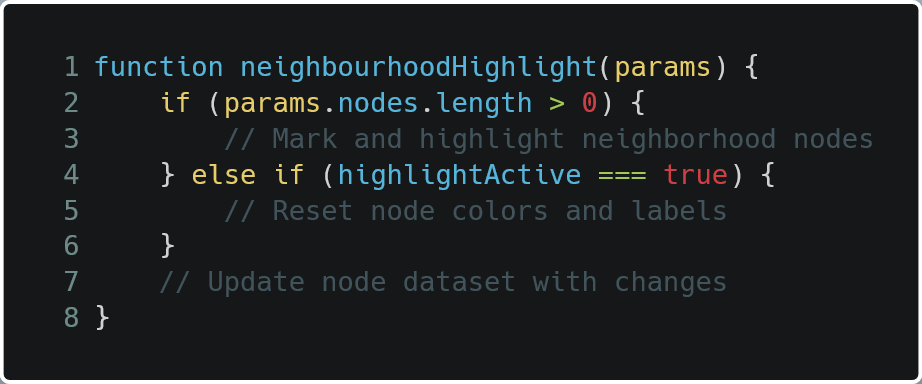
\includegraphics[scale=0.25]{Graphics/neighbourhood_highlighting.png}
    \caption{\textit{neighbourhoodHighlight()}-function}
\end{figure}

Here is an example of a graph with highlighted nodes:

\begin{figure}[H]
    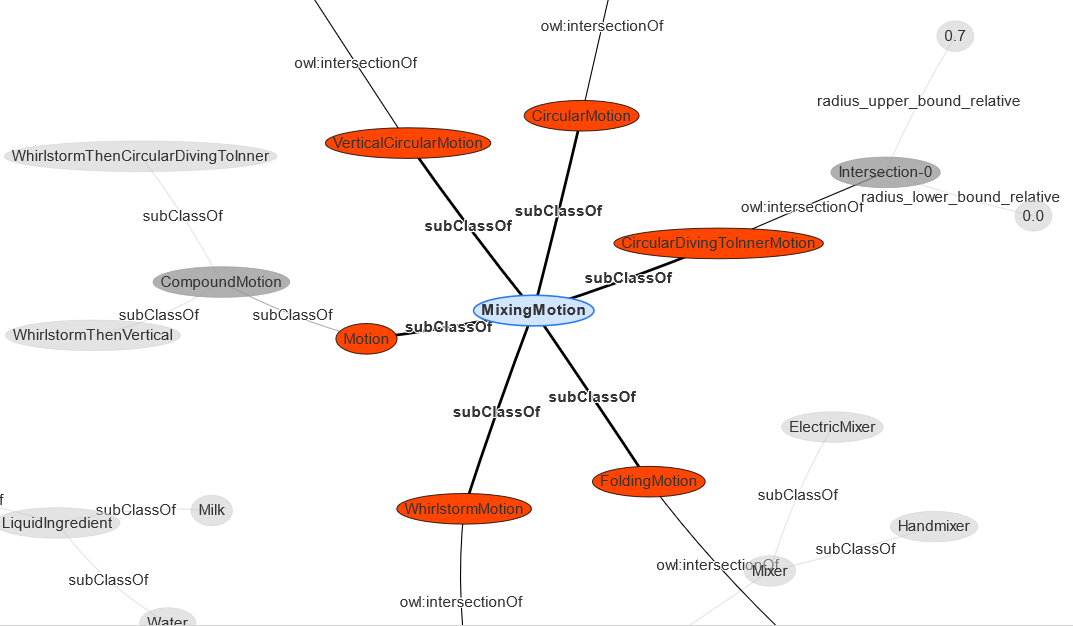
\includegraphics[scale=0.3]{Graphics/nodes_highlight_html.png}
    \caption{graph with highlighted nodes}
\end{figure}

\subsubsection{Query Builder - Naser}
The \textit{QueryBuilder} is another feature of the OWLVisualizer. Its core feature is making triple matching possible without possesing knowledge of  
constructing SPARQL queries. Next to triple matching, visualizing selected triples is made possible, to further visualize relationships between concepts and restrictions
and instances. 
Class restrictions in particular are easily queried using the QueryBuilder, without knowing how to actually query them. 

Another functionality is to construct a SPARQL query from the matched triples for further usage of the user. 

In this section the requirements for this feature are explained.

\paragraph{Requirements}

The \textit{QueryBuilder} needs a processable graph to apply the pattern matching on. 
Two different sources of data can be considered. The parsed graph from rdflib or the graph model for visualization.
Choosing the graph model for visualization is rational since we introduce consistency between graph visualization and
triple matching in the \textit{QueryBuilder}. The main drawback of choosing the graph visualization model is, constructing a
SPARQL query from this model instead of the rdflib parsed graph is made difficult since the graph has to be detransformed into the rdflib parsed graph, to then construct the 
SPARQL query. How this is handled will be discussed in a seperate paragraph. 


\paragraph{Triple Matching}
The concept of triple matching for the \textit{QueryBuilder} is rather simple.
Consider a triple consisting of subject, predicate and object.
A subject is connected via a set of predicates to a set of objects. 
For example we have a subject \textit{A} which has predicates ${\textit{subClassOf}, \textit{equivalentClass}}$
available objects are ${\textit{B}, \textit{C}, \textit{D}}$, where A is a subClassOf B and A is equivalent to C and D. 
Suppose A is picked, then available predicates are ${\textit{subClassOf}, \textit{equivalentClass}}$.
If \textit{subClassOf} is chosen available objects are \textit{B}.
In essence the QueryBuilder is doing exactly that.



\paragraph{Initial Triple Matching}
There is no complete triple matching available if no triples have been selected yet. For example class restrictions are not queryable, they will be queryable once a class
with restrictions has been selected. Initial triple matching is applied to OWL-Classes and instances.

\paragraph{Base Triple Matching} 
Once a triple has been selected more options are available. 
If a OWL-Class has been chosen, the following triples become available:
Relationships with classes connected with subClassOf or equivalentClass.
Classes with class restriction. 
Classes and their instances. 

If an instance has been picked, relationships between other instances are available
between attributes and to which class this instance belongs is available too.

\paragraph{Graphfiltering}
Based on the matched triples provided by the user, the model for graph visualization filtered based upon 
the matched triples to visualize it. The filtered graph contains all information used in the graph visualization in 
the web app to ensure that the view or partial view remains consistent with the original graph.

\paragraph{SPARQL}
To generate a SPARQL query based on the selected triples, triples containing restrictions have to be transformed back into 
rdf graph containing blank nodes. This is relevant for querying in SPARQL, since matching against blanknodes is mandatory to retrieve 
properties and values/classes out of a restriction. 

The resulting query consists off all added triples by the user, where subject, predicate and object is replaced by the 
chosen values. An exception is made for blanknodes, since their indentifiers change each time an ontology is parsed into 
a rdf graph using rdflib. Precise identification is not possible, thus blanknodes have to be replaced with variables, to 
be able to do the triple matching.







\subsubsection{Inference Builder}
The last option for the user to execute functions on a graph is the Inference Builder. 
It's important to note that the Inference Builder is not a generic use case and in this version, it's tailored to the Mixing Graph (see \nameref{chap:Data_representation}). 
In the \nameref{sec:Implementation} section, the implementation is further explained, demonstrating how it could potentially be implemented for other ontologies as well. 
In our case, we infer a motion and its corresponding parameters based on a given task and a potentially long list of ingredients. 
The Inference Builder then generates a graph that only displays the corresponding nodes for clarity, as well as a task tree that can be followed by an agent.
In the first step, the task and the ingredients are sent to the backend for inference, which in turn sends back the inferred motion and parameters to the frontend.

\begin{figure}[H]
    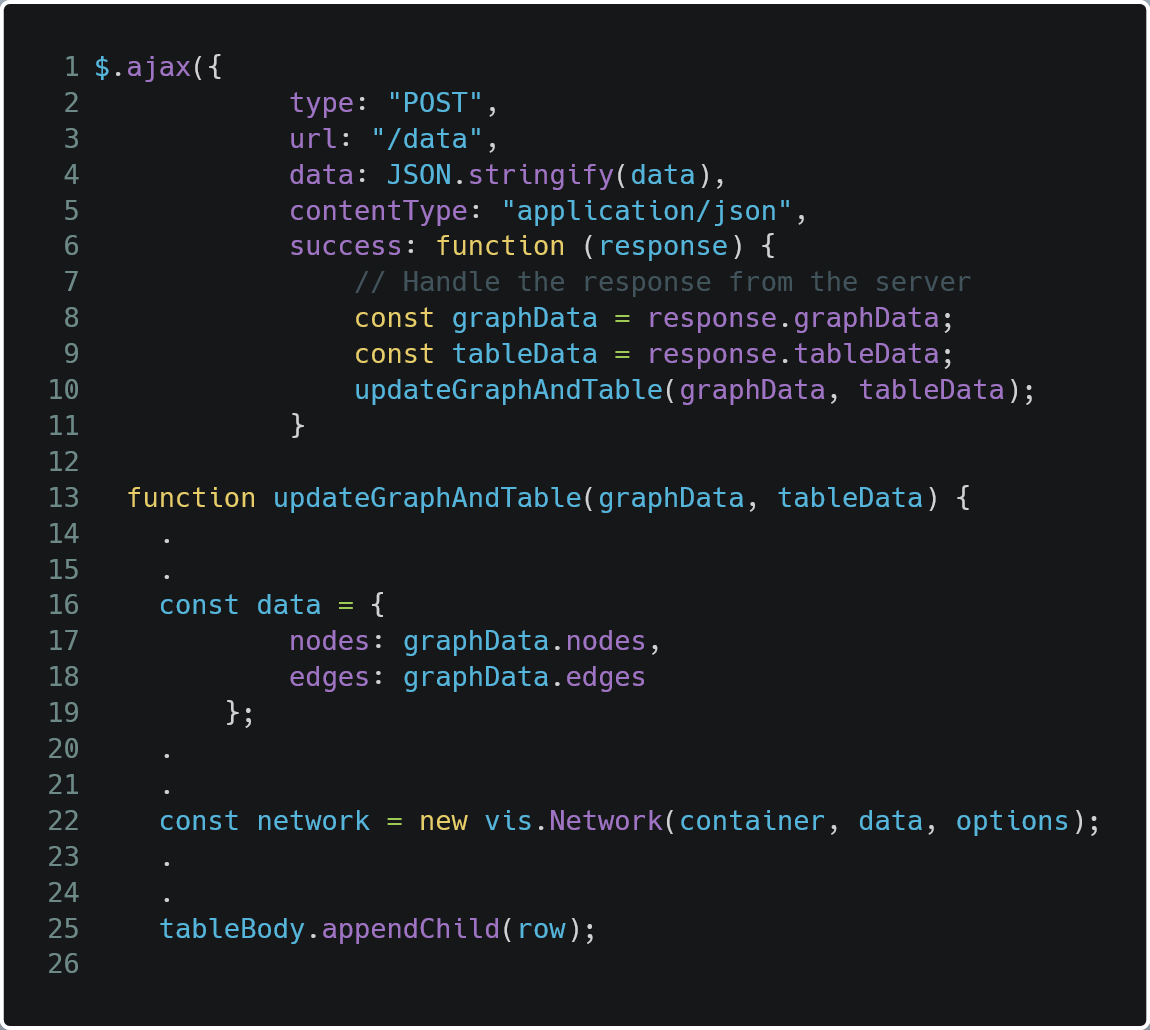
\includegraphics[scale=0.25]{Graphics/inference_builder_js.png}
    \caption{data processing for the inference builder}
\end{figure}

The backend function processes the inference with the received parameters, which are then used for visualization.

\begin{figure}[H]
    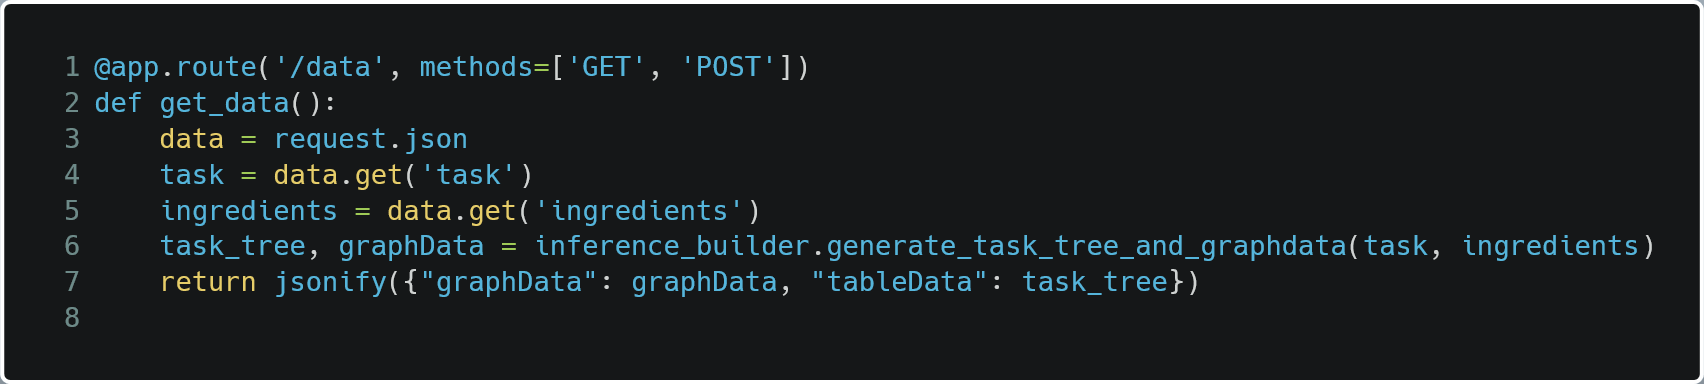
\includegraphics[scale=0.23]{Graphics/get_data.png}
    \caption{\textit{get\_data()}-function}
\end{figure}

After processing the data, the graph and the task tree are visualized based on the user input.

\begin{figure}[H]
    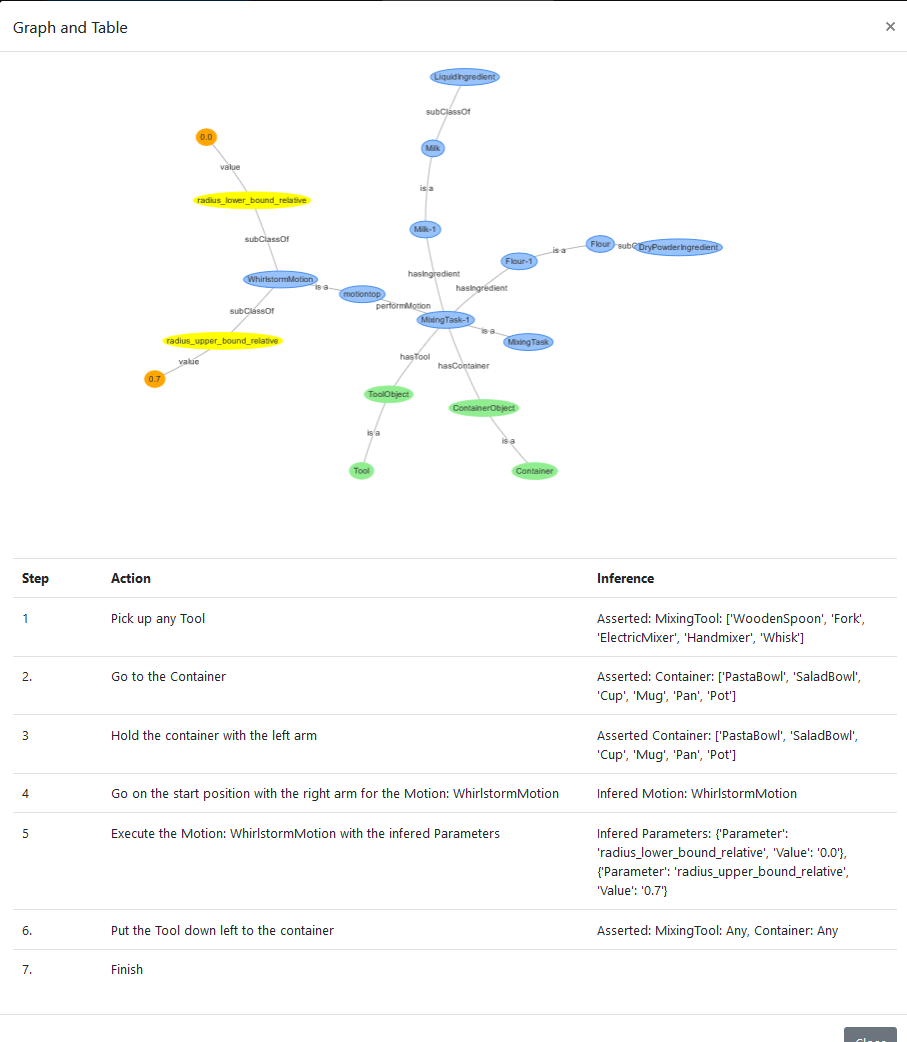
\includegraphics[scale=0.5]{Graphics/new_inference_graph.png}
    \caption{inferred graph and task tree.}
    \label{fig:graph_inferred}
\end{figure}

The data processing and the detailed implementation of the Inference Builder will be further explained in the \nameref{sec:Implementation} section.

\subsubsection{Simple Example of our framework}
\label{sec:Introducing the framework with a trivial example}
In this section, we present a simple example of our framework, from processing the ontology to visualization in the web application. This is intended to facilitate the reader's understanding of our framework. For this purpose, we create a small and simple ontology to explain the program flow in a straightforward manner. Additionally, we aim to demonstrate how this ontology is processed and what the interface between the frontend and backend looks like.

\subsubsection{Simple Ontology}

\begin{figure}[H]
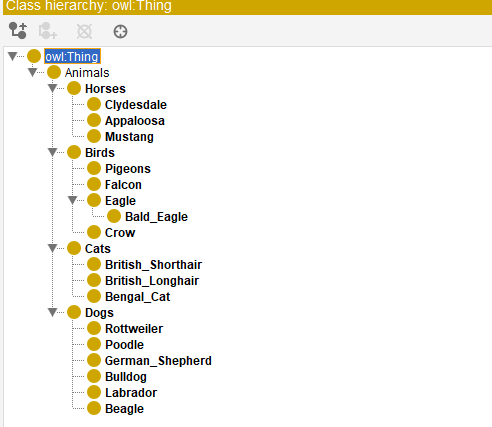
\includegraphics[scale=0.5]{Graphics/simple_ontology_owlviz.png}
\caption{Simple example of an ontology}
\end{figure}

The ontology created for this purpose aims to provide a simple representation of various animal species. It includes superclass categories such as \textit{Horses, Birds, Cats, and Dogs}, as well as subclasses like \textit{Labrador} and \textit{Beagle}, which are subclasses of the \textit{Dog} superclass. This ontology does not depict complicated relations; rather, the individual classes are only connected to each other through the \textit{subClassOf} relation.

\subsubsection{Ontology processing}
Next, the ontology is parsed. Using the \textit{rdfLib}(section not yet written, 
\ref{sec:Libraries}) library , the ontology is read and made queryable. The goal is to retrieve all classes of this ontology along with their associated relations. 
These are then stored in a list, which will be important for visualizing the graph in the frontend.
\begin{figure}[H]
    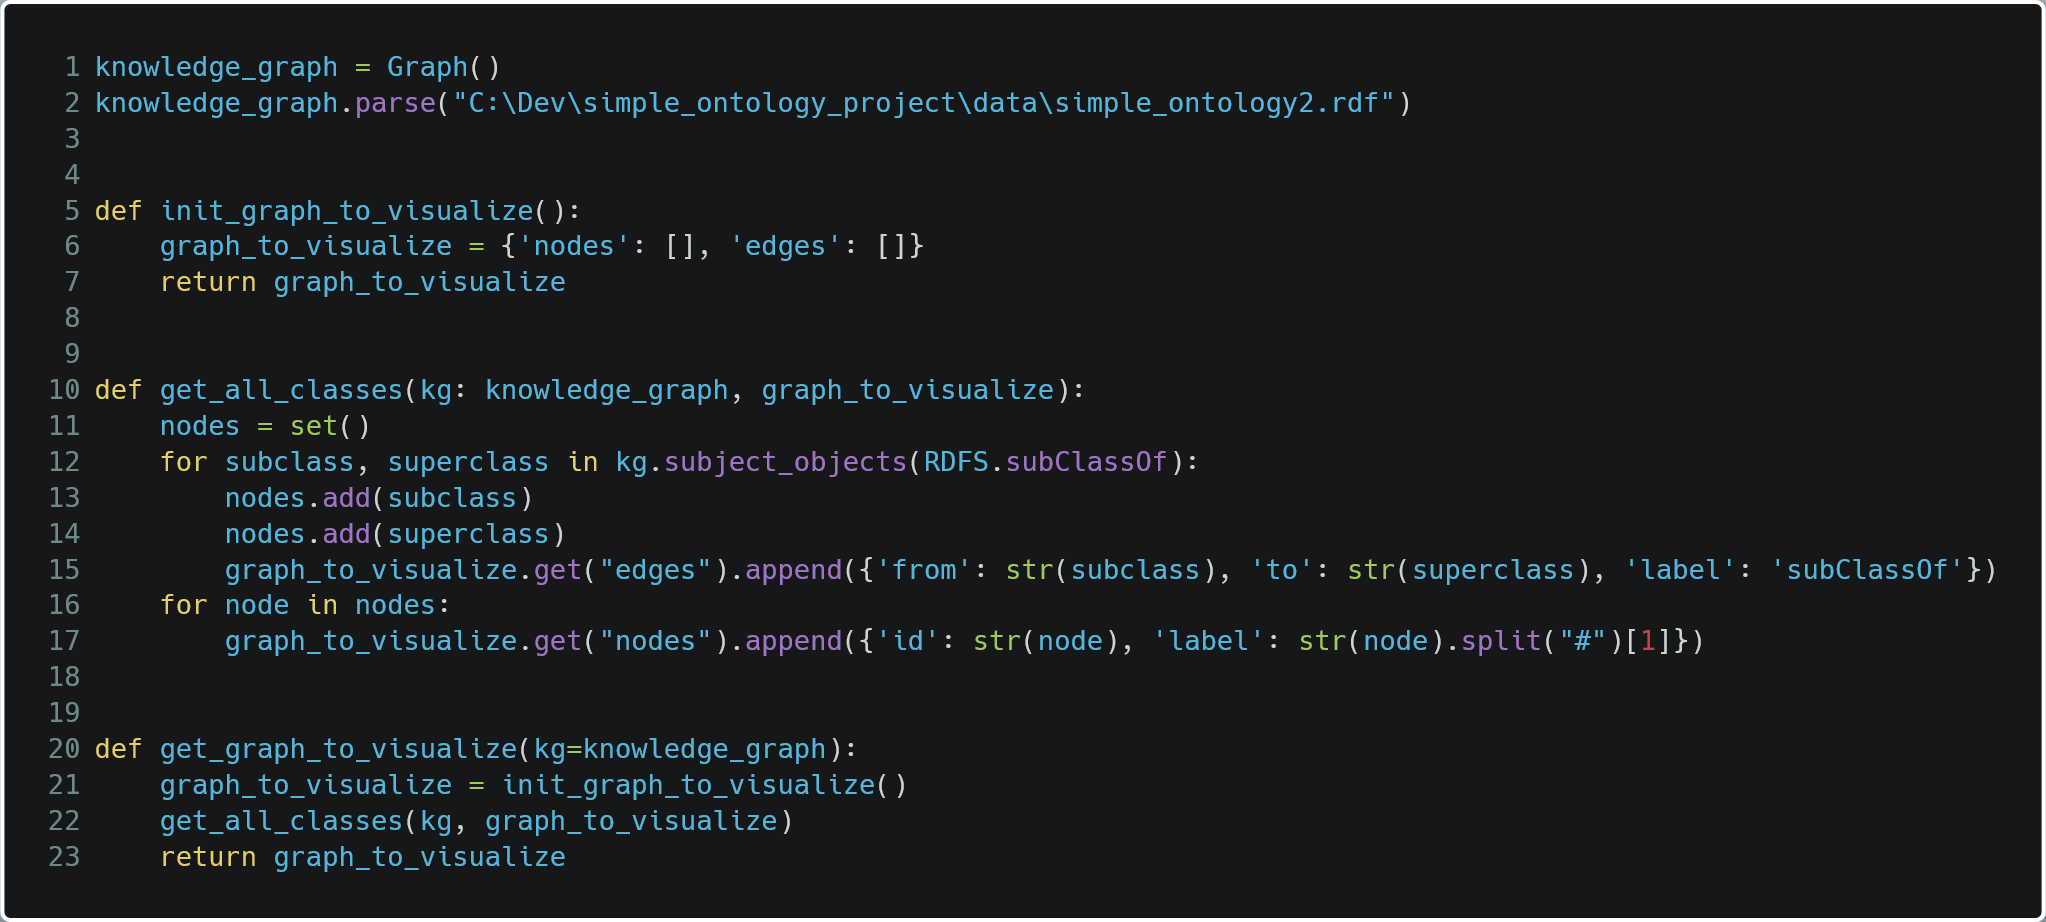
\includegraphics[scale=0.2]{Graphics/simple_ontology_graph_init.png}
    \caption{Graph initialisation}
    \end{figure}
    
\begin{itemize}
    \item Lines 1 and 2: A graph is created, and the ontology is parsed and inserted into this graph.
    \item Lines 5 to 7: This function serves to pass on the set of nodes and edges for the visualization of the graph. The nodes represent the classes, while the edges represent the relations.
    \item Lines 10 to 17: This function searches the graph for all classes, which are distinguished between superclass and subclass. The edges then point from a superclass to its corresponding subclass. Both classes are also added to a list of nodes.
    \item Lines 20 to 23: The set of nodes and edges is initialized for the graph and is now ready for visualization.
\end{itemize}

With that, the processing of the ontology for the set of nodes and edges for visualization has been completed. Now, we want to visualize these sets.

\subsubsection{From Backend to FrontEnd: Visualization}

As a reminder: The framework we are using is \textit{flask}, which facilitates communication between the frontend, consisting of \textit{HTML}, \textit{CSS}, and \textit{JavaScript}, 
and our backend, where the graph is prepared for visualization. First, we'll explain the communication with the frontend.

\begin{figure}[H]
    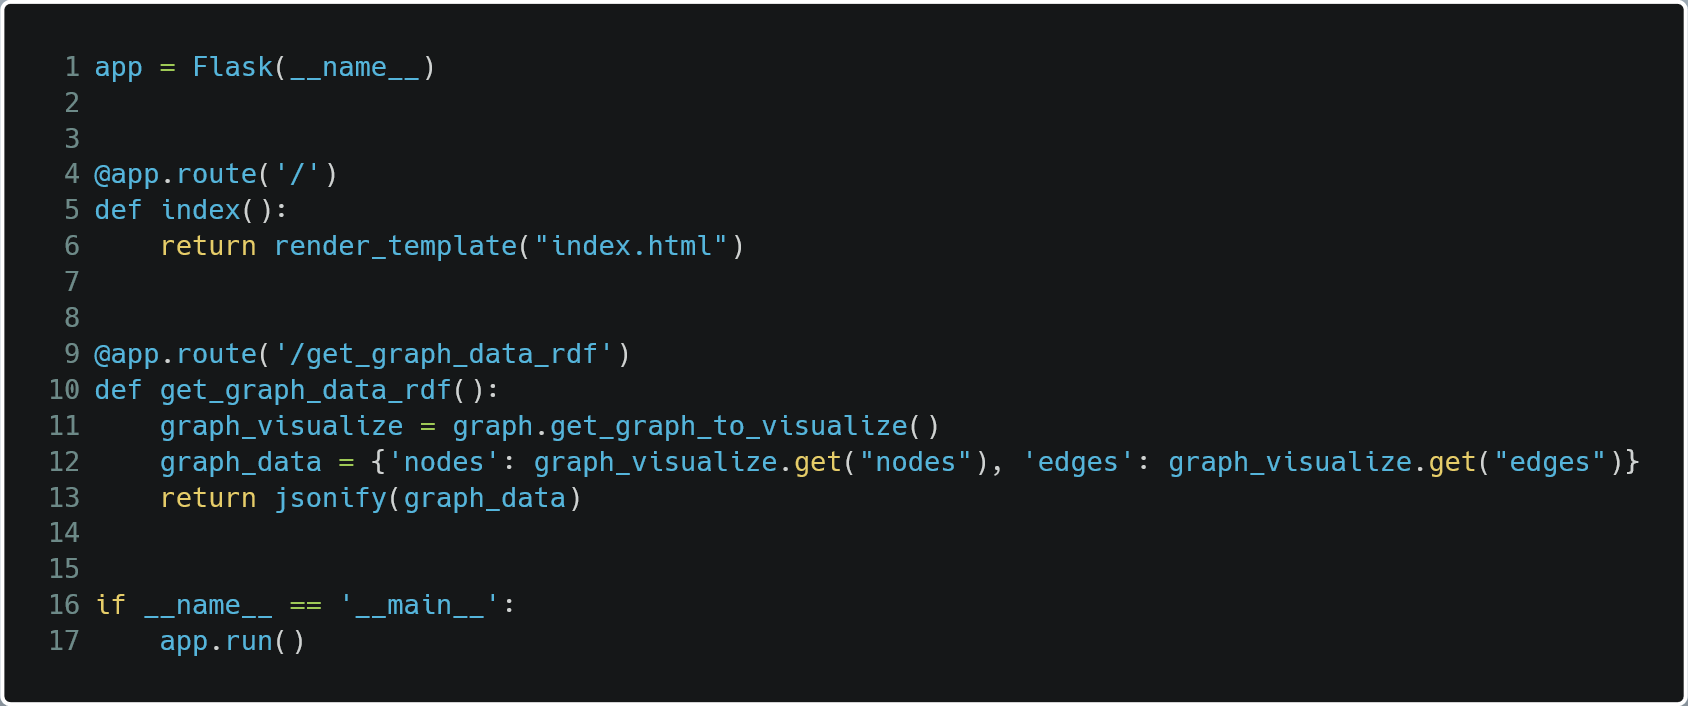
\includegraphics[scale=0.2]{Graphics/simple_ontology_flask.png}
    \caption{Interface between Front and BackEnd}
    \end{figure}
    
\begin{itemize}
    \item Lines 1 to 6: When the application starts, the \textit{HTML} page \textit{index.html} is called.
    \item Lines 9 to 17: When the function \textit{get\_graph\_data\_rdf} is called, the set of nodes and edges is retrieved in a format that can be processed by the \textit{JavaScript} library \textit{vis.js}.
\end{itemize}

The function \textit{get\_graph\_data\_rdf} is called in the frontend \textit{JavaScript}.

\begin{figure}[H]
    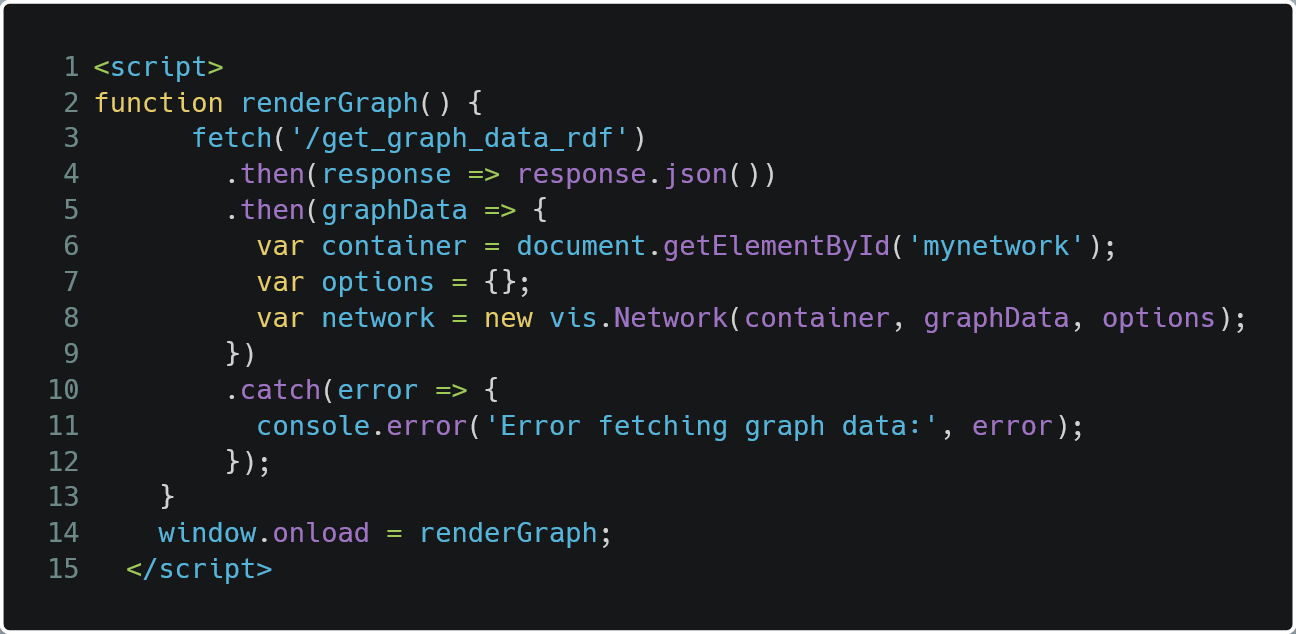
\includegraphics[scale=0.23]{Graphics/simple_ontology_js.png}
    \caption{trivialized example of the FrontEnd}
    \end{figure}

The graph is created using the data extracted from the output of the function 
\textit{get\_graph\_data\_rdf}. In line 14, it is specified that the function for rendering the graph is called directly upon loading the \textit{HTML} page.

\begin{figure}[H]
    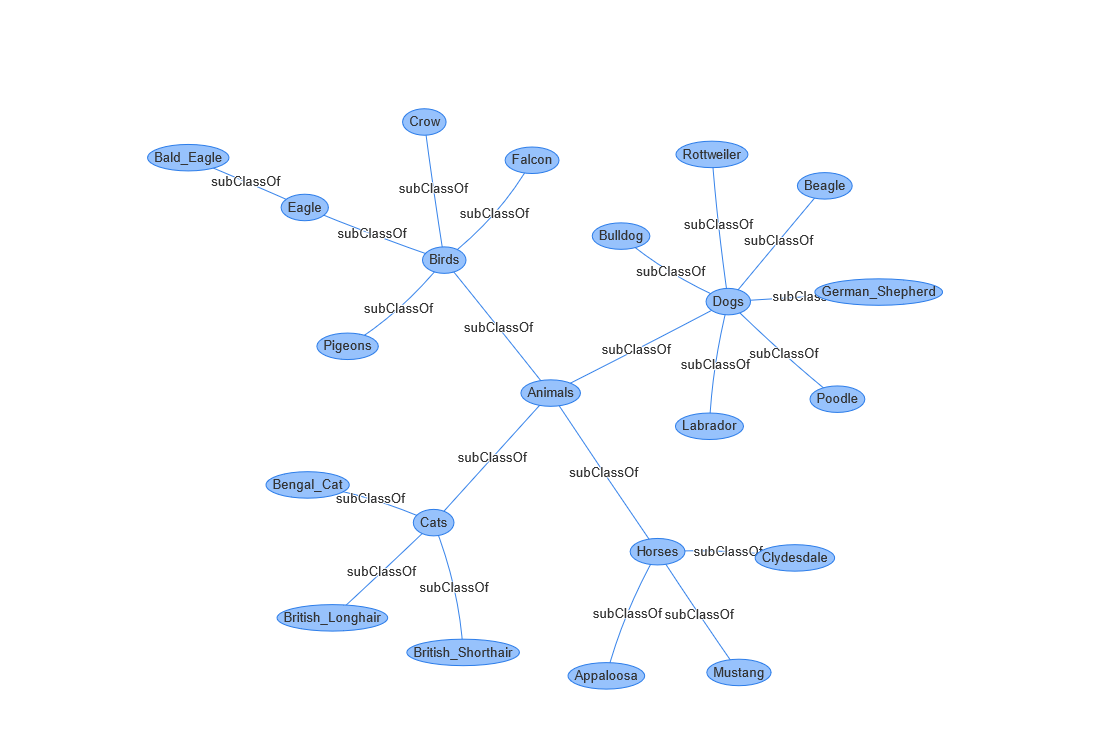
\includegraphics[scale=0.45]{Graphics/simple_graph.png}
    \caption{generatd example-graph}
\end{figure}


This example illustrated the process of visualizing a simple ontology. However, the ontologies we tested during the implementation were much more complex and required various specific implementations to visualize them. Additionally, we made several improvements to the visualization itself compared to the standard graph. The implementation of the backend, as well as the three different functions (see \nameref{sec:MainConceps}), will be described in more detail in the next section.
\section{Implementation}
\label{sec:Implementation}

This section explains the detailed implementation of the framework and highlights the challenges and solutions encountered during implementation. In the previous section, we provided a trivial example intended to serve as an introduction for users to understand the framework's basics. However, since ontologies can vary in structure and some relations can be complex, a simple implementation may not suffice in most cases.

We will begin by explaining the implementation of the backend, and towards the end of the section, we will also address some aspects of the frontend. In the conclusion, we will touch upon points that, in our opinion, could be implemented in the future and discuss any problems/limitations this framework might have.
\subsection{BackEnd}

As explained in the \nameref{sec:Architecture} section and demonstrated in the Introductory Example section (see: \nameref{sec:Introducing the framework with a trivial example}), the framework uses \textit{flask} as its backend interface. 
This ultimately serves to send processed data to the frontend or receive data from it. Now, we'd like to explain how this data is processed and how it has been adequately prepared.
\subsubsection{Graph Verarbeitung - Work in Progress}

To visualize a graph using the JavaScript library \textit{vis.js} (NOTE), we need a set of nodes and edges. An example of how these could be processed was explained here (NOTE). The existing classes of an ontology are not always connected only by the \textit{subClassOf} relation. Some relations pose challenges in the graph because lists of possible classes related to a superclass can also appear. This poses a problem for visualization because in such cases, so-called \textit{Blank Nodes} appear. These nodes do not represent any information but merely serve as connection nodes between 2 or more classes. These nodes are connected by relations such as \textit{owl:intersectionOf}, \textit{owl:first}, or \textit{owl:rest} and have no added value for our visualization. The first challenge was to adequately process these nodes to remove \textit{Blank Nodes} from the visualized graph and to represent the correct relation between the classes between which these \textit{Blank Nodes} existed

\subsubsection{Implementation of the Query Builder - Work in Progress}


\subsubsection{Implementation of the Inference Builder}
As described in the \nameref{sec:Architecture}, the Inference Builder is intended to visualize and organize the results of inference within the ontology. 
The inference refers to defined \textit{SWRL} rules (see: \nameref{sec:SWRL}), which can then be queried using the \textit{OWLReady2} library (see: \nameref{sec:OWLReady}).
Therefore, the implementation assumes this type of rules. The rules implemented by us were explained in the \nameref{chap:Motions} chapter. 
Ultimately, the goal is to execute the inference based on user input and visualize the results.
\paragraph{User Input}

The user selects a task and any number of ingredients.
\begin{figure}[H]
    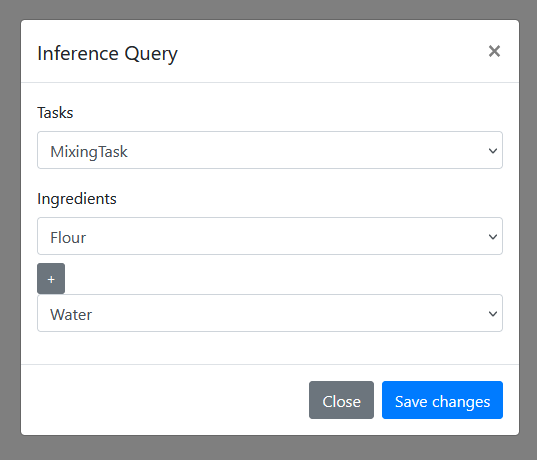
\includegraphics[scale=0.45]{Graphics/inference_user_input.png}
    \caption{Select fields for the inference.}
\end{figure}
These data are extracted from the ontology using the \textit{rdfLib}(section not yet written, 
\ref{sec:Libraries}). The following code will explain this further.

\begin{figure}[H]
    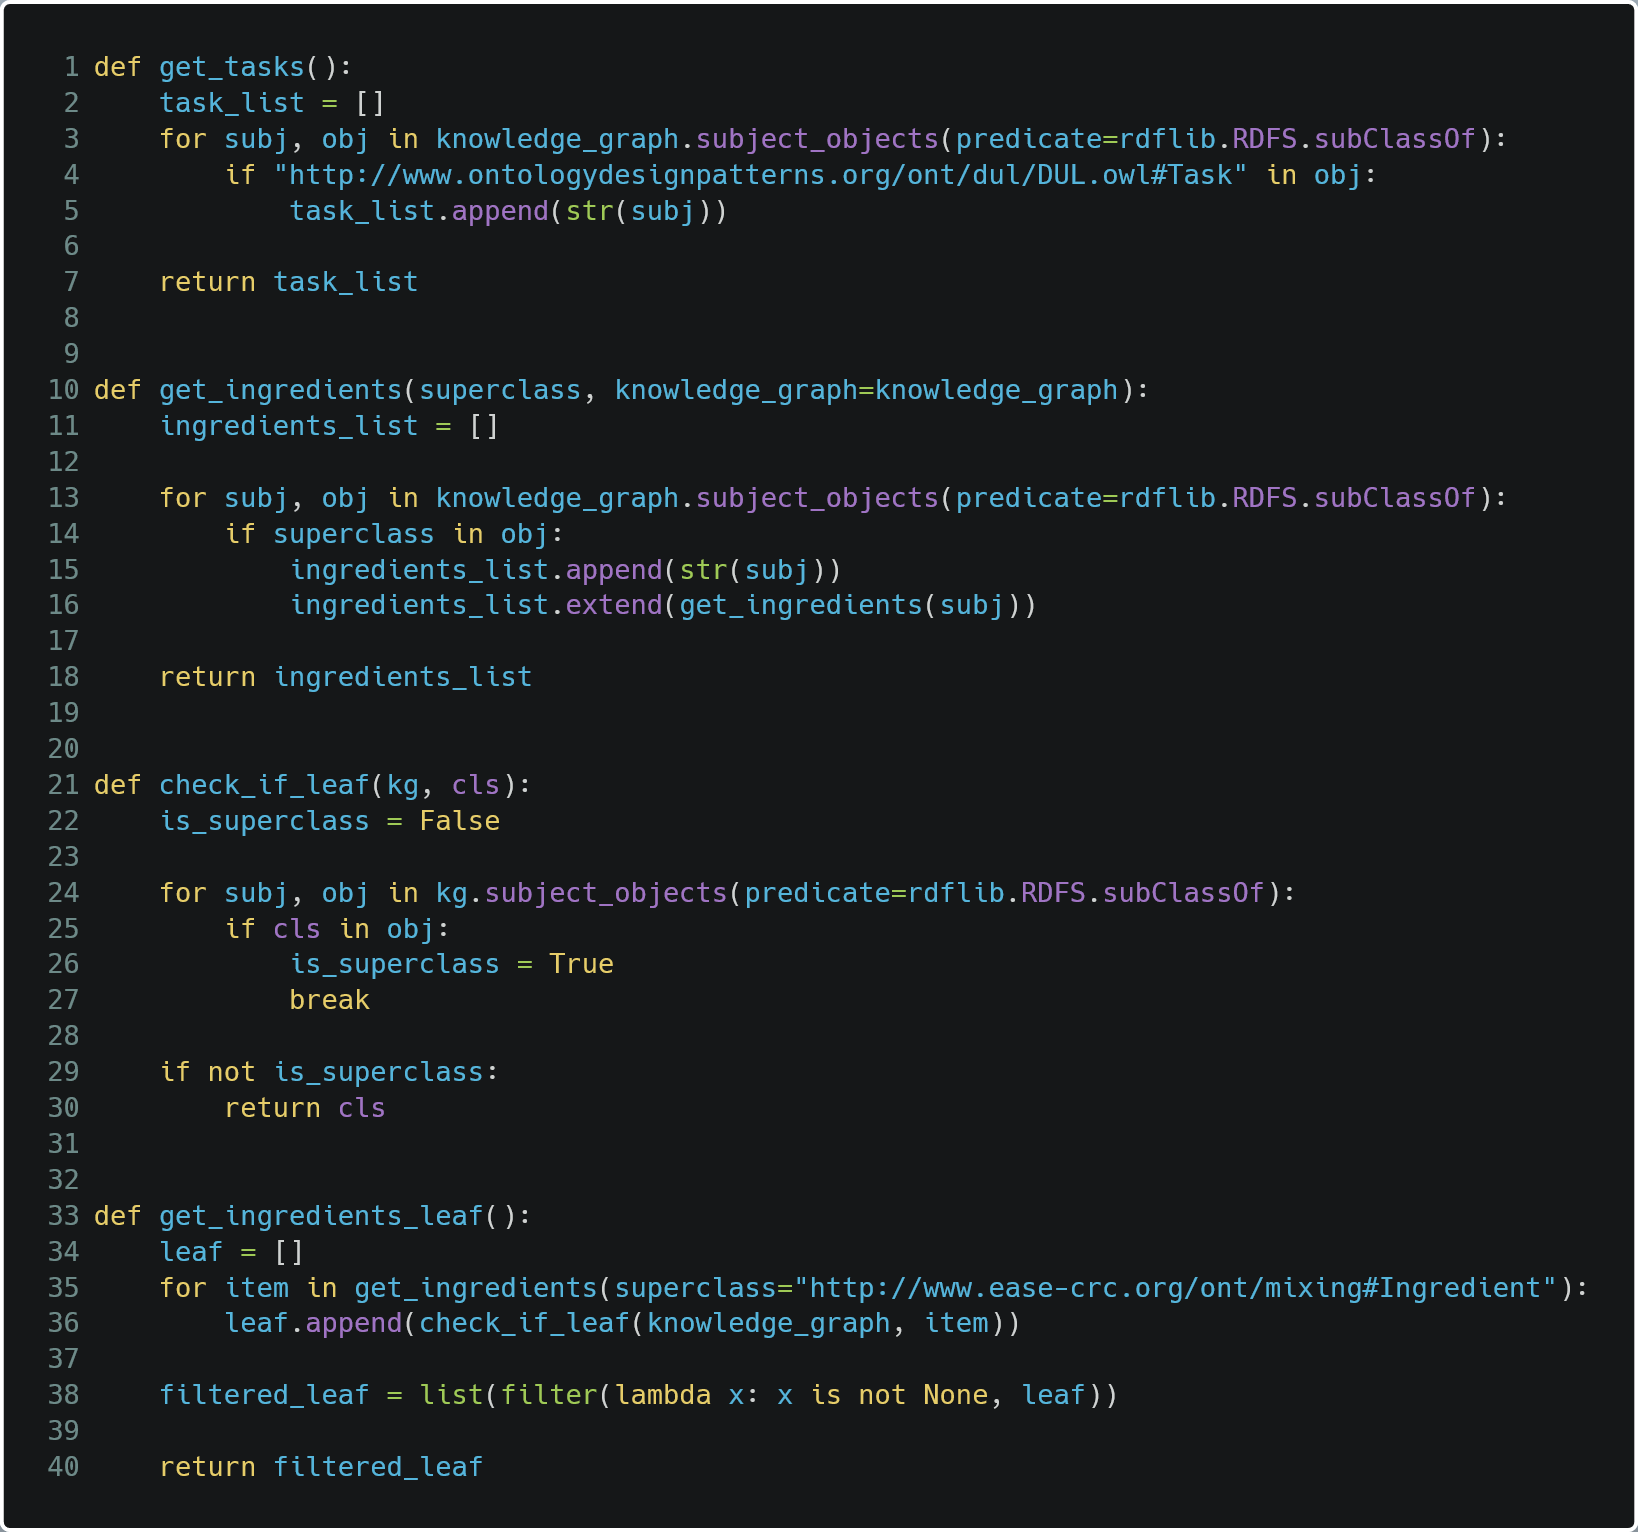
\includegraphics[scale=0.22]{Graphics/get_tasks_ingredients.png}
    \caption{Code snippet for querying the tasks and ingredients from the ontology}
\end{figure}

\begin{itemize}
    \item Lines 1 - 7: Each triple where the predicate of the relation matches \textit{subClassOf} is queried. Additionally, it checks whether the object corresponds to the class \textit{Task}. These elements are then added to a list, which is also returned.
    \item Lines 10 - 18: Similar to the above function, the subclasses of ingredients are returned. The only difference is that the function is called recursively since the class \textit{Ingredients} has subclasses at multiple levels. Therefore, it also checks which class has no more subclasses.
    \item Lines 21 - 30: This function checks whether a given class corresponds to a leaf in a graph, meaning this class itself has no subclasses.
    \item Lines 33 - 40: This function ultimately returns the list of ingredients available for the user's selection.
\end{itemize}

These data are sent to the frontend using the following function:

\begin{figure}[H]
    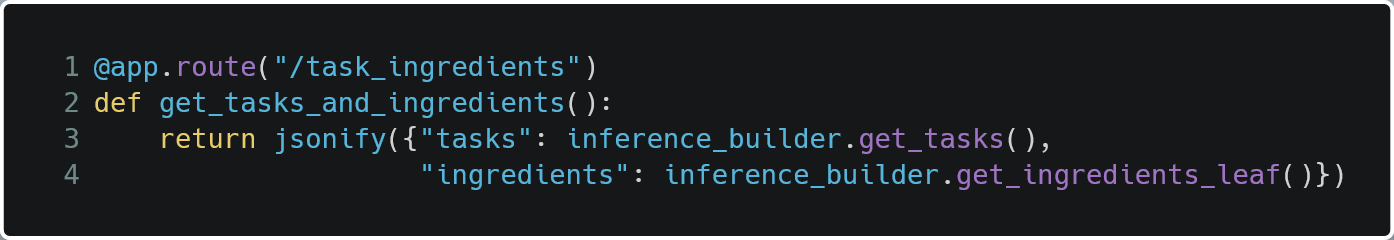
\includegraphics[scale=0.25]{Graphics/inference_main.png}
    \caption{\textit{get\_tasks\_and\_ingredients()}-function}
\end{figure}

The previously described functions are called, and the data is sent to the frontend in \textit{JSON} format. In the frontend, this data is fetched and processed.

\begin{figure}[H]
    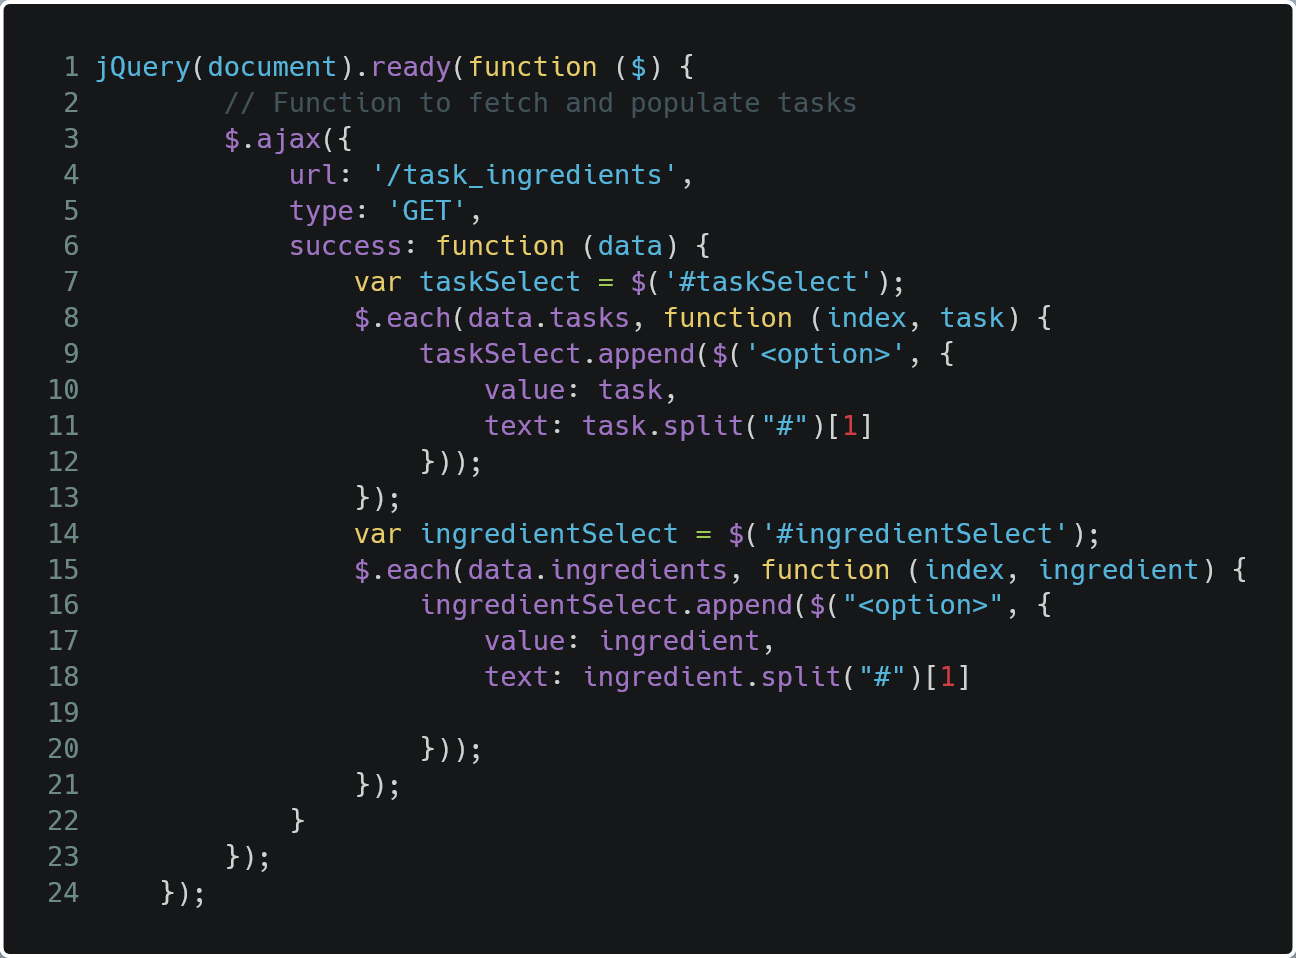
\includegraphics[scale=0.22]{Graphics/inference_frontend_fetch.png}
    \caption{Data is fetched in the FrontEnd}
\end{figure}

This function populates the entries of the select fields for task and ingredient selection with the data from the backend. 
By doing so dynamically, it ensures that even if the ontology has new entries in these classes, they will always be available for the user's selection.

\paragraph{Inference}
\label{par:Inference}

An example can illustrate the process of inference calculation. Taking the above example (see: \ref{fig:graph_inferred}), we have the input task: \textit{MixingTask} and the ingredients: \textit{Flour} and \textit{Water}. 
These two ingredients correspond to the superclasses \textit{DryPowderIngredient} and \textit{LiquidIngredient}, respectively (see: \nameref{chap:Data_representation} for more information 
about the structure of the ontology.). This combination ultimately corresponds to the \nameref{sec:SWRL}-Rule:
\begin{lstlisting}
MixingTask(?x) ^ DryPowderIngredient(?ing1) ^ hasIngredient(?x, ?ing1)
^ LiquidIngredient(?ing2) ^ hasIngredient(?x, ?ing2) ^ Motion(?motion) 
^ performMotion(?x, ?motion) -> WhirlstormMotion(?motion)
\end{lstlisting}

From this, the motion \textit{WhirlstormMotion} is inferred with the corresponding parameters:
\begin{lstlisting}
    radius_lower_bound_relative  0.0
    radius_upper_bound_relative  0.7
\end{lstlisting}
To calculate this inference, we use the library \textit{OWLReady2} (see: \nameref{sec:OWLReady}), which enables us to utilize a reasoner for the inference.
\begin{figure}[H]
    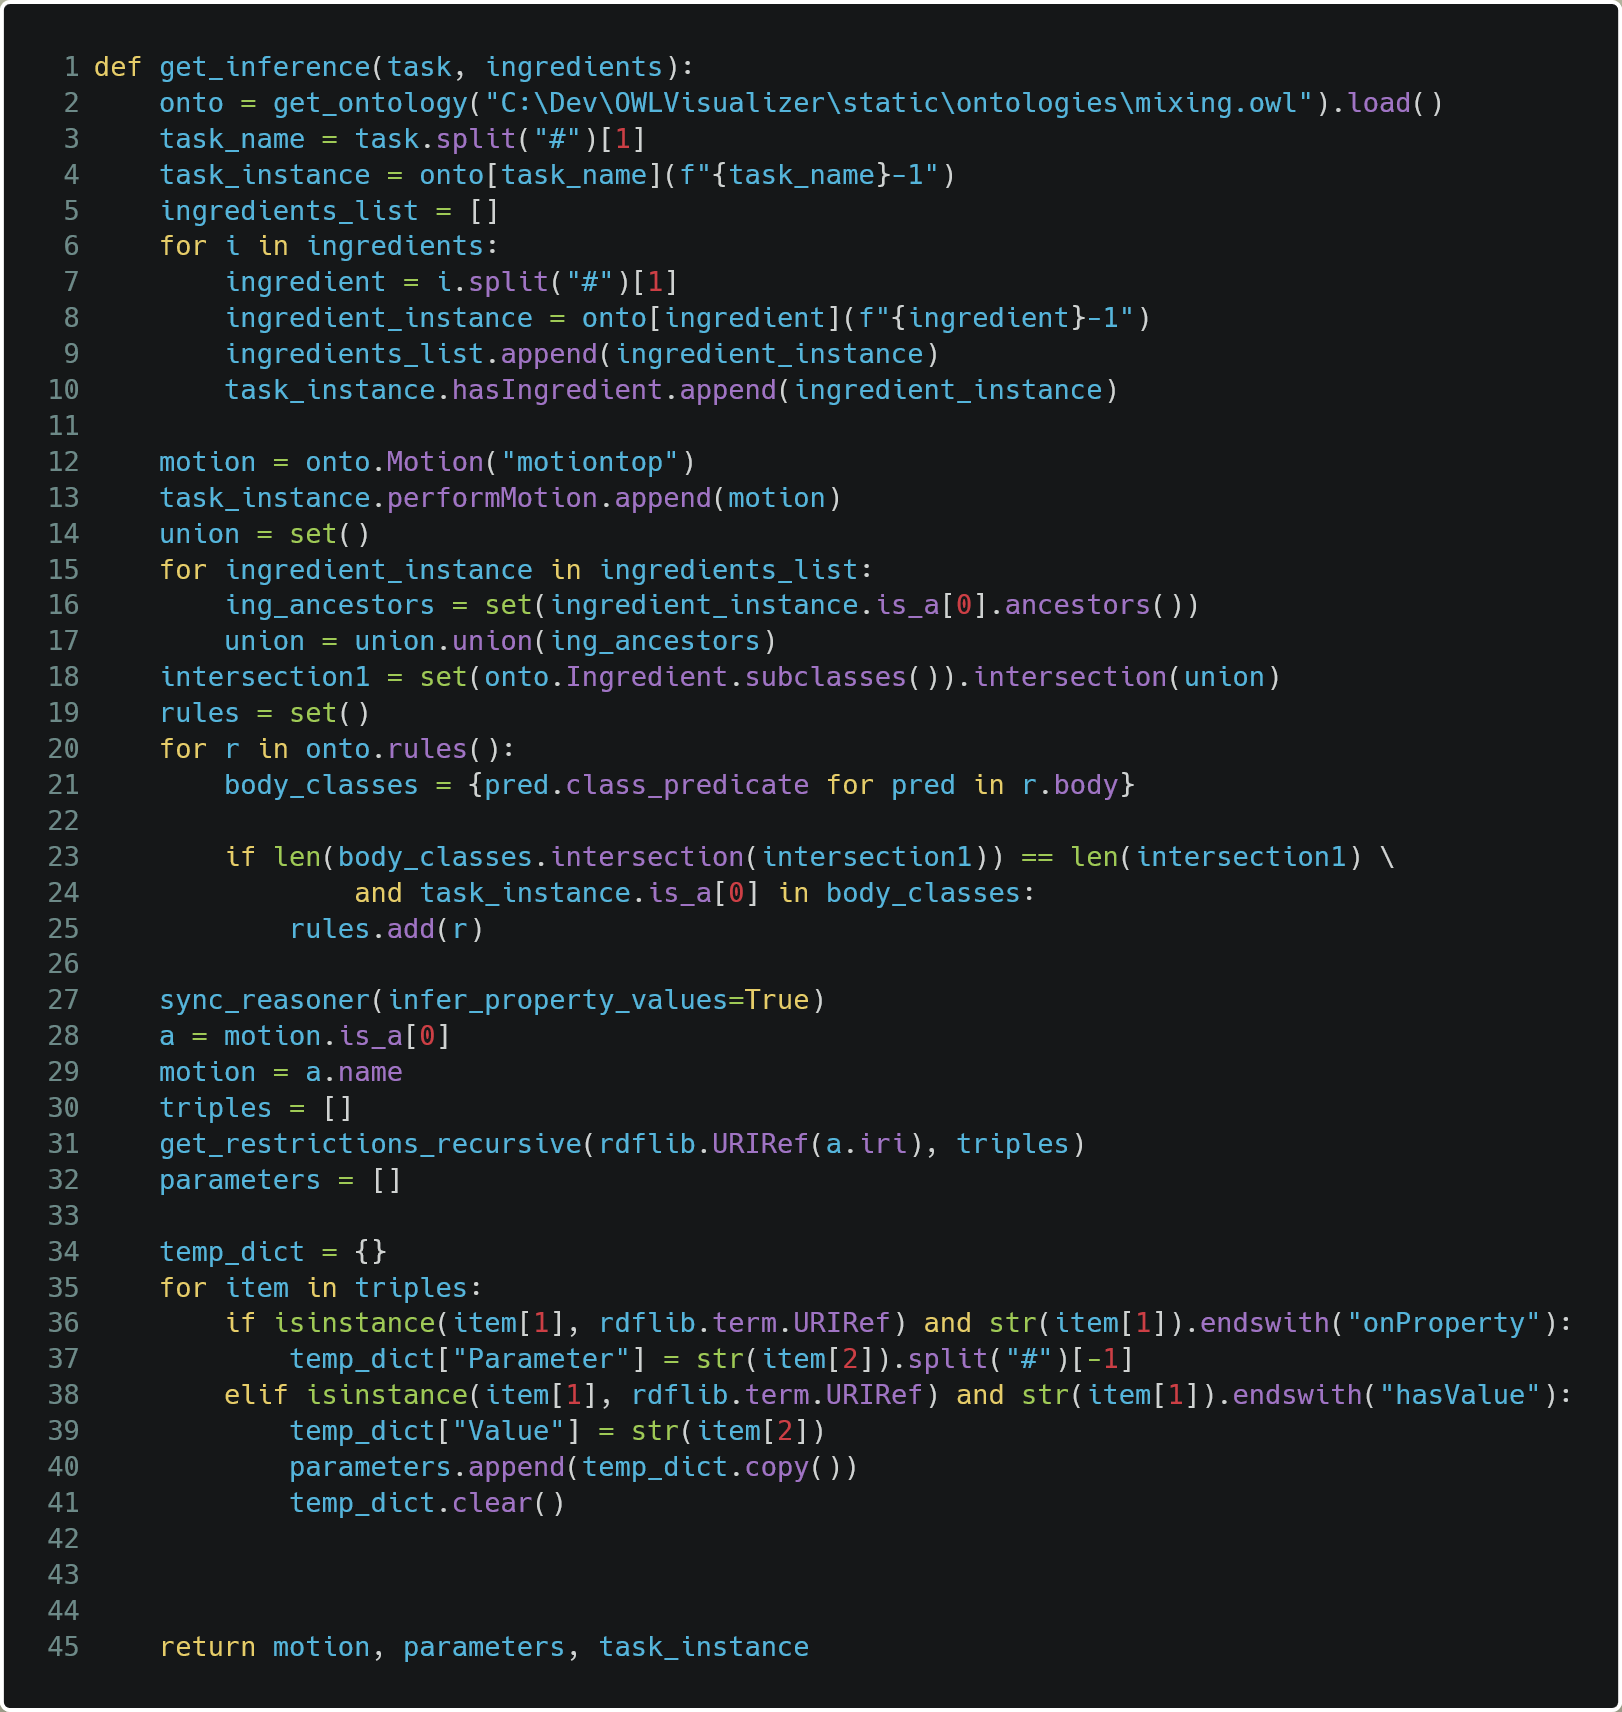
\includegraphics[scale=0.23]{Graphics/get_inference.png}
    \caption{Inference function}
\end{figure}
\begin{itemize}
    \item Lines 1 - 10: The classes are instantiated. The function takes parameters \textit{task}, corresponding to a task, and \textit{ingredients}, corresponding to a list of ingredients. In line 2, the ontology for the \textit{OWLReady2} library is instantiated to utilize the reasoner. In lines 3 and 4, the \textit{task} is instantiated. Since the task comes as input in the full \textit{IRI} format, it needs to be processed first. From lines 5 to 10, the same is done analogously for the ingredients, this time only for a list of ingredients. Subsequently, the instances of the \textit{ingredients} are added to the instance of \textit{task}.
    \item Lines 12 - 13: A top-level \textit{Motion} is instantiated to indicate that the \textit{Motion} is inferred during reasoning. ???
    \item Lines 14 - 18: Since the superclasses of the \textit{ingredients} are important for the rules, they are added to a set which will be used later for inference.
    \item Lines 19 - 25: The existing rules are examined and matched with the input to infer the correct \textit{SWRL} rules.
    \item Lines 27 - 45: Here, the reasoner is first started. The inferred motion is stored, and now it is about determining the required parameters based on the motion. These parameters are then stored in a dictionary. The function returns the motion, the parameters, and the instance of \textit{task}.
\end{itemize}

\paragraph{Preparing the Output}
For clarity, we have decided to reduce the graph to only the classes used in the inference. The middle node of the graph represents the task instance selected by the user. 
From this node, you can reach the other classes that are important for the inference. 
These classes correspond to the classes of the ingredients, i.e., the ingredient instances selected by the user, the inferred motion along with parameters, 
and each instance for the tools and containers, each of which can represent any possible combination if no selection has been made.
\begin{figure}[H]
    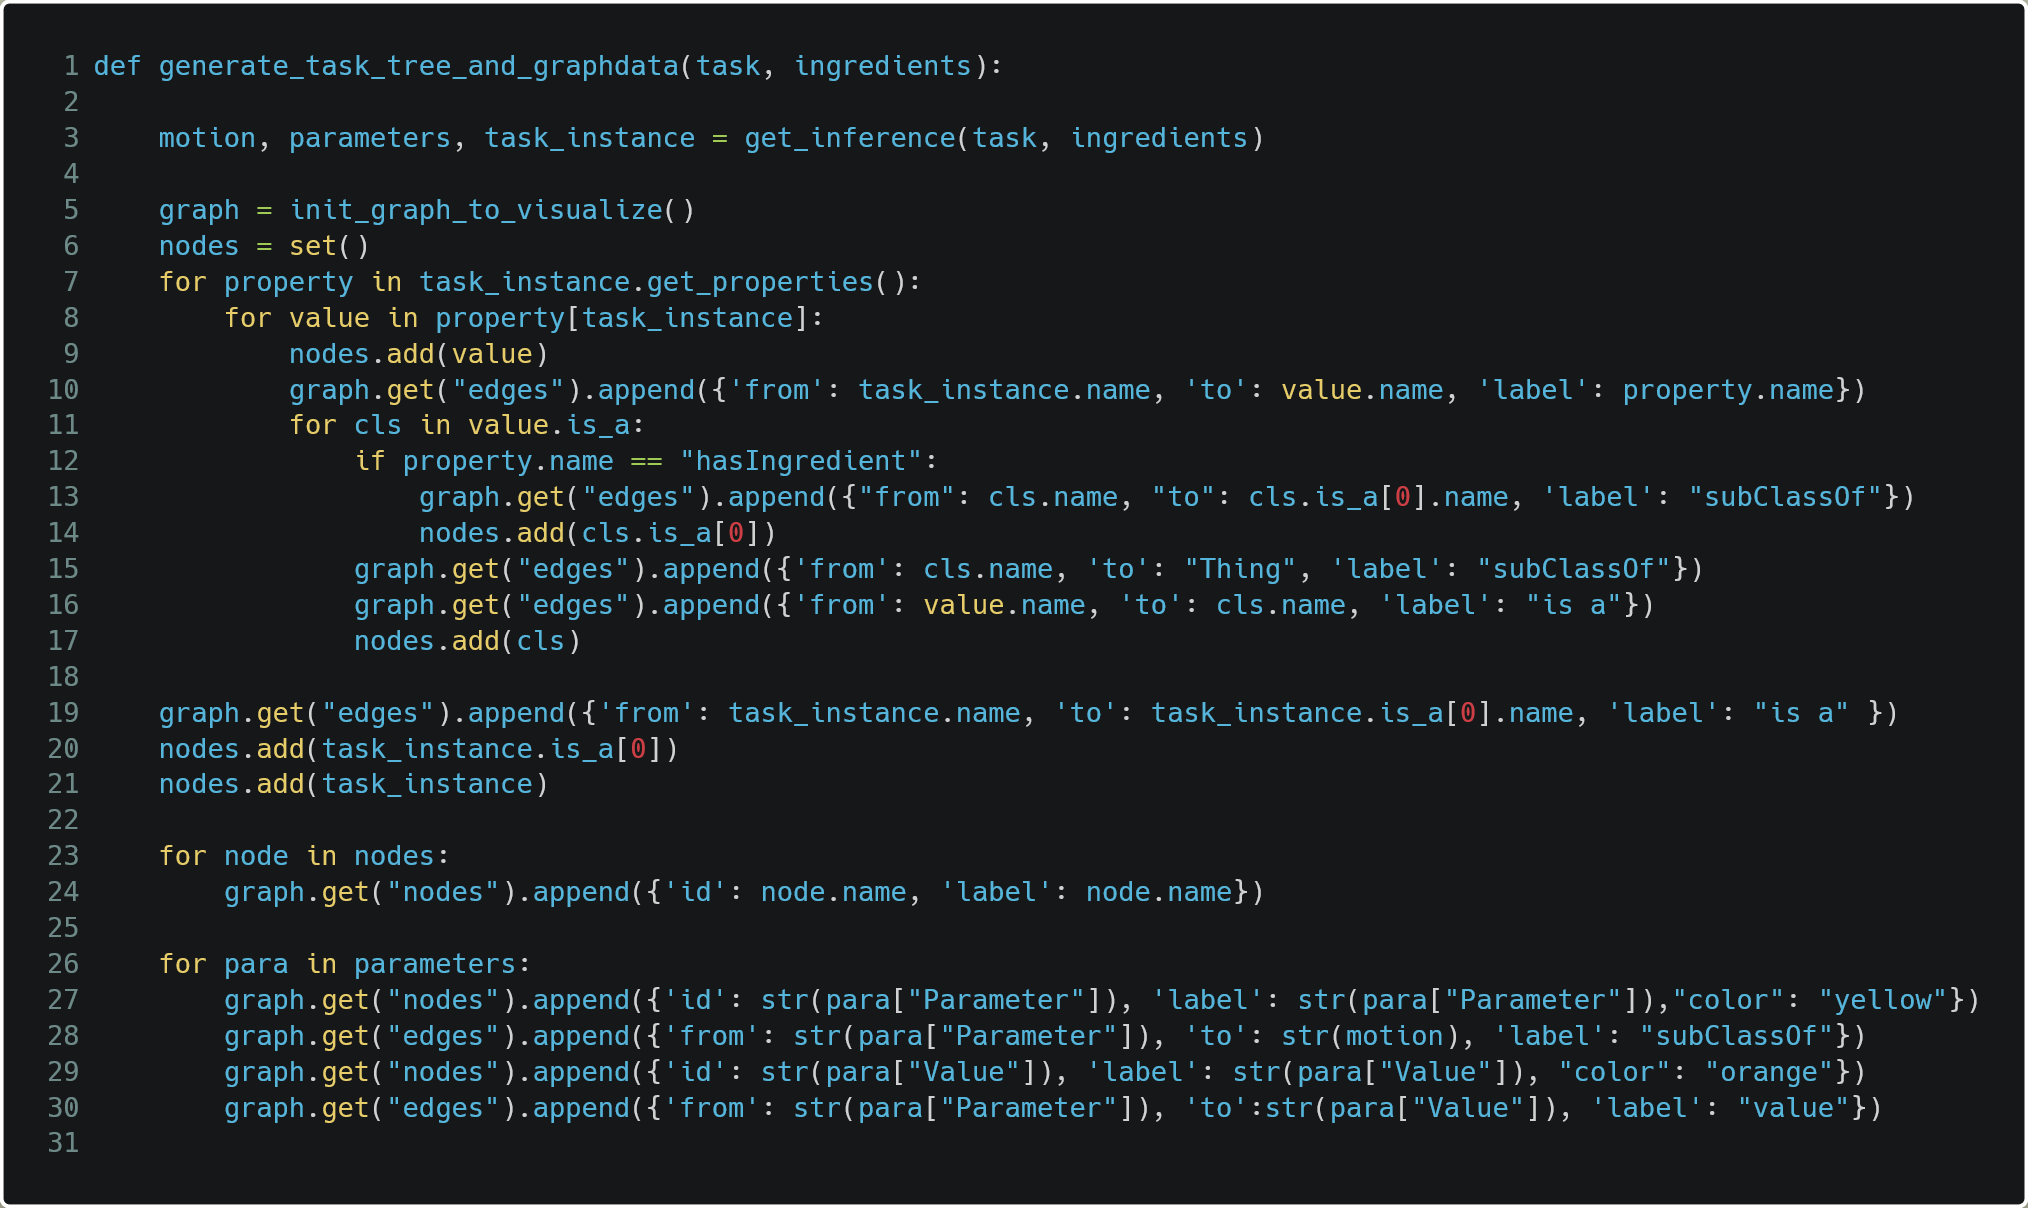
\includegraphics[scale=0.2]{Graphics/get_graph_data_new.png}
    \caption{generating the visualized graph and task tree}
\end{figure}

\begin{itemize}
    \item Line 3: The results of the inference function (see: \nameref{par:Inference}) are stored and used for further processing.
    \item Lines 5 and 6: We initialize an empty graph, which will be filled with nodes and edges throughout the function. Additionally, a set is initialized for the set of nodes.
    \item Lines 7 to 17: Based on the task instance, the graph is structured starting from this node. It checks which relations exist for this instance and accordingly inserts into the set of edges and nodes. Additionally, for the \textit{hasIngredient} relation, the superclass of the ingredient is considered. Finally, the edge labeling is chosen based on the relation, and the classes are added to the graph.
    \item Lines 19 to 21: The task instance itself is processed and added to the graph.
    \item Lines 23 and 24: Iterating over the set of nodes, they are added to the graph.
    \item Lines 26 to 30: The inferred parameters are processed and added to the graph in the end.
\end{itemize}

For the task tree, we create a 3-column table. The first column represents the step, the second column represents the action, and the third column represents the parameters used to illustrate them. The task tree is a list of entries, which can also contain dynamic data such as motions and ingredients.
\begin{figure}[H]
    \includegraphics[scale=0.2]{Graphics/get_graph_data_new2ä.png}
    \caption{generating the visualized graph and task tree}
\end{figure}

\begin{itemize}
    \item 1: The first entry pertains to the robot's action, which is to choose a tool for the upcoming actions. The list of \textit{Tools} corresponds to the subclasses of \textit{Tools} from the ontology. (REFERENCE TO GET TOOLS LEAF)
    \item 2 and 3: Analogous to the first entry, the container is chosen and must be held with an arm for the upcoming motion.
    \item 4: This action describes the starting point of the motion; each motion has its own starting point (see: \nameref{chap:Motions}).
    \item 5: In this step, it is explained with which parameters the motion must be executed.
    \item 6: Once the motion execution is complete, the used tool is set aside.
    \item 7: The final step does nothing but announce the end of the task tree.
    \end{itemize}

These data are forwarded to the frontend via the \textit{flask} interface, where ultimately the graph and the task tree are visualized (see: \ref{fig:graph_inferred})

\subsection(Weaknesses)
\paragraph{Using vis.js}
Using the graph visualization library vis.js yields poor performance on large graphs.
This reason is known to the developers of vis.js (See reference) and the cause of the problem is coming
from the physics simulation. The visualized graph is a force directed graph and the physics simulation attempts to make a user readable graph 
by seperating and clustering nodes who don't or belong to each other. This is done iteratively and consumes a lot of time for large sets of nodes
connected via many edges. The more interconnected the graph is the more terrible the performance gets. 

\paragraph{Data Visualizer}
This framework in its core is not a graph data visualizer. While it is absolutely able to display relationships and attributes of instance data, visualizing 
large datasets defined as ontology is not feasible. It is limited by vis.js which is poorly optimised for large sets of nodes and edges. 
Thus this framework can't be a graph data visualizer. 

\section{Fazit -}

\chapter{Conclusion}
\label{chap:conclusion}

\section{Summary}
This master thesis is a proof of concept in which we explained in detail how a robotic system like the PR2 
using the robotic cognitive architecture \textit{CRAM} is able to mix in simulation. 

Implementing various motions in \textit{Cram} could only be done through.

The underlying model - a knowledgebase models several relevant aspects of a mixing action. 
Ingredients which are being mixed, the types of motion which can be executed, the type of container to 
store the ingredients and to mix in and the tools to perform the mixing actions. By keeping the model simple we achieve that the robot 
is able to infer motions through the rules based language SWRL. 

Our modelled motions don't implement how a motion is executed but rather it gives capabilities via parameters to adapt 
to various containers and tools. The implemenation of each motion - \textbf{Circular}, \textbf{Folding}, \textbf{Horizontal Elliptical} 
and \textbf{Whirlstom}, is available in pycram, any robotic system able to employ \textit{Cram}, can execute these motions. 

Additionally to this proof a concept we implemented a different way of visualizing ontologies, by focusing 
on complex class expressions which haven't been done before. Using the \textit{OWLVisualizer} a user is able to query 
complex class expressions without knowing how to write \textit{SPARQL} queries. The \textit{OWLVisualizer} will generate A
\textit{SPARQL} query for the user applying triple matching to get the queried graph. This query can be adjusted 
to the needs of the user, by changing the contents of the query without changing the triple matching. 


- Data aqcuired and Structured.
- Modelled a queryable Knowledgebase
- Adapted motions
- Proof Of Concept
- Graphviz
\section{Future Work}
This proof of concept was established in \textit{Cram} in simulation. In simulations many things are simple.
The robot has ground truth for each available object, the ingredients to mix, the tools to perform mixing, the container to mix in. 
To move ahead, our proof of concept should be implemented on a real robot, to see how much more difficult it will 
be in real world scenarios.

With regards to future work many limitations arose during implementation of our proof of concept.
Our motions are effectively 2D motions, where one axis is not changing over the course of the motion.
Moving from simulation to real world, it will be necessary to include dives into each motion, so that 
the substances are properly mixed. 

Another limiting aspect is the lack of collision detection. As of now, we ensure that the tool is not colliding 
with objects only with respect to 2 out of 3 axes. If the tool is placed to low, and the container has a spherical shape and not 
cuboid shape, the tool will eventually collide with the object. To tackle this limitation, we require depth-based perception
and various techniques to find out optimal height for the tool during execution of a mixing action.

Once we move to real world we loose ground truth on all relevant objects required for mixing.
Here we will need perception frameworks capable of detecting and locating objects in a scene, 
picking and placing objects and different kinds of actions for example pouring, to fill a container
with ingredients.

In simulation the robot will not fail unless the inference fails. As long as a motion is inferred, mixing will be executed.
This has to be adjusted



- Diving motions
- Prediction substances
- Deployment on real robot
- Uncertainity. -> Object Detection
- Failure Handling

\section{Last Words}

- GEOMETRIE IN EINLEITUNG BETRACHTEN.
keine fragen in EINLEITUNG
\bibliography{literature}

\chapter{Appendix}
\label{chap:appendix}

\section{Video Analysis}
\section{Evaluation}
Im Anhang möchten wir an der im \nameref{sec:evaluation} vorgestellten Konzept anknüpfen.
Hier werden wir die Tabellen detaillierter darstellen und möglichst viele Szenarios abdecken.
Nochmal zur Erinnerung: Eine Kombination von einer Task und einer Menge von Ingredients inferriert Motions, welche wiederrum mit Parameter verbunden sind.
Diese Parameter dienen zur Motionanpassung abhänging vom gewählten Tool und Container. 
Letzendlich muss berechnet werden in welchem Bereich die Motion ausgeführt werden kann.
Die Berechnung lautet wie folgt:
\begin{lstlisting}
    radius_upper_bound = ((dim[0] * radius_bounds[0]) - 
        max(dim2[0], dim2[1])) / 2

    radius_lower_bound = max(0, ((dim[0] * radius_bounds[1]) - 
        max(dim2[0], dim2[1])) / 2)
\end{lstlisting}
wobei die Dimensionsparameter wie folgt definiert werden: 
\begin{lstlisting}
    dim = [max(obj_dim[0], obj_dim[1]), 
        min(obj_dim[0], obj_dim[1]), obj_dim[2]]

    dim2 = [max(tool_dim[0], tool_dim[1]), 
        min(tool_dim[0], tool_dim[1]), tool_dim[2]]
\end{lstlisting}

\textit{tool\_dim} und \textit{obj\_dim} entsprechen jeweils der Dimension des Tools und des Containers.
Mit dieser Berechnung ist es dann möglich einen Aktionsradius zu definieren, um die Motion gefahrlos auszuführen, also ohne dass der Tool zum Beispiel gegen die Kante des Containers schlagen würde.

Im Folgenden möchten wir beweisen, dass unser System sich der Umgebung anpasst und die Aktionsradien abhänging von den gegebenen Dimensionen berechnet.

Anmerkungen: 
\begin{itemize}
    \item Die Radius Bounds ist eine Liste von zwei Elementen wobei das erste Element, dem Radius der oberen Schranke entspricht und das zweite Element dem Radius der unteren Schranke.
    \item Manche Kombinationen von Task und Ingredient ergeben die selbe Motion und werden in diesem Fall zusammengefasst. 
    \item Es kann vorkommen, dass der Aktionsradius negativ ist, hierbei ist Finetuning notwending, allgemein sollte bei negativem Aktionsradius die Bewegung nicht ausgeführt werden. Allerdings könnte man für relativ kleine Radien, eine Ausnahmen einfügen.
    \item Die Tools Spoon und Fork werden nicht getrennt betrachtet, da diese in der relevanten Form und Größe sich sehr ähneln.
    \item Folding Task inferriert die selben Parameter unabhängig der Zutaten.
    \item \textbf{Whisk Dimensions:} \textit{0.11, 0.08, 0.31}
    \item \textbf{Wooden Spoon Dimensions:} \textit{0.09, 0.095, 0.29}
    \item \textbf{Fork Dimensions:} \textit{0.06, 0.04, 0.25}
    \item \textbf{Salad Bowl Dimensions:} \textit{0.25, 0.25, 0.11}
    \item \textbf{Pot Dimensions:} \textit{0.31, 0.37, 0.11}
    \item \textbf{Small Bowl Dimensions:} \textit{0.14, 0.14, 0.07}
\end{itemize}

\subsection{Mixing Task}
\subsubsection{Liquid, Powder, Liquid and Powder, Liquid and Semi-Liquid}
\begin{itemize}
    \item \textbf{Inferred Motions:} \textit{Whirlstorm Motion}
    \item \textbf{Inferred Parmaters:} \textit{0.7, 0.0}
\end{itemize}

\begin{table}[H]
    \centering
    \begin{tabular}{|c|c|c|c|c|}
      \hline
      \textbf{Tool} & \textbf{Container} & \textbf{Action Radius}\\
      \hline
      Whisk & Salad Bowl & [0.033, 0] \\
      \hline
      Whisk & Pot & [0.075, 0] \\
      \hline
      Whisk & Small Bowl & [-0.004, 0]\\
      \hline
      Wooden Spoon & Salad Bowl & [0.04, 0] \\
      \hline
      Wooden Spoon & Pot & [0.082, 0] \\
      \hline
      Wooden Spoon & Small Bowl & [0.003, 0] \\
      \hline
      Fork & Salad Bowl & [0.058, 0] \\
      \hline
      Fork & Pot & [0.1, 0] \\
      \hline
      Fork & Small Bowl & [0.03, 0] \\
      \hline
    \end{tabular}
    \caption{Mixing Task which infer Whirlstorm Motion}
    
  \end{table}



\subsubsection{Semi-Liquid, Powder and Semi-Liquid}
\begin{itemize}
    \item \textbf{Inferred Motions:} \textit{Whirlstorm Motion, Horizontal Eliptical Motion}
    \item \textbf{Inferred Parmaters:} \textit{0.7, 0.0} and \textit{ellipse shift: 0.04}
\end{itemize}
  
\begin{table}[H]
    \centering
    \begin{tabular}{|c|c|c|c|c|}
    \hline
    \textbf{Tool} & \textbf{Container} & \textbf{Action Radius}\\
    \hline
    Whisk & Salad Bowl & [0.033, 0] \\
    \hline
    Whisk & Pot & [0.075, 0] \\
    \hline
    Whisk & Small Bowl & [-0.004, 0]\\
    \hline
    Wooden Spoon & Salad Bowl & [0.04, 0] \\
    \hline
    Wooden Spoon & Pot & [0.082, 0] \\
    \hline
    Wooden Spoon & Small Bowl & [0.003, 0] \\
    \hline
    Fork & Salad Bowl & [0.058, 0] \\
    \hline
    Fork & Pot & [0.1, 0] \\
    \hline
    Fork & Small Bowl & [0.03, 0] \\
    \hline
\end{tabular}
\caption{Mixing Task that infer Whirlstorm and Horizontal Eliptical Motion}

\end{table}

\subsection{Stirring Task}

\subsubsection{Liquid, Liquid and Powder}

\begin{itemize}
    \item \textbf{Inferred Motion:} \textit{Circular Motion}
    \item \textbf{Inferred Parameters:} \textit{0.7, 0.7}
\end{itemize}
\begin{table}[H]
    \centering
    \begin{tabular}{|c|c|c|c|c|}
      \hline
      \textbf{Tool} & \textbf{Container} & \textbf{Action Radius}\\
      \hline
      Whisk & Salad Bowl & [0.033, 0.033] \\
      \hline
      Whisk & Pot & [0.075, 0.075] \\
      \hline
      Whisk & Small Bowl & [-0.004, -0.004]\\
      \hline
      Wooden Spoon & Salad Bowl & [0.04, 0.04] \\
      \hline
      Wooden Spoon & Pot & [0.082, 0.082] \\
      \hline
      Wooden Spoon & Small Bowl & [0.003, 0.003] \\
      \hline
      Fork & Salad Bowl & [0.058, 0.058] \\
      \hline
      Fork & Pot & [0.1, 0.1] \\
      \hline
      Fork & Small Bowl & [0.03, 0.03] \\
      \hline
    \end{tabular}
    \caption{Stirring Task which infer Circular Motion}
    
  \end{table}

\subsubsection*{Powder}
\begin{itemize}
    \item \textbf{Inferred Motions:} \textit{Whirlstorm Motion}
    \item \textbf{Inferred Parmaters:} \textit{0.7, 0.0}
\end{itemize}
\begin{table}[H]
    \centering
    \begin{tabular}{|c|c|c|c|c|}
      \hline
      \textbf{Tool} & \textbf{Container} & \textbf{Action Radius}\\
      \hline
      Whisk & Salad Bowl & [0.033, 0] \\
      \hline
      Whisk & Pot & [0.075, 0] \\
      \hline
      Whisk & Small Bowl & [-0.004, 0]\\
      \hline
      Wooden Spoon & Salad Bowl & [0.04, 0] \\
      \hline
      Wooden Spoon & Pot & [0.082, 0] \\
      \hline
      Wooden Spoon & Small Bowl & [0.003, 0] \\
      \hline
      Fork & Salad Bowl & [0.058, 0] \\
      \hline
      Fork & Pot & [0.1, 0] \\
      \hline
      Fork & Small Bowl & [0.03, 0] \\
      \hline
    \end{tabular}
    \caption{Stirring Task which infer Whirlstorm Motion}
    
  \end{table}

\subsubsection{Semi-Liquid, Semi-Liquid and Liquid, Semi-Liquid and Powder}
\begin{itemize}
    \item \textbf{Inferred Motions:} \textit{Whirlstorm Motion, Horizontal Eliptical Motion}
    \item \textbf{Inferred Parmaters:} \textit{0.7, 0.0} and \textit{ellipse shift: 0.04}
\end{itemize}
  
\begin{table}[H]
    \centering
    \begin{tabular}{|c|c|c|c|c|}
    \hline
    \textbf{Tool} & \textbf{Container} & \textbf{Action Radius}\\
    \hline
    Whisk & Salad Bowl & [0.033, 0] \\
    \hline
    Whisk & Pot & [0.075, 0] \\
    \hline
    Whisk & Small Bowl & [-0.004, 0]\\
    \hline
    Wooden Spoon & Salad Bowl & [0.04, 0] \\
    \hline
    Wooden Spoon & Pot & [0.082, 0] \\
    \hline
    Wooden Spoon & Small Bowl & [0.003, 0] \\
    \hline
    Fork & Salad Bowl & [0.058, 0] \\
    \hline
    Fork & Pot & [0.1, 0] \\
    \hline
    Fork & Small Bowl & [0.03, 0] \\
    \hline
\end{tabular}
\caption{Stirring Task that infer Whirlstorm and Horizontal Eliptical Motion}

\end{table}

\subsection{Beating Task}
\subsubsection{Liquid, Liquid and Powder}
\begin{itemize}
    \item \textbf{Inferred Motions:} \textit{Whirlstorm Motion}
    \item \textbf{Inferred Parmaters:} \textit{0.7, 0.0}
\end{itemize}
\begin{table}[H]
    \centering
    \begin{tabular}{|c|c|c|c|c|}
      \hline
      \textbf{Tool} & \textbf{Container} & \textbf{Action Radius}\\
      \hline
      Whisk & Salad Bowl & [0.033, 0] \\
      \hline
      Whisk & Pot & [0.075, 0] \\
      \hline
      Whisk & Small Bowl & [-0.004, 0]\\
      \hline
      Wooden Spoon & Salad Bowl & [0.04, 0] \\
      \hline
      Wooden Spoon & Pot & [0.082, 0] \\
      \hline
      Wooden Spoon & Small Bowl & [0.003, 0] \\
      \hline
      Fork & Salad Bowl & [0.058, 0] \\
      \hline
      Fork & Pot & [0.1, 0] \\
      \hline
      Fork & Small Bowl & [0.03, 0] \\
      \hline
    \end{tabular}
    \caption{Beating Task which infer Whirlstorm Motion}
    
  \end{table}

\subsubsection*{Powder, Semi-Liquid, Liquid and Semi-Liquid}
\begin{itemize}
    \item \textbf{Inferred Motions:} \textit{Whirlstorm Motion, Horizontal Eliptical Motion}
    \item \textbf{Inferred Parmaters:} \textit{0.7, 0.0} and \textit{ellipse shift: 0.04}
\end{itemize}
  
\begin{table}[H]
    \centering
    \begin{tabular}{|c|c|c|c|c|}
    \hline
    \textbf{Tool} & \textbf{Container} & \textbf{Action Radius}\\
    \hline
    Whisk & Salad Bowl & [0.033, 0] \\
    \hline
    Whisk & Pot & [0.075, 0] \\
    \hline
    Whisk & Small Bowl & [-0.004, 0]\\
    \hline
    Wooden Spoon & Salad Bowl & [0.04, 0] \\
    \hline
    Wooden Spoon & Pot & [0.082, 0] \\
    \hline
    Wooden Spoon & Small Bowl & [0.003, 0] \\
    \hline
    Fork & Salad Bowl & [0.058, 0] \\
    \hline
    Fork & Pot & [0.1, 0] \\
    \hline
    Fork & Small Bowl & [0.03, 0] \\
    \hline
\end{tabular}
\caption{Beating Task which infer Whirlstorm and Horizontal Eliptical Motion}

\end{table}

\subsubsection*{Powder and Semi-Liquid}
\begin{itemize}
    \item \textbf{Inferred Motions:} \textit{Horizontal Eliptical Motion}
    \item \textbf{Inferred Parmaters:} \textit{0.7, 0.0} and \textit{ellipse shift: 0.04}
\end{itemize}
  
\begin{table}[H]
    \centering
    \begin{tabular}{|c|c|c|c|c|}
    \hline
    \textbf{Tool} & \textbf{Container} & \textbf{Action Radius}\\
    \hline
    Whisk & Salad Bowl & [0.033, 0] \\
    \hline
    Whisk & Pot & [0.075, 0] \\
    \hline
    Whisk & Small Bowl & [-0.004, 0]\\
    \hline
    Wooden Spoon & Salad Bowl & [0.04, 0] \\
    \hline
    Wooden Spoon & Pot & [0.082, 0] \\
    \hline
    Wooden Spoon & Small Bowl & [0.003, 0] \\
    \hline
    Fork & Salad Bowl & [0.058, 0] \\
    \hline
    Fork & Pot & [0.1, 0] \\
    \hline
    Fork & Small Bowl & [0.03, 0] \\
    \hline
\end{tabular}
\caption{Beating Task which infer Horizontal Eliptical Motion}

\end{table}


\subsection{Whisking Task}
\subsubsection{Liquid, Powder, Liquid and Powder, Liquid and Semi-Liquid, Semi-Liquid and Powder}
\begin{itemize}
    \item \textbf{Inferred Motions:} \textit{Whirlstorm Motion}
    \item \textbf{Inferred Parmaters:} \textit{0.7, 0.0}
\end{itemize}
\begin{table}[H]
    \centering
    \begin{tabular}{|c|c|c|c|c|}
      \hline
      \textbf{Tool} & \textbf{Container} & \textbf{Action Radius}\\
      \hline
      Whisk & Salad Bowl & [0.033, 0] \\
      \hline
      Whisk & Pot & [0.075, 0] \\
      \hline
      Whisk & Small Bowl & [-0.004, 0]\\
      \hline
      Wooden Spoon & Salad Bowl & [0.04, 0] \\
      \hline
      Wooden Spoon & Pot & [0.082, 0] \\
      \hline
      Wooden Spoon & Small Bowl & [0.003, 0] \\
      \hline
      Fork & Salad Bowl & [0.058, 0] \\
      \hline
      Fork & Pot & [0.1, 0] \\
      \hline
      Fork & Small Bowl & [0.03, 0] \\
      \hline
    \end{tabular}
    \caption{Whisking Task which infer Whirlstorm Motion}
    
  \end{table}

  \subsubsection*{Semi-Liquid}
  \begin{itemize}
      \item \textbf{Inferred Motions:} \textit{Horizontal Eliptical Motion}
      \item \textbf{Inferred Parmaters:} \textit{0.7, 0.0} and \textit{ellipse shift: 0.04}
  \end{itemize}
    
  \begin{table}[H]
      \centering
      \begin{tabular}{|c|c|c|c|c|}
      \hline
      \textbf{Tool} & \textbf{Container} & \textbf{Action Radius}\\
      \hline
      Whisk & Salad Bowl & [0.033, 0] \\
      \hline
      Whisk & Pot & [0.075, 0] \\
      \hline
      Whisk & Small Bowl & [-0.004, 0]\\
      \hline
      Wooden Spoon & Salad Bowl & [0.04, 0] \\
      \hline
      Wooden Spoon & Pot & [0.082, 0] \\
      \hline
      Wooden Spoon & Small Bowl & [0.003, 0] \\
      \hline
      Fork & Salad Bowl & [0.058, 0] \\
      \hline
      Fork & Pot & [0.1, 0] \\
      \hline
      Fork & Small Bowl & [0.03, 0] \\
      \hline
  \end{tabular}
  \caption{Whisking Task which infer Horizontal Eliptical Motion}
  
  \end{table}

\subsection{Folding Task}
\subsubsection{Every Ingredient}

\begin{itemize}
    \item \textbf{Inferred Motions:} \textit{Folding Motion}
    \item \textbf{Inferred Parmaters:} \textit{0.7, 0.0}; \textit{repetitive folding rotation shift: 22.5} and \textit{folding rotation shift: 90}
\end{itemize}
  
\begin{table}[H]
    \centering
    \begin{tabular}{|c|c|c|c|c|}
    \hline
    \textbf{Tool} & \textbf{Container} & \textbf{Action Radius}\\
    \hline
    Whisk & Salad Bowl & [0.033, 0] \\
    \hline
    Whisk & Pot & [0.075, 0] \\
    \hline
    Whisk & Small Bowl & [-0.004, 0]\\
    \hline
    Wooden Spoon & Salad Bowl & [0.04, 0] \\
    \hline
    Wooden Spoon & Pot & [0.082, 0] \\
    \hline
    Wooden Spoon & Small Bowl & [0.003, 0] \\
    \hline
    Fork & Salad Bowl & [0.058, 0] \\
    \hline
    Fork & Pot & [0.1, 0] \\
    \hline
    Fork & Small Bowl & [0.03, 0] \\
    \hline
\end{tabular}
\caption{Folding Task}

\end{table}
\end{document}

